\documentclass[fleqn,reqno,10pt,draft]{article}


\usepackage[natbib=true,
            style=authoryear-comp,
            backend=bibtex,
            sortcites=false,
            maxnames=2,
            doi=false,
            url=false]{biblatex}
\bibliography{MyRefGlobal}
% \bibliography{paper}

\usepackage[final,            % override "draft" which means "no nothing"
            colorlinks,       % rather than outlining them in boxes
            linkcolor=gray,   % override truly awful color choices
            citecolor=gray,   %   (ditto)
            urlcolor=gray,    %   (ditto)
            plainpages=false, % to overcome complaints with multiple
            pdfpagelabels,    % multiple page 1-s due to preface
            hypertexnames=false % solves warning, but interferes with
                                % index and \autoref apparently
            ]{hyperref}


\usepackage{amsmath}            % Formeln
\usepackage{amsfonts}           % Fonts for Formulas
\usepackage{amssymb}
\usepackage[final]{graphicx}
\usepackage{booktabs}
\usepackage{enumerate}
\usepackage{lipsum}
\usepackage{txfonts} % for strict implication symbols
\usepackage{soul}
\usepackage{relsize} % provides command \relsize{+/-x} for relative
                     % font size changes
\usepackage[german,english]{babel}
\usepackage[utf8]{inputenc}
\usepackage[T1]{fontenc} 
\usepackage{subfig}
\usepackage{xypic}
\usepackage{url}
\usepackage{tikz}
\usetikzlibrary{arrows,shapes,automata,backgrounds,petri,fit,decorations.pathmorphing}
\usepackage{refcount}
\usepackage{xspace} % for \xspace in definition of acronyms etc.
\usepackage{attrib} % for right-aligned references at the end of
                    % quotes; part of Frankenstein bundle, but 
\renewcommand\PreTrib {}   % overwrite these commands, from attrib.sty
\renewcommand\PostTrib {}  % to suppress additional brackets around
                           % attributions
\usepackage{eurosym}
\usepackage{pgfplots}
\usepackage{todonotes}

\usepackage{../helpers/gb4e_micha}
\usepackage{../helpers/proofing}

\usepackage{../helpers/mycommands}
% \usepackage{../helpers/myenvironments}


% \usepackage{geometry}
% \linespread{1.2}

%%%% Additional Macros

\newcommand{\lit}{\acro{lit}}
\newcommand{\glb}{\acro{glb}}
\newcommand{\loc}{\acro{loc}}

\newcommand{\as}{\acro{as}}
\renewcommand{\es}{\acro{es}}
\renewcommand{\AE}{\as}
\newcommand{\GE}{\es}
\newcommand{\ea}{\acro{ea}}

\newcommand{\lc}{\acro{lc}}
\newcommand{\ec}{\acro{ec}}
\newcommand{\LC}{\lc}
\newcommand{\EC}{\ec}

\newcommand{\exh}{\ensuremath{\mathrm{Exh}}}
\newcommand{\alt}{\ensuremath{\mathrm{Alt}}}

\newcommand{\ivt}{\acro{ivt}}

\renewcommand{\mymark}[1]{\textbf{#1}}

\pgfplotscreateplotcyclelist{mylist}{% 
    {solid,black},
    {dotted,black}, 
    {dashed,black}, 
    {loosely dotted,gray}, 
    {solid,black},
    {dotted,black},
    {dashed,black},
    {loosely dotted}}

\usetikzlibrary{calc}
\usepackage{nicefrac}

%%%% Document

\title{Embedded Scalars: {A}n Experimental Revisit} \author{Fabian
  Schlotterbeck, Michael Franke and Petra Augurzky} \date{}

\begin{document}
\maketitle



\begin{abstract}
  Scalar item \emph{some} is widely assumed to receive a pragmatic
  meaning enrichment to \emph{some but not all} if it occurs in matrix
  position. The question under which circumstances this enrichment can
  occur in certain embedded positions plays an important role in
  deciding how to delineate semantics and pragmatics. % Some claim
  % that it requires marked intonation for the relevant pragmatic
  % enrichment to occur in embedded position; others allow for it more
  % freely.
  We present new experimental data that bears on this theoretical
  issue. In distinction to previous experimental approaches, we
  presented sentence material auditorily in order to explicitly
  control prosodic markedness of the scalar item. Moreover, our
  experimental design gives insight into the preference of
  hypothesized meaning differences, not only on their general
  availability. The data obtained in this way turns out problematic
  for both a traditional Gricean view of scalar implicature
  calculation, as well as the more recent grammatical approach.
\end{abstract}




\section{Introduction}
\label{sec:introduction}

The existential quantifier \emph{some} is usually assumed to receive a
semantic interpretation similar to logical $\exists$, so that
(\ref{bsp:Plain-SI-Target}) is literally true even when Hans solved
all of the problems. But it is also usually considered to invite
comparison with (at least) the semantically stronger universal
quantifier \emph{all}
\citep[c.f.][]{Horn1972:On-the-Semantic,Gazdar1979:Pragmatics:-Imp,AtlasLevinson1981}. This
scalar comparison can lead to an upper-bound meaning enrichment, e.g.,
when an utterance of (\ref{bsp:Plain-SI-Target}) is taken to invite
the inference in (\ref{bsp:Plain-SI-Implicature}).

\begin{exe}
  \ex \label{bsp:Plain-SI}
    \begin{xlist}
      \ex \label{bsp:Plain-SI-Target} Hans solved some of the
        problems.
      \ex \label{bsp:Plain-SI-Implicature} $\implicates$ Hans solved
        some but not all of the problems.
      \ex \label{bsp:Plain-SI-Alternative} Hans solved all of the problems.
    \end{xlist}
\end{exe}

\noindent The classical explanation of this inference, following the
pioneering work of \citet{Grice1975:Logic-and-Conve}, is that
(\ref{bsp:Plain-SI-Implicature}) is a pragmatic inference, a so-called
\emph{quantity implicature}, derived by an abductive inference as the
best explanation of why informed, knowledgable and cooperative
speakers would utter (\ref{bsp:Plain-SI-Target}) when they could also
utter the semantically stronger and relevant
(\ref{bsp:Plain-SI-Alternative}) \citep[see][for
recent overview]{Geurts2010:Quantity-Implic}.


% If this upper-bound inference would occur often and
% systematically enough, then it may well be that also embedded
% occurrences of \emph{some} get enriched, in some fashion or other, to
% contribute the enriched meaning \emph{some but not all} also under the
% scope of other logical operators.
% Indeed, even
% \citeauthor{Grice1975:Logic-and-Conve} envisaged this possibility when
% he wrote: ``It may not be impossible for what starts life, so to
% speak, as a conversational implicature to become conventionalized''
% \citep[p.58]{Grice1975:Logic-and-Conve}.


This paper deals with the interpretation of two types of sentences,
where the scalar item \emph{some} occurs in the scope of other logical
operators. In \as-sentences (mnemonic for \textit{all \dots some
  \dots}) as in (\ref{bsp:AE}) the scalar item \emph{some} is embedded
under universal quantifier \emph{all}. In \es-sentences (mnemonic for
\textit{exactly one \dots some \dots}) like (\ref{bsp:GE}) \emph{some}
takes scope under the non-monotonic quantifier \emph{exactly one}.
According to current pragmatic theory, there are at least three
relevant candidate readings for \as- and \es-sentences: (i) a
\emph{literal reading} like in (\ref{bsp:AE-Literal}) and
(\ref{bsp:GE-Literal}) where \emph{some} has only its literal meaning;
(ii) a \emph{global reading} like in (\ref{bsp:AE-Global}) and
(\ref{bsp:GE-Global}) where we enrich the meaning of (\ref{bsp:AE})
and (\ref{bsp:GE}) with the negation of the corresponding sentences
(\ref{bsp:AE-Alternative}) and (\ref{bsp:GE-Alternative}) where
\emph{some} is replaced by \emph{all}; and also (iii) a \emph{local
  reading} like in (\ref{bsp:AE-Local}) and (\ref{bsp:GE-Local}) where
\emph{some} is interpreted as \emph{some but not all} in the scope of
the embedding quantifier.


\begin{exe}
  \ex \label{bsp:AE} \mymark{All} of the students read {\mymark{some}} of the
  papers. \hfill{(\as)}

  \begin{xlist}
  \ex \label{bsp:AE-Literal} \mymark{All} of the students read
    {\mymark{some and maybe all}} of the papers. \hfill (\as-\lit)
  \ex \label{bsp:AE-Global}
    \mymark{All} of the students read \mymark{some and maybe all} 
    and  \hfill (\as-\glb)\\
    it's not the case that \mymark{all} of the students read \mymark{all} of the papers.
  \ex \label{bsp:AE-Local}
    \mymark{All} of the students read {\mymark{some  but not all}} of the
    papers. \hfill (\as-\loc)
  \end{xlist}
\end{exe}

\begin{exe}
\ex  \label{bsp:GE} \mymark{Exactly one} of the students read {\mymark{some}} of the
  papers. \hfill{(\es)}

  \begin{xlist}
  \ex \label{bsp:GE-Literal} \mymark{Exactly one} of the students read
    {\mymark{some and maybe all}} of the papers. \hfill (\es-\lit)
  \ex \label{bsp:GE-Global}
    \mymark{Exactly one} of the students read \mymark{some and maybe all} 
    and  \hfill (\es-\glb)\\
    it's not the case that \mymark{exactly one} of the students read \mymark{all} of the papers.
  \ex \label{bsp:GE-Local}
    \mymark{Exactly one} of the students read {\mymark{some  but not all}} of the
    papers. \hfill (\es-\loc)
  \end{xlist}
\end{exe}


\begin{exe}
\ex \label{bsp:AE-Alternative} \mymark{All} of the students read
  {\mymark{all}} of the papers. 

\ex \label{bsp:GE-Alternative} \mymark{Exactly one} of the students
  read {\mymark{all}} of the papers.
\end{exe}

% Section~\ref{sec:get-know-your} will discuss these readings
% in more detail, showing that all three readings of each sentence are
% distinct but logically dependent on each other in interesting ways.

\noindent Given this plurality of hypothesized readings, we need to
ask:
\begin{enumerate}[Q1:]
\item which of these readings are available to na\"{i}ve subjects; and
\item which of the available readings are preferred.\fn{It may
    ultimately be impossible to keep unavailability and strong
    dispreference strictly apart. For our purposes this is not
    important. Every time we speak of availability, the so-inclined
    reader may think of non-negligible preference.}
\end{enumerate}
Addressing these questions empirically is relevant because they lie at
the heart of the current debate about the exact location and nature of
the interface between semantics and pragmatics. The controversy
concerns the question under which circumstances and to what extent the
upper-bound inference from \emph{some} to \emph{some but not all} can
occur within the compositional computation of semantic values. Two
opposing theoretical positions can be distinguished here:
\emph{traditionalism} holds in particular that local readings should
not be readily attested unless marked by special intonation;
\emph{grammaticalism} holds that local readings are available and, at
least under the most prominent of selection principles for candidate
readings, even preferred (see Section~\ref{sec:grammaticalism}). To
distinguish between these opposing positions, it is therefore
necessary to assess the availability and relative preference of
readings for \as- and \es-sentences under conditions that control for
intonational markedness. This is what this paper aims to do.


A number of empirical studies have already studied sentences like
(\ref{bsp:AE}) and (\ref{bsp:GE}) this issue
\citep[e.g.][]{GeurtsPouscoulous2009:Embedded-Implic,CliftonDube2010:Embedded-Implic,ChemlaSpector2010:Experimental-Ev}. Unfortunately,
results from these studies do not provide uncontroversial evidence to
decide between the two main rivaling positions. This is due to several
reasons. Firstly, previous studies have only accumulated limited
evidence pertaining to the preference relations between putative
readings of both types of sentences. Secondly, as
\citet{Tielvan-Tiel2012:Embedded-Scalar} and
\citet{GeurtsTielvan-Tiel2013:Scalar-expressi} argue, the putative
evidence for the availability of local readings of \as-sentences
suggested by studies of \citet{CliftonDube2010:Embedded-Implic} and
\citet{ChemlaSpector2010:Experimental-Ev}, might well be confounds
with what van Tiel and Geurts call \emph{typicality effects}. Finally,
and most importantly, previous studies presented target sentences
visually. This is highly problematic, because traditionalists admit to
the availability of local readings as long as it is intonationally
marked
\citep[e.g.][]{Horn2006:The-Border-Wars,Geurts2009:Scalar-Implicat,ChemlaSpector2010:Experimental-Ev,Geurts2010:Quantity-Implic,Tielvan-Tiel2012:Embedded-Scalar,GeurtsTielvan-Tiel2013:Scalar-expressi}. We
will address this extant position as the \emph{intonational markedness
  hypothesis}. But if intonation plays a role, it is vital to present
target sentences auditorily, so as to be able to control for effects
of ``silent prosody'' that subjects may apply when reading a sentence
\citep[see][]{Bader98,Fodor98}.

This paper therefore presents results form an experimental study
designed to deal with the above mentioned problems. We presented
sentence material auditorily and explicitly manipulated intonational
stress on embedded scalar items. To cater for potential pictorial
confounds, such as from typicality, we employed an \emph{incremental
  verification task} in which parts of a to-be-evaluated picture were
hidden and only revealed piece-wise at the participants' request until
they felt able to give a binary truth-value judgement
\citep[see][]{Conroy2008}. This way we obtained categorical behavioral
data that is both clearly indicative of the reading that subjects
assumed and fairly independent of any potential pictorial
confounds. Moreover, this method also gives information about reading
preferences. We validated this by including a control condition with
ambiguous sentences with a well-known preference on available
readings.

The data obtained by this method is problematic for both
traditionalism and grammaticalism. Contrary to traditionalism and the
intonational markedness hypothesis, we found evidence for local
readings for both kinds of critical sentences, irrespective of
intonational stress. \todo{enlarge: how big was this effect? can
  traditionalists explain this away?} But also grammaticalism is
incongruent with the observed pattern in our data. Backed up by the
Strongest Meaning Hypothesis
\citep{DalrympleKanazawa1998:Reciprocal-Expr}, grammaticalism predicts
local readings to be the preferred readings, but we found no evidence
for that. More strongly even, the preference order among putative
readings suggested by our data cannot even in principle be explained
by comparisons of logical strength among putative readings. In sum,
our data sheds doubt on both traditionalism and grammaticalism in
their currently most common forms. We conclude the paper by some
speculation about how either position might be amended in the light of
our data.

The paper is structured as follows. Section~\ref{sec:get-know-your}
elaborates on the three kinds of relevant readings for our target
sentences. Section~\ref{sec:theories-predictions} works out the
predictions of traditionalism and grammaticalism about availability
and preference of readings for these
sentences. Section~\ref{sec:previous-studies} reviews related
experimental studies to the extent necessary to motivate our own
approach. Section~\ref{sec:exp} eventually contributes our
experimental design and our results.

\section{Get to know your readings}
\label{sec:get-know-your}

Three readings are \emph{prima facie} conceivable for the \as- and
\es-sentences in (\ref{bsp:AE}) and (\ref{bsp:GE}). These are
logically dependent in intricate ways.

\paragraph{\as-sentences.}

An \as-sentence like (\ref{bsp:AE}), repeated below, has a literal
reading (\lit) as in (\ref{bsp:AE-Literal}), a global reading (\glb) as in
(\ref{bsp:AE-Global}) and a local reading (\loc) as in (\ref{bsp:AE-Local}).

\begin{exer}{bsp:AE}

  \ex \mymark{All} of the students read {\mymark{some}} of the
  papers. 

  \begin{xlist}
  \ex \mymark{All} of the students read
    {\mymark{some and maybe all}} of the papers. \hfill (\as-\lit)
  \ex
    \mymark{All} of the students read \mymark{some and maybe all} 
    and  \hfill (\as-\glb)\\
    it's not the case that \mymark{all} of the students read \mymark{all} of the papers.
  \ex
    \mymark{All} of the students read {\mymark{some  but not all}} of the
    papers. \hfill (\as-\loc)
  \end{xlist}
\end{exer}

\noindent These readings stand in a strict entailment relation: the
local reading asymmetrically entails the global reading, which
asymmetrically entails the literal reading:
\begin{exe}
  \ex \label{bsp:Entailments-AS} \loc $\subset$ \glb $\subset$ \lit
\end{exe}
\glb entails \lit because, in general, global readings are defined as
the conjunction of the literal reading and the negated
(relevant/feasible) alternative(s) of the to-be-interpreted
utterance. This entailment is asymmetric, because the information that
not all of the students read all of the papers is not entailed by the
literal reading. To see that \loc $\subset$ \glb, notice that the case
where all of the students read some but not all of the papers is a
special case of the set of situations where all of the students read
some (and maybe all), while not all of the students read all of the
papers.

Given these entailment relations, there are four kinds of situations,
the names for which we borrow from
\citet{ChemlaSpector2010:Experimental-Ev}, that we can distinguish
based on different truth values for our candidate readings. These are
given in Table~\ref{fig:situations-AE}.
%
\begin{table}
  \centering
  \subfloat[][\as-sentences]{
  \label{fig:situations-AE}
    \begin{tabular}{lccc}
    \toprule
    situation    & \multicolumn{3}{c}{reading} 
  \\ 
  \cmidrule(r){2-4}
     & \lit & \glb & \loc \\ \midrule
    false   & 0 & 0 & 0 \\
    literal & 1 & 0 & 0 \\
    weak    & 1 & 1 & 0 \\
    strong  & 1 & 1 & 1 \\ \bottomrule
  \end{tabular}
} \qquad \qquad
  \subfloat[][\es-sentences]{
  \label{fig:situations-GS}
  \begin{tabular}{lccc}
    \toprule
    situation    & \multicolumn{3}{c}{reading} 
  \\ 
  \cmidrule(r){2-4}
    & \textsc{lit} & \textsc{glb} & \textsc{loc} \\ \midrule
    false   & 0 & 0 & 0 \\
    literal & 1 & 0 & 0 \\
    local   & 0 & 0 & 1 \\
    all     & 1 & 1 & 1 \\ \bottomrule
  \end{tabular}
}
\caption{Possible truth-value distributions for readings of \as- and \es-sentences}
\label{tab:situations}
\end{table}
%
Examples of these kinds of situations are given in
Figure~\ref{fig:AS-distinguishing-pics}, where the dots on the right
of each diagram represent students, the dots on the left represent
papers and an arrow from a student to a paper indicates that the
student read the paper. Notice that other arrangements of arrows might
equally well serve as examples for the various situations.

\begin{figure}[t]
  \centering
  
\subfloat[fig:false][false]{
  \label{fig:false-AE}
  
\begin{tikzpicture}[node distance = 1cm]
        % Nodes

        \node (X-1) {$\Large{\bullet}$};

        \node (X-2) [below of = X-1] {$\Large{\bullet}$};

        \node (X-3) [below of = X-2] {$\Large{\bullet}$};

        \node (Y-1) [right of = X-1, node distance = 2cm]{$\Large{\bullet}$};

        \node (Y-2) [below of = Y-1] {$\Large{\bullet}$};

        \node (Y-3) [below of = Y-2] {$\Large{\bullet}$};

        \node (Y-4) [below of = Y-3] {$\Large{\bullet}$};

        % table added from here

        \node (X-4) [below of = X-3, node distance = 2cm] {};

        \node (table) [right of = X-4] {
          \begin{tabular}{ll}
            \lit & false \\
            \glb & false \\
            \loc & false 
          \end{tabular}};

        % Arrows

        \path [draw=blue,->] (X-1) -> (Y-1);

        \path [draw=blue,->] (X-1) -> (Y-2);


        \path [draw=red,->] (X-3) -> (Y-3);

        \path [draw=red,->] (X-3) -> (Y-4);

      \end{tikzpicture}

}
\subfloat[fig:literal][literal]{
  \label{fig:literal-AE}

  \begin{tikzpicture}[node distance = 1cm]
        % Nodes

        \node (X-1) {$\Large{\bullet}$};

        \node (X-2) [below of = X-1] {$\Large{\bullet}$};

        \node (X-3) [below of = X-2] {$\Large{\bullet}$};

        \node (Y-1) [right of = X-1, node distance = 2cm]{$\Large{\bullet}$};

        \node (Y-2) [below of = Y-1] {$\Large{\bullet}$};

        \node (Y-3) [below of = Y-2] {$\Large{\bullet}$};

        \node (Y-4) [below of = Y-3] {$\Large{\bullet}$};

        % table added from here

        \node (X-4) [below of = X-3, node distance = 2cm] {};

        \node (table) [right of = X-4] {
          \begin{tabular}{ll}
            \lit & true \\
            \glb & false \\
            \loc & false 
          \end{tabular}};

        % Arrows

        \path [draw=blue,->] (X-1) -> (Y-1);

        \path [draw=blue,->] (X-1) -> (Y-2);

        \path [draw=blue,->] (X-1) -> (Y-3);

        \path [draw=blue,->] (X-1) -> (Y-4);


        \path [draw=black,->] (X-2) -> (Y-1);

        \path [draw=black,->] (X-2) -> (Y-2);

        \path [draw=black,->] (X-2) -> (Y-3);

        \path [draw=black,->] (X-2) -> (Y-4);



        \path [draw=red,->] (X-3) -> (Y-1);

        \path [draw=red,->] (X-3) -> (Y-2);

        \path [draw=red,->] (X-3) -> (Y-3);

        \path [draw=red,->] (X-3) -> (Y-4);

      \end{tikzpicture}

}
\subfloat[fig:weak][weak]{
  \label{fig:weak}

\begin{tikzpicture}[node distance = 1cm]
        % Nodes

        \node (X-1) {$\Large{\bullet}$};

        \node (X-2) [below of = X-1] {$\Large{\bullet}$};

        \node (X-3) [below of = X-2] {$\Large{\bullet}$};

        \node (Y-1) [right of = X-1, node distance = 2cm]{$\Large{\bullet}$};

        \node (Y-2) [below of = Y-1] {$\Large{\bullet}$};

        \node (Y-3) [below of = Y-2] {$\Large{\bullet}$};

        \node (Y-4) [below of = Y-3] {$\Large{\bullet}$};

        % table added from here

        \node (X-4) [below of = X-3, node distance = 2cm] {};

        \node (table) [right of = X-4] {
          \begin{tabular}{ll}
            \lit & true \\
            \glb & true \\
            \loc & false 
          \end{tabular}};

        % Arrows

        \path [draw=blue,->] (X-1) -> (Y-1);

        \path [draw=blue,->] (X-1) -> (Y-2);


        \path [draw=black,->] (X-2) -> (Y-1);

        \path [draw=black,->] (X-2) -> (Y-2);

        \path [draw=black,->] (X-2) -> (Y-3);

        \path [draw=black,->] (X-2) -> (Y-4);


        \path [draw=red,->] (X-3) -> (Y-3);

        \path [draw=red,->] (X-3) -> (Y-4);

      \end{tikzpicture}


}
\subfloat[fig:strong][strong]{
  \label{fig:strong}

\begin{tikzpicture}[node distance = 1cm]
        % Nodes

        \node (X-1) {$\Large{\bullet}$};

        \node (X-2) [below of = X-1] {$\Large{\bullet}$};

        \node (X-3) [below of = X-2] {$\Large{\bullet}$};

        \node (Y-1) [right of = X-1, node distance = 2cm]{$\Large{\bullet}$};

        \node (Y-2) [below of = Y-1] {$\Large{\bullet}$};

        \node (Y-3) [below of = Y-2] {$\Large{\bullet}$};

        \node (Y-4) [below of = Y-3] {$\Large{\bullet}$};

        % table added from here

        \node (X-4) [below of = X-3, node distance = 2cm] {};

        \node (table) [right of = X-4] {
          \begin{tabular}{ll}
            \lit & true \\
            \glb & true \\
            \loc & true 
          \end{tabular}};

        % Arrows

        \path [draw=blue,->] (X-1) -> (Y-1);

        \path [draw=blue,->] (X-1) -> (Y-2);


        \path [draw=black,->] (X-2) -> (Y-2);

        \path [draw=black,->] (X-2) -> (Y-3);


        \path [draw=red,->] (X-3) -> (Y-3);

        \path [draw=red,->] (X-3) -> (Y-4);

      \end{tikzpicture}



}

  \caption{Distinguishing scenarios for \as-sentences}
  \label{fig:AS-distinguishing-pics}
\end{figure}


\paragraph{\es-sentences.}

The situation for \es-sentences like (\ref{bsp:GE}) is similar but a
little more complicated because the embedding quantifier is
non-monotonic. Again, we consider a literal reading as in
(\ref{bsp:GE-Literal}), repeated below, a global reading as in
(\ref{bsp:GE-Global}) and a local reading as in (\ref{bsp:GE-Local}).

\begin{exer}{bsp:GE}
\ex \mymark{Exactly one} of the students read {\mymark{some}} of the
  papers.

  \begin{xlist}
  \ex \mymark{Exactly one} of the students read
    {\mymark{some and maybe all}} of the papers. \hfill (\es-\lit)
  \ex 
    \mymark{Exactly one} of the students read \mymark{some and maybe all} 
    and  \hfill (\es-\glb)\\
    it's not the case that \mymark{exactly one} of the students read \mymark{all} of the papers.
  \ex 
    \mymark{Exactly one} of the students read {\mymark{some  but not all}} of the
    papers. \hfill (\es-\loc)
  \end{xlist}
\end{exer}

\noindent Entailment relations in this case are non-linear:
\begin{exe}
  \ex \label{bsp:Entailments-GE}       \lit\ $\supset$ \glb\ $\color{mycol}{\subset}$ \loc 
    % \hspace{1cm} and \hspace{1cm}  \lit\ $\not \supset$ \loc
\end{exe}
By definition of global readings $\glb$ entails $\lit$. This
entailment is asymmetric because the extra information that it is not
the case that exactly one student read all of the papers is not
entailed by the literal reading (\ref{bsp:GE-Literal}). However,
unlike for \as-sentences, \loc is not stronger than \glb, but
asymmetrically entailed by the latter. To see this, notice that the
global reading is equivalent to:

\begin{exe}
  \exp{bsp:GE-Global} \mymark{Exactly one} of the students read \mymark{some but not
    all} and \\
  \mymark{everybody else} read \mymark{none} of the papers.
\end{exe}

\noindent Finally, \loc and \lit are logically independent: all
possible combinations of truth-values for \loc and \lit are possible.

Given these entailment relations, there are again four different
situations corresponding to the four possible distributions of truth
values for candidate readings. These are given in
Table~\ref{fig:situations-GS} and named following
\citet{ChemlaSpector2010:Experimental-Ev}. Examples for each situation
are given in Figure~\ref{fig:ES-distinguishing-pics}.

\begin{figure}[t]
  \centering
  
\subfloat[fig:false][false]{
  \label{fig:false-GE}

  \begin{tikzpicture}[node distance = 1cm]
        % Nodes

        \node (X-1) {$\Large{\bullet}$};

        \node (X-2) [below of = X-1] {$\Large{\bullet}$};

        \node (X-3) [below of = X-2] {$\Large{\bullet}$};

        \node (Y-1) [right of = X-1, node distance = 2cm]{$\Large{\bullet}$};

        \node (Y-2) [below of = Y-1] {$\Large{\bullet}$};

        \node (Y-3) [below of = Y-2] {$\Large{\bullet}$};

        \node (Y-4) [below of = Y-3] {$\Large{\bullet}$};

        % table added from here

        \node (X-4) [below of = X-3, node distance = 2cm] {};

        \node (table) [right of = X-4] {
          \begin{tabular}{ll}
            \lit & false \\
            \glb & false \\
            \loc & false 
          \end{tabular}};


        % Arrows

        \path [draw=blue,->] (X-1) -> (Y-1);

        \path [draw=blue,->] (X-1) -> (Y-2);


        \path [draw=red,->] (X-3) -> (Y-3);

        \path [draw=red,->] (X-3) -> (Y-4);

      \end{tikzpicture}


}
\subfloat[fig:literal][literal]{
  \label{fig:literal-GE}

      \begin{tikzpicture}[node distance = 1cm]
        % Nodes

        \node (X-1) {$\Large{\bullet}$};

        \node (X-2) [below of = X-1] {$\Large{\bullet}$};

        \node (X-3) [below of = X-2] {$\Large{\bullet}$};

        \node (Y-1) [right of = X-1, node distance = 2cm]{$\Large{\bullet}$};

        \node (Y-2) [below of = Y-1] {$\Large{\bullet}$};

        \node (Y-3) [below of = Y-2] {$\Large{\bullet}$};

        \node (Y-4) [below of = Y-3] {$\Large{\bullet}$};

        % table added from here

        \node (X-4) [below of = X-3, node distance = 2cm] {};

        \node (table) [right of = X-4] {
          \begin{tabular}{ll}
            \lit & true \\
            \glb & false \\
            \loc & false 
          \end{tabular}};

        % Arrows

        \path [draw=black,->] (X-2) -> (Y-1);

        \path [draw=black,->] (X-2) -> (Y-2);

        \path [draw=black,->] (X-2) -> (Y-3);

        \path [draw=black,->] (X-2) -> (Y-4);

      \end{tikzpicture}

}
\subfloat[fig:local][local]{
  \label{fig:local}

            \begin{tikzpicture}[node distance = 1cm]
        % Nodes

        \node (X-1) {$\Large{\bullet}$};

        \node (X-2) [below of = X-1] {$\Large{\bullet}$};

        \node (X-3) [below of = X-2] {$\Large{\bullet}$};

        \node (Y-1) [right of = X-1, node distance = 2cm]{$\Large{\bullet}$};

        \node (Y-2) [below of = Y-1] {$\Large{\bullet}$};

        \node (Y-3) [below of = Y-2] {$\Large{\bullet}$};

        \node (Y-4) [below of = Y-3] {$\Large{\bullet}$};

        % table added from here

        \node (X-4) [below of = X-3, node distance = 2cm] {};

        \node (table) [right of = X-4] {
          \begin{tabular}{ll}
            \lit & false \\
            \glb & false \\
            \loc & true 
          \end{tabular}};

        % Arrows

        \path [draw=blue,->] (X-1) -> (Y-1);

        \path [draw=blue,->] (X-1) -> (Y-2);

        \path [draw=blue,->] (X-1) -> (Y-3);

        \path [draw=blue,->] (X-1) -> (Y-4);



        \path [draw=black,->] (X-2) -> (Y-2);

        \path [draw=black,->] (X-2) -> (Y-3);

        \path [draw=black,->] (X-2) -> (Y-4);



        \path [draw=red,->] (X-3) -> (Y-1);

        \path [draw=red,->] (X-3) -> (Y-2);

        \path [draw=red,->] (X-3) -> (Y-3);

        \path [draw=red,->] (X-3) -> (Y-4);

      \end{tikzpicture}

}
\subfloat[fig:all][all]{
  \label{fig:all}

      \begin{tikzpicture}[node distance = 1cm]
        % Nodes

        \node (X-1) {$\Large{\bullet}$};

        \node (X-2) [below of = X-1] {$\Large{\bullet}$};

        \node (X-3) [below of = X-2] {$\Large{\bullet}$};

        \node (Y-1) [right of = X-1, node distance = 2cm]{$\Large{\bullet}$};

        \node (Y-2) [below of = Y-1] {$\Large{\bullet}$};

        \node (Y-3) [below of = Y-2] {$\Large{\bullet}$};

        \node (Y-4) [below of = Y-3] {$\Large{\bullet}$};

        % table added from here

        \node (X-4) [below of = X-3, node distance = 2cm] {};

        \node (table) [right of = X-4] {
          \begin{tabular}{ll}
            \lit & true \\
            \glb & true \\
            \loc & true 
          \end{tabular}};

        % Arrows

        \path [draw=blue,->] (X-1) -> (Y-1);

        \path [draw=blue,->] (X-1) -> (Y-2);

      \end{tikzpicture}

}

  \caption{Distinguishing scenarios for \es-sentences}
  \label{fig:ES-distinguishing-pics}

\end{figure}




\section{Theories and predictions}
\label{sec:theories-predictions}

There are two main theoretical positions which make different
predictions about the readings of \as- and \es-sentences
\citep[see][for
overview]{Horn2006:The-Border-Wars,Geurts2010:Quantity-Implic,Sauerland2012:The-Computation}. We
will refer to these here as \mymark{traditionalism} and
\mymark{grammaticalism} and treat each one in turn. Since there is
some leeway in assessing the predictions for each (depending on which
of several additional assumptions to adopt), we will distinguish
different varieties of both. Predictions of all relevant variants are
summarized in Table~\ref{tab:predictions} on
page~\pageref{tab:predictions}.

Although strictly speaking not a part of a Gricean theory of scalar
implicature calculation, traditionalists frequently concede that local
readings are in principle available, albeit not as a standard scalar
implicature, but as a different pragmatic process triggered by
prosodic markedness. We examine this \emph{intonational markedness
  hypothesis} separately in Section~\ref{sec:inton-mark-hypoth},
alongside a brief revision of the relevant experimental data.

\subsection{Traditionalism}
\label{sec:traditionalism}

Traditionalism gets its name from its conservative stance towards
Grice's original theory of conversational implicatures
\citep{Grice1975:Logic-and-Conve}. Many author's have defended
traditionalist positions in this sense. Of the more recent literature,
we would consider as traditionalist, among others, contributions by
\citet{Spector2006:Scalar-Implicat},
\citet{Sauerland2004:Scalar-Implicat},
\citet{Russell2006:Against-Grammat},
\citet{vanRooijSchulz:ExhaustiveInterpretation},
\citet{Geurts2010:Quantity-Implic} or
\citet{Franke2011:Quantity-Implic}.

According to Grice, conversational implicatures, of which quantity
implicatures are a special case, are to be thought of as
rationalizations of speaker behavior. Central in this reasoning is the
assumption that the speaker's behavior is efficient (if not optimal)
and goal-oriented. Usually, the assumed goal of conversation is the
cooperative exchange of relevant information from speaker to hearer.

Consequently, the \mymark{Gricean recipe}
\citep[see][]{Geurts2010:Quantity-Implic} for deriving a simple scalar
inference like that in (\ref{bsp:Plain-SI-Implicature}) from an
utterance of (\ref{bsp:Plain-SI-Target}) is as follows: if the issue
whether Hans solved only some or all of the problems is relevant, then
a cooperative and knowledgable speaker would utter
(\ref{bsp:Plain-SI-Alternative}) if in a position to do so; hence, one
of the most natural explanations of why such a speaker has not uttered
(\ref{bsp:Plain-SI-Alternative}), but only (\ref{bsp:Plain-SI-Target})
is that she is uncertain of whether (\ref{bsp:Plain-SI-Alternative})
is true; but on the assumption that she is knowledgeable (competent,
opinionated, informed \dots) it follows that
(\ref{bsp:Plain-SI-Implicature}) should in fact be true.\fn{We are
  glossing here somewhat swiftly over the more nuanced details of the
  derivation of implicatures targeting the speaker's epistemic state
  \citep[e.g.][]{Gazdar1979:Pragmatics:-Imp,Soames1982:How-Presupposit}. Section~\ref{sec:discussion-1}
  will come back to this in more detail.}

\begin{exer}{bsp:Plain-SI}
  \ex 
    \begin{xlist}
      \ex \label{bsp:Plain-SI-Target} Hans solved \mymark{some} of the problems.
      \ex \label{bsp:Plain-SI-Implicature} $\implicates$ Hans solved
        \mymark{some but not all} of the problems.
      \ex  \label{bsp:Plain-SI-Alternative}  Hans solved \mymark{all} of the problems.
    \end{xlist}
\end{exer}

The Gricean recipe applies also to \as- and \es-sentences and derives
the global reading in a straightforward way. Consequently,
traditionalism predicts that both literal and global readings are
available: literal readings, because these form the starting point of
pragmatic reasoning; global readings because these may be arrived at
by the Gricean recipe. 

Traditionalism's predictions about preferences between literal and
global readings depend on whether the auxiliary assumptions necessary
to derive global readings by the Gricean recipe are plausibly
met. These auxiliary assumptions include relevance of the extra
information provided by the global reading, mutual awareness that the
stronger alternative has been a speaker option, the speaker's
competence about the issue, etc. Normally, traditionalist accounts
would assume that these extra assumptions are met. In that case,
traditionalism would predict that global readings should be preferred
over literal readings. On the other hand, if auxiliary assumptions are
implausible, traditionalism would predict that the literal readings
would be preferred over the global one. Consequently, there are at
least two varieties of traditionalism that, depending on which
additional assumptions we would make, yield slightly different
predictions: \mymark{the strong variety of traditionalism} maintains
that the auxiliary assumptions of the Gricean recipe hold
usually/strongly/unless-completely-intenable and therefore predicts
that global readings are preferred over literal ones; \mymark{the weak
  variety of traditionalism} holds that the auxiliary assumptions are
more fragile and predicts that literal readings are preferred over the
global ones.\fn{We mention for clarity that although weak
  traditionalism does not predict the global reading to be preferred,
  it might still predict an \emph{epistemically weak implicature},
  similar to the global reading, that the speaker is uncertain whether
  the stronger alternative is true. (See also the discussion in
  Section~\ref{sec:discussion-1})}

Does traditionalism also predict local readings to be available? The
answer is slightly different for \as- and the \es-sentences. For
\es-sentences, traditionalism does not predict that a local reading is
available, at least not as a quantity implicature by conjoining the
literal meaning with a suitable set of negated alternatives
\citep[see][]{GeurtsPouscoulous2009:Embedded-Implic,ChemlaSpector2010:Experimental-Ev}. The
literal and the local reading of \es-sentences are logically
independent. But if $X$ and $Y$ are logically independent
propositions, then there is no proposition $Z$ such that $X$ would be
equivalent to $Y \wedge \neg Z$.

On the other hand, as for \as-sentences, there is a traditionalist way
of deriving the local reading, namely by assuming that not only
(\ref{bsp:AE-Alternative}) is an alternative to (\ref{bsp:AE}), but
also the sentence in (\ref{bsp:AE-Alternatives-Extended}).

\begin{exer}{bsp:AE}
  \ex \mymark{All} of the students solved \mymark{some} of the problems.
\end{exer}

\begin{exer}{bsp:AE-Alternative}
  \ex \mymark{All} of the students solved \mymark{all} of the problems.
\end{exer}

\begin{exe}
\ex \label{bsp:AE-Alternatives-Extended} \mymark{Some} of the students solved \mymark{all} of the problems.
\end{exe}

\noindent Clearly, if we conjoin a literal reading of (\ref{bsp:AE})
with the negation of (\ref{bsp:AE-Alternatives-Extended}) we obtain
exactly the local reading. (Notice that the negation of
(\ref{bsp:AE-Alternatives-Extended}) entails the negation of
(\ref{bsp:AE-Alternative}), so it makes no difference (not) to add it
in this case.) Consequently, traditionalism does predict that the
local reading of \as-sentences is available if
(\ref{bsp:AE-Alternatives-Extended}) is an available alternative. We
should therefore introduce another distinction: \mymark{restricted
  traditionalism} assumes that (\ref{bsp:AE-Alternatives-Extended}) is
not available and therefore predicts that the local reading for
\as-sentences is not available; in contrast, \mymark{unrestricted
  traditionalism} assumes that (\ref{bsp:AE-Alternatives-Extended}) is
available and so is the local reading.

Still, even unrestricted traditionalism would not predict that the
local reading is preferred over the global reading. This is because
the derivation of the local reading via
(\ref{bsp:AE-Alternatives-Extended}) hinges on yet another auxiliary
assumption, namely the availability of the alternative in
(\ref{bsp:AE-Alternatives-Extended}), which seems much less obvious
and therefore presumably is less readily available than the
alternative in (\ref{bsp:AE-Alternative}). Consequently, we derive the
following predictions about preferences for unrestricted
traditionalism: weak unrestricted traditionalism prefers the literal
over the global over the local reading, while strong unrestricted
traditionalism prefers the global over the local over the literal
reading (see also Table~\ref{tab:predictions}).

\subsection{Grammaticalism}
\label{sec:grammaticalism}

Recently, a lot of evidence based on intuitive judgements and more
theoretical considerations has been discussed in favor of
\mymark{grammaticalism}
\citep[see][]{Chierchia2006:Broaden-Your-Vi,Fox2007:Free-Choice-and,Magri2011:Another-Argumen,Sauerland2012:The-Computation,ChierchiaFox2008:The-Grammatical}. % When
% it comes to the predictions of available readings of \as- and
% \es-sentences, grammaticalism appears like the conjunction of
% traditionalism and conventionalism. But conceptually speaking,
% grammaticalism goes down a road of its own.
Grammaticalism approaches quantity implicatures by postulating a
silent operator that can be variably applied during compositional
computation of a sentence's truth-value
\citep{Chierchia2006:Broaden-Your-Vi}, if necessary multiple times
\citep{Fox2007:Free-Choice-and}. This silent operator is referred to
as $\mathrm{O}(\cdot)$ or $\exh(\cdot)$, because it is assumed to be
similar in effect to the meaning of particle \emph{only} or of the
mechanism of \emph{exhaustive interpretation}
\citep{GroenendijkStokhofThesis1984,Stechowvon-StechowZimmermann1984:Term-Answers-an,Rooijvan-RooijSchulz2013:Exhaustive-Inte,vanRooijSchulz:ExhaustiveInterpretation,Fox2007:Free-Choice-and}. For
our purposes, it is enough to note that $\exh(\cdot)$ is a poly-typed
function that enriches an expression $X$, which need not be a full
proposition, based on a set $\alt(X)$ of (suitable, relevant)
alternatives to $X$ that yields an enriched meaning of the
form:\fn{More sophisticated formulations of exhaustive interpretation
  have been proposed
  \citep[e.g.][]{Schulz2005:A-Pragmatic-Sol,vanRooijSchulz:ExhaustiveInterpretation,Spector2006:Scalar-Implicat,Fox2007:Free-Choice-and}
  but this simple formulation is sufficient for the purposes of this
  paper.}
\begin{exe}
  \ex \label{bsp:Exh-Def} $\exh(X,\alt(X)) = X \bigwedge_{A \in
      \alt(X)} \neg A$.
\end{exe}

As this operator can apply at various scope sites, the grammatical
approach predicts that all three readings of \as- and \es-sentences
are available: literal readings arise if no exhaustification operator
is applied; global readings arise if the exhaustification operator
takes sentence-wide scope as in (\ref{Grammar-Global}); and local
readings arise if the exhaustification operator takes scope under the
respective quantifiers as in (\ref{Grammar-Local}).

\begin{exe}
  \ex \label{Grammar-Global}
    \begin{xlist}
      \ex \label{Grammar-Global-AE} \mymark{$\exh$}(\mymark{All} of the students solved
        \mymark{some} of the problems).
      \ex \label{Grammar-Global-GE} \mymark{$\exh$}(\mymark{Exactly one} of the students solved
        \mymark{some} of the problems).
    \end{xlist}
\end{exe}

\begin{exe}
  \ex \label{Grammar-Local}
    \begin{xlist}
      \ex \label{Grammar-Local-AE} \mymark{All} of the students \mymark{$\exh$}(solved
        \mymark{some} of the problems).
      \ex \label{Grammar-Local-GE} \mymark{Exactly one} of the
        students \mymark{$\exh$}( solved
        \mymark{some} of the problems).
    \end{xlist}
\end{exe}

The grammatical approach, as described so far, is not yet a
respectable theory. It makes little empirical commitments of
substance. It must be supplemented by a selection principle that
determines which of the many readings made available by the grammar
actually obtain or are preferred. Proponents of grammaticalism are
aware of this and have suggested some tentative disambiguation
strategies. \citet{Magri2011:Another-Argumen}, for example, opts for
obligatory presence of $\exh$ with variability in the set of relevant
alternatives. \todo{verify that this is the proposal} Another proposal
is that readings are preferred in relation to how well they answer the
contextually given question under discussion
\citep[e.g.][]{Fox2007:Free-Choice-and,GualminiHulsey2008:The-Question-An}. Yet
another proposal is to select readings by comparison of logical
strengths, as suggested by the \mymark{strongest meaning hypothesis}
of \citet{DalrympleKanazawa1998:Reciprocal-Expr}
\citep[see][]{FoxSpector:Economy-and-Emb,ChierchiaFox2008:The-Grammatical,Chierchia2012:FC-Nominals-and,Spector2014:Global-Positive}. We
will focus entirely on this latter selection principle, because it
seems to be the most prominent in the literature and because it makes
the clearest predictions. That means that all we will say about
grammaticalism in this paper strictly applies only to grammaticalism +
strength based selection of readings.

\citet{ChierchiaFox2008:The-Grammatical} discuss two concrete variants
of strength-based disambiguation: fix a sentence with propositional
content $S$ with candidate readings $C(S)$, where $C(S)$ contains $S$
and all readings derivable from inserting $\exh(\cdot)$ at suitable
scope sites;\fn{Strictly speaking, we should compare \emph{parses} of
  sentences with $\exh(\cdot)$ at various scope sites with respect to
  the readings that these parses give rise to
  \citep[see][]{ChierchiaFox2008:The-Grammatical}, but we may ignore
  this detail here for ease of exposition.} then define for $X,Y \in
C(S)$ either
\begin{exe}
\ex \label{bsp:SMH-Total} 
  $X$ is preferred to $Y$ iff $X \subset Y$ 
  \attrib{\citep[(104)]{ChierchiaFox2008:The-Grammatical}}
\end{exe}
or
\begin{exe}
\ex \label{bsp:SMH-Partial}  $X$ is preferred to $Y$ iff $X \subset Y$
  and $X$ and $Y$ are readings obtained from applications of
  $\exh(\cdot)$ at exactly the same scope sites, except for
  one. \attrib{\citep[(105)]{ChierchiaFox2008:The-Grammatical}} 
\end{exe}
Since the former is entailed by the latter, we will speak of
\mymark{weak grammaticalism} and \mymark{strong grammaticalism},
depending on whether (\ref{bsp:SMH-Total}) or (\ref{bsp:SMH-Partial})
is used.

These two varieties of grammaticalism give rise to different
predictions about preferred readings. The preference for readings that
weak grammaticalism predicts mirrors the entailment relations in
(\ref{bsp:Entailments-AS}) and (\ref{bsp:Entailments-GE}): for
\as-sentences weak grammaticalism predicts that local readings are
preferred over global readings which in turn are preferred over
literal readings; for \es-sentences weak grammaticalism predicts that
global readings are most preferred, while literal and local readings
are not ranked with respect to preference. Strong grammaticalism, on
the other hand, predicts that \as-sentences preferably get either a
local or a global reading rather than a literal reading, but does not
rank these former two with respect to each other because they differ
in more than one application of the $\exh(\cdot)$ operator. For
\es-sentences, then, strong grammaticalism does not predict \emph{any}
preference relations between candidate readings at all.

\medskip

Taking stock, traditionalism and grammaticalism predict different
patterns of availability and preference for \as- and
\es-sentences. Most notably, traditionalism does not predict local
readings for \es-sentences to be available. Grammaticalism predicts
that all readings are available, but, given the strongest meaning
hypothesis, also comes with a clear indication of preference: literal
meanings are dispreferred. All predictions are summarized in
Table~\ref{tab:predictions}.


\begin{table}[t]
  \centering
  \begin{tabular}{lcc}
    & \multicolumn{2}{c}{preference \& availability}
    \\ \cmidrule(r){2-3}
    theoretical position
    & \as
    & \es
    \\ \midrule
    traditionalism
    \\
    \ \ \ \ weak restricted 
    & \lit > \glb 
    & \lit > \glb
    \\
    \ \ \ \ weak unrestricted
    & \lit > \glb > \loc 
    & \lit > \glb
    \\
    \ \ \ \ strong restricted
    & \glb > \lit 
    & \glb > \lit
    \\
    \ \ \ \ strong unrestricted
    & \glb > \loc > \lit 
    & \glb > \lit
    \\
    % conventionalism
    % \\
    % \ \ defaultism
    % & \loc >  \lit 
    % & \loc >  \lit
    % \\
    % \ \ literalism
    % & \lit >  \loc 
    % & \lit >  \loc
    % \\
    grammaticalism
    \\
    \ \ \ \ weak
    & \loc > \glb > \lit 
    & \glb > \lit, \loc
    \\
    \ \ \ \ strong
    & \glb, \loc > \lit 
    & \glb, \loc , \lit
    \\
  \end{tabular}
  \caption{Predictions of the relevant theoretical positions. Listed
    are the predicted preference relations. If a reading is not
    listed, it is predicted to be unavailable.}
  \label{tab:predictions}
\end{table}


% \begin{table}[t]
%   \centering
%   \begin{tabular}{lcccccc}
%     & \multicolumn{4}{c}{availability} 
%     & \multicolumn{2}{c}{preference}
%     \\ \cmidrule(r){2-5}  \cmidrule(r){6-7}
%     theoretical position
%     & \as-\glb
%     & \as-\loc
%     & \es-\glb
%     & \es-\loc
%     & \as
%     & \es
%     \\ \midrule
%     traditionalism
%     \\
%     \ \ weak restricted 
%     & $\checkmark$
%     & $-$
%     & $\checkmark$
%     & $-$
%     & \lit > \glb 
%     & \lit > \glb
%     \\
%     \ \ weak unrestricted
%     & $\checkmark$
%     & $\checkmark$
%     & $\checkmark$
%     & $-$
%     & \lit > \glb > \loc 
%     & \lit > \glb
%     \\
%     \ \ strong restricted
%     & $\checkmark$
%     & $-$
%     & $\checkmark$
%     & $-$
%     & \glb > \lit 
%     & \glb > \lit
%     \\
%     \ \ strong unrestricted
%     & $\checkmark$
%     & $\checkmark$
%     & $\checkmark$
%     & $-$
%     & \glb > \loc > \lit 
%     & \glb > \lit
%     \\
%     conventionalism
%     \\
%     \ \ defaultism
%     & $-$
%     & $\checkmark$
%     & $-$
%     & $\checkmark$
%     & \loc >  \lit 
%     & \loc >  \lit
%     \\
%     \ \ literalism
%     & $-$
%     & $\checkmark$
%     & $-$
%     & $\checkmark$
%     & \lit >  \loc 
%     & \lit >  \loc
%     \\
%     grammaticalism
%     \\
%     \ \ weak
%     & $\checkmark$
%     & $\checkmark$
%     & $\checkmark$
%     & $\checkmark$
%     & \loc > \glb > \lit 
%     & \glb > \lit, \loc
%     \\
%     \ \ strong
%     & $\checkmark$
%     & $\checkmark$
%     & $\checkmark$
%     & $\checkmark$
%     & \glb, \loc > \lit 
%     & \glb, \loc >  \lit
%     \\
%   \end{tabular}
%   \caption{Predictions of the relevant theoretical positions}
%   \label{tab:predictions}
% \end{table}

\subsection{The Intonational Markedness Hypothesis}
\label{sec:inton-mark-hypoth}

Although traditionalism does not of itself predict local readings to
be available, many authors who adhere to a traditionalist position
maintain that local readings are available if and only if the
embedded scalar item is intonationally marked by contrastive stress
\citep[e.g.][]{Horn2006:The-Border-Wars,Geurts2009:Scalar-Implicat,Geurts2010:Quantity-Implic,GeurtsTielvan-Tiel2013:Scalar-expressi}. This
is taken to be continuous with other cases where pragmatic enrichments
can take scope under logical operators if and only if the relevant
focal accent is present (\ref{bsp:Stress}).

\begin{exe}
\ex \label{bsp:Stress} This chili is not \textsc{spicy}, it's \textsc{SPICY}.
\end{exe}

\noindent The \emph{intonational markedness hypothesis}, as we will
call it here, is then an addition to the traditionalist's explanatory
repertoire. The crucial point is that under this extra assumption,
local readings are a marked phenomenon, and not the product of the
same process as run-of-the-mill scalar implicatures. If supplemented
with the intonational markedness hypothesis, traditionalists would
therefore predict that local readings are available for \as- and
\es-sentences, but only if intonationally marked by contrastive
stress; since this reading is marked, presumably it would still be
predicted to be dispreferred even if available.

Though there seems to be general consensus about such potential
prosodic effects, empirical evidence for this assumption is still
scarce. One notable exception comes from a pilot study reported in
\citet{Frazier08}, in which participants were instructed to read
embedded and non-embedded versions of English \as-sentences. In the
embedded sentences (e.g. {\it All of the students wrote some of the
  official memos}), {\it some} was either capitalized or
non-capitalized. Prior to the experiment, participants were informed
that capitalizing corresponded to contrastive stress. The task
consisted in a forced-choice questionnaire with two given alternatives
(such as {\it All of the students wrote some but not all of the
  official memos} vs. {\it All of the students wrote at least some of
  the official memos}). Interestingly, strengthened interpretations
occurred rather often across all sentences in this task (59 \%), but
were not affected by capitalizing.\fn{Note that, unfortunately, the
  paper does not provide percentages for the embedded conditions
  alone, but only the means across sentence types.}
\citeauthor{Frazier08} concludes that accentuation did not affect the
silent reading data, but raises the possibility that prosodic effects
may have been present at least in a subset of the items (see
footnote~1 in \citet{Frazier08}, p.~330).

Another study relevant for the present considerations comes from
\citet{SchwarzClifton2008:Strengthening-o}, examining the effects of
contrastive accentuation of \emph{or} in non-embedded sentences like
{\it Mary will invite Fred or/OR Sam to barbecue}. After listening to
these sentences, participants were presented two alternative readings
({\it 1. She will invite Fred or Sam or possibly both}, or {\it 2.
  She will invite Fred or Sam but not both}). Contratry to the
silent-prosodic effects reported in the pilot experiment by Frazier
and colleagues, the authors found a significant impact of overtly
realized contrastive accents on implicature processing: Besides a
general advantage for non-strengthened readings, focal accents
significantly increased the strengthened interpretation (from 16.4 \%
to 28.6 \%). These results are compatible with the "focus
strengthening hypothesis" proposed by the authors.

To sum up so far, though an effect of contrastive accentuation has
been claimed to be essential for triggering local implicatures,
experimental evidence is currently mixed, suggesting potential effects
of presentation mode (visual vs.~auditory), item-specific
characteristics, as well as the specific construction under
investigation (e.g., embedded cases vs.~non-embedded cases such as in
\citet{SchwarzClifton2008:Strengthening-o}). It is for these reasons
that an experimental investigation into the availability of readings
of \as- and \es-sentences should present sentential material
auditorily and explicitly address the intonational markedness
hypothesis. 

\section{Previous studies}
\label{sec:previous-studies}

In order to test the divergent predictions of the relevant theoretical
positions, a number of empirical studies have been carried out. We
will focus on the works of
\citet{GeurtsPouscoulous2009:Embedded-Implic},
\citet{CliftonDube2010:Embedded-Implic} and
\citet{ChemlaSpector2010:Experimental-Ev}. Unfortunately, these
studies do not provide conclusive evidence about the availability and
preference of relevant readings and do not speak to intonational
markedness effects.

\subsection{\citet{GeurtsPouscoulous2009:Embedded-Implic}}
\label{sec:Geurts-and-Pouscoulous}

\citet{GeurtsPouscoulous2009:Embedded-Implic} conducted a
picture-verification task to find out whether local readings of \as-
and \es-sentences are available.\fn{We will focus here on a subset of
  the conditions tested by
  \citet{GeurtsPouscoulous2009:Embedded-Implic}. Actually, these
  authors did not use \es-sentences, but sentences where scalar
  \emph{some} was embedded under non-monotonic quantifier
  \emph{exactly two} (with appropriate pictures, of course). This case
  is a little more complex, but we will gloss over this here, treating
  their data, as if it had been obtained for \es-sentences.} Subjects
were presented with pictures like those in Figure~\ref{fig:weak} and
\ref{fig:local} where the local reading gets a different truth-value
than the literal and the global reading. For \as-sentences, the local
reading is false for the critical picture in Figure~\ref{fig:weak}
whereas the literal and global readings are true; for \es-sentences
the local reading is true for the critical picture in
Figure~\ref{fig:local}, whereas the literal and global readings are
false.

The results of \citeauthor{GeurtsPouscoulous2009:Embedded-Implic} were
strikingly unambiguous: there were \emph{no} responses indicative of a
local reading; \emph{all} of the subjects judged \as-sentences true in
a situation like in Figure~\ref{fig:weak} and \emph{all} of the
subjects judged \es-sentences false in situations like
\ref{fig:local}.

These results were criticized on theoretical grounds (e.g.,
\citet{Sauerland2010:Embedded-Implic}, but see
\citet{Ippolito2010:Embedded-Implic} for support), as well as based on
empirical observations
\citep{CliftonDube2010:Embedded-Implic,ChemlaSpector2010:Experimental-Ev}. In
the following, we will review these empirical studies briefly, as they
provide the background for our own experiment. % We will first consider
% a comment by \citet{CliftonDube2010:Embedded-Implic}, which explicitly
% distinguishes between the availability of a reading and its
% preference.


\subsection{\citet{CliftonDube2010:Embedded-Implic}}
\label{sec:clifton-dube}

In a reply to \citeauthor{GeurtsPouscoulous2009:Embedded-Implic}'s
study \citet{CliftonDube2010:Embedded-Implic} raised the question
whether the use of a picture-verification paradigm might have been
infelicitous for testing the availability of strong readings, at least
in the case of \as-sentences. Asking whether a sentence fits a picture
might have created a bias for accepting sentences also on a weaker and
probably dispreferred reading. Clifton and Dube's study was therefore
aimed at finding out about a potential preference relation between
local and literal readings. To this end, Clifton and Dube developed a
picture-choice task where subjects were presented with an \as-sentence
and a pair of pictures, hence introducing the option to choose between
different alternatives. Subjects were asked to ``indicate which shape
is best described by the sentence'' and could choose either picture,
or options `both' and `neither.' There were two versions of this
experiment, differing in which kind of picture pairs were presented on
critical trials. In version 1, the picture pair consisted of the weak
and strong situations in Figures~\ref{fig:weak} and
\ref{fig:strong}. The response percentages observed by
\citeauthor{CliftonDube2010:Embedded-Implic} were:

\begin{center}
  \begin{tabular}{cccc}
    weak & strong & both & neither
    \\ \midrule 
 3 & 39 & 57 & 1 
  \end{tabular}
\end{center}

\noindent That the majority answer is ``both'' could be taken as
evidence that the literal reading is the preferred one. But the almost
40\% of choices for the strong situation, so
\citeauthor{CliftonDube2010:Embedded-Implic} argue, is indicative of
the availability of the local reading. In version 2 of the experiment,
the picture pair consisted of the literal and weak situations in
Figures~\ref{fig:literal-AE} and \ref{fig:weak}. In this case,
response percentages were:

\begin{center}
  \begin{tabular}{cccc}
    weak & literal & both & neither
    \\ \midrule 
    28 & 6 & 50 & 17 
  \end{tabular}
\end{center}

\noindent Again, the majority response ``both'' might speak for a
preference for the literal reading, but, as
\citeauthor{CliftonDube2010:Embedded-Implic} propose, the 17\% of
``neither'' answers in this case again suggest that the local reading
is available. In sum,
\citeauthor{CliftonDube2010:Embedded-Implic} take these results to
contradict \citeauthor{GeurtsPouscoulous2009:Embedded-Implic}'s
findings. Local readings are, after all, attested if subjects are
given a choice as to which situation they consider most fitting for an
\as-sentence.

The diverging results of
\citeauthor{GeurtsPouscoulous2009:Embedded-Implic} and
\citeauthor{CliftonDube2010:Embedded-Implic} seem to indicate that
participants' choices for readings of \as-sentences might be affected
by the specific experimental paradigm used \citep[but see][for
critique of the latter
design]{GeurtsTielvan-Tiel2013:Scalar-expressi}. Unfortunately,
\citet{CliftonDube2010:Embedded-Implic} did not test both universal
and non-monotonic quantifiers within the same
experiment. Additionally, it would be informative to also probe into
the availability of global readings. The study of
\citet{ChemlaSpector2010:Experimental-Ev} did both of that.

\subsection{\citet{ChemlaSpector2010:Experimental-Ev}}
\label{sec:Chemla-Spector}

\citet{ChemlaSpector2010:Experimental-Ev} also took issue with
\citeauthor{GeurtsPouscoulous2009:Embedded-Implic}'s design, arguing
that, firstly, the pictorial material used in
\citeauthor{GeurtsPouscoulous2009:Embedded-Implic}'s study was unduly
difficult; that, secondly, these pictures also may have failed to make
the local reading sufficiently relevant; and that, thirdly, the
restriction to a categorial choice (whether the sentence fits the
picture of not) may induce a bias against non-preferred readings in
cases where candidate readings stand in entailment relations
\citep[see][for this latter
criticism]{Sauerland2010:Embedded-Implic}. To meet these potential
problems, \citet{ChemlaSpector2010:Experimental-Ev} presented subjects
with pictorial material like that in Figure~\ref{fig:Chemla-Spector},
which was assumed to be easier to assess and better at highlighting
the relevance of the local readings. Albeit in a different format, the
pictures used by \citeauthor{ChemlaSpector2010:Experimental-Ev} were
instantiations of the situation types in
Figures~\ref{fig:AS-distinguishing-pics} and
\ref{fig:ES-distinguishing-pics}. Additionally, subjects were asked,
not for categorial judgements, but for \textit{graded judgements}:
subjects could freely click on a scale, as shown in
Figure~\ref{fig:Chemla-Spector}, to indicate how much they considered
a picture fitting for a given sentence \citep[see][for more on this
method]{Chemla2009:Presuppositions}. 

\begin{figure}[t]
  \centering

  \subfloat[][Example of the \as-weak condition of
  \citet{ChemlaSpector2010:Experimental-Ev}]{
      \label{fig:Chemla-Spector}
  \begin{minipage}{0.45\linewidth}
    \begin{center}
      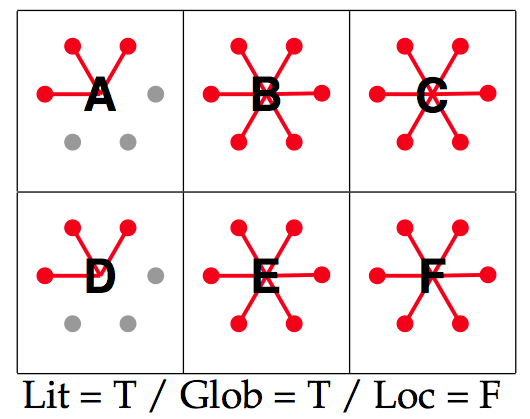
\includegraphics[scale=0.25]{../pictures/paper/Chemla_Spector_2010_Critical_AE.png}\\
      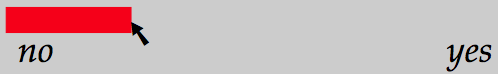
\includegraphics[scale=0.25]{../pictures/paper/Chemla_Spector_2010_RatingBar.png}
    \end{center}

  \end{minipage}
    }
   \begin{minipage}{6cm}
     \subfloat[][Results \as-condition]{
    \label{fig:CS-Results-as}
        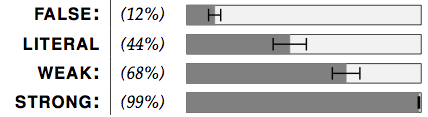
\includegraphics[width=5.5cm]{../pictures/paper/Chemla_Spector_2010_Results_AE.png}
  }

  \subfloat[test][Results \es-condition]{
    \label{fig:CS-Results-es}
    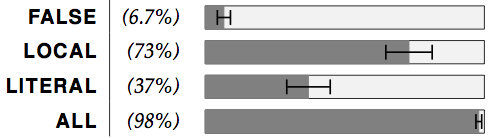
\includegraphics[width=5.5cm]{../pictures/paper/Chemla_Spector_2010_Results_GE.png}
  }  
   \end{minipage}
        \caption{Example trial and results of
          \citeauthor{ChemlaSpector2010:Experimental-Ev}'s
          (\citeyear{ChemlaSpector2010:Experimental-Ev}) study.}
\end{figure}

% \begin{figure}[t]
%   \centering
%       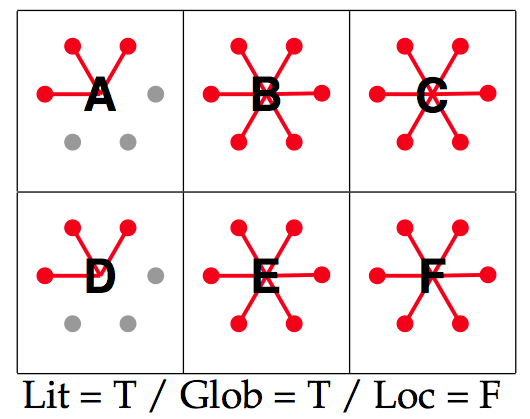
\includegraphics[scale=0.25]{../pictures/paper/Chemla_Spector_2010_Critical_AE.png}\\
%       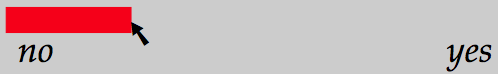
\includegraphics[scale=0.25]{../pictures/paper/Chemla_Spector_2010_RatingBar.png}
%         \caption{Example of critical trial for \as-condition by
%           \citeauthor{ChemlaSpector2010:Experimental-Ev}'s
%           (\citeyear{ChemlaSpector2010:Experimental-Ev})}
%   \label{fig:Chemla-Spector}
% \end{figure}

\citeauthor{ChemlaSpector2010:Experimental-Ev} hypothesized that the
degree to which a sentence is rated acceptable is proportional to the
number of available true readings. Observed averaged clicking
positions are shown in Figures~\ref{fig:CS-Results-as} and
\ref{fig:CS-Results-es}.
%
% \begin{figure}
%   \centering
%   \subfloat[][\as-condition]{
%     \label{fig:CS-Results-as}
%         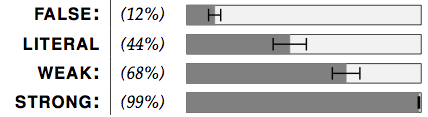
\includegraphics[width=5.5cm]{../pictures/paper/Chemla_Spector_2010_Results_AE.png}
%   }
%   \subfloat[test][\es-condition]{
%     \label{fig:CS-Results-es}
%     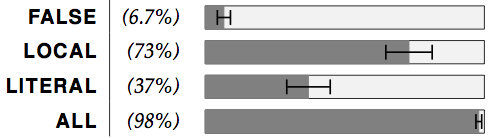
\includegraphics[width=5.5cm]{../pictures/paper/Chemla_Spector_2010_Results_GE.png}
%   }
%   \caption{Results from
%     \citeauthor{ChemlaSpector2010:Experimental-Ev}'s
%     (\citeyear{ChemlaSpector2010:Experimental-Ev}) study}
%   \label{fig:Chemla-Spector-Results}
% \end{figure}
%
According to \citeauthor{ChemlaSpector2010:Experimental-Ev}, the
crucial piece of evidence for the availability of local readings for
\as-sentences is that these sentences yielded higher graded
acceptability scores for the strong situation than for the weak
situation (although these differ only with respect to the truth value
of the local reading). Evidence for the availability
of the local reading for \es-sentences comes from the difference
between the local and the literal situation. Strikingly, \es-sentences
received an average 73\% degree of acceptability in the local
situation although the literal and global readings are false in this
case.

\subsection{Reflection}
\label{sec:local-read-categ}

Summing up, three experimental studies have presented diverging pieces
of evidence. % \citet{GeurtsPouscoulous2009:Embedded-Implic} did not
% observe any truth value-judgments that would indicate local readings
% in a picture verification task and thus conclude that these readings
% are unavailable. \citet{CliftonDube2010:Embedded-Implic} and
% \citet{ChemlaSpector2010:Experimental-Ev} employed different designs
% intended to be sensitive enough to reveal local readings. Both studies
% found putative evidence in support of local readings.
Differences in results are likely due to differences in experimental
design, in particular due to (i) the type of elicited judgement and
(ii) the possibility of conflating pictorial effects.

\paragraph{Judgement Type.} We could draw a distinction between
\emph{categorical} truth-value judgments and other more sensitive
measures. The former are possibly not sensitive enough to reveal
dispreferred readings with small samples, but the latter may be. We
could then hypothesize along with
\citeauthor{CliftonDube2010:Embedded-Implic} and
\citeauthor{ChemlaSpector2010:Experimental-Ev} that local readings are
available, but so dispreferred that they do not affect categorical
truth-value judgments. 

On the other hand, \citet{Crain1998} argue in favor of truth-value
judgments as a means of detecting dispreferred readings. Consequently,
traditionalists could reply that the putative evidence for local
readings in non-categorical judgement tasks might reflect something
other than (strongly) truth-relevant speaker-intended meaning
enrichments. Hence no case can be made for lexicalism or
grammaticalism on the basis of these data \citep[see][for arguments
along these
lines]{GeurtsTielvan-Tiel2013:Scalar-expressi,Tielvan-Tiel2014:Quantity-Matter,Tielvan-Tiel2012:Embedded-Scalar}.

To resolve this issue, we would ideally like to have a design that
elicits categorical judgements, but is still possibly sensitive enough
to detect dispreferred readings. 

\paragraph{Pictorial Effects.} Choice of pictorial material can have
an effect on obtained results \citep[see][for related
discussion]{Raffray2010}. It is often possible to present different
numbers of links between icons in pictures like in
Figures~\ref{fig:AS-distinguishing-pics}
and~\ref{fig:ES-distinguishing-pics}, without changing the
truth-values of relevant readings. Indeed, the pictorial material used
in previous studies differed in this respect, and that might explain
some of the differences in results.

If that is so, then we cannot ascribe the effects reported by
\citet{CliftonDube2010:Embedded-Implic} and
\citet{ChemlaSpector2010:Experimental-Ev} to the availability of local
readings with certainty. \citet{ChemlaSpector2010:Experimental-Ev}
also acknowledge the possibility that the \emph{typicality} of a
picture with respect to some meaning may affect graded truth-value
judgments. They show that graded judgments of \as-sentences differ
significantly for different pictures that agree on the truth value of
relevant readings but differ with respect to the amount of connections
between icons. \citeauthor{ChemlaSpector2010:Experimental-Ev} suggest
that typicality of the pictorial material can account for these
differences, but submit that this does not explain away the high
acceptance of pictures like Figure \ref{fig:weak}. The latter point is
disputed by \citet{Tielvan-Tiel2012:Embedded-Scalar}, who demonstrates
that a huge chunk of variance in the responses to \as-sentences can be
explained as typicality effects, dispensing the need to appeal to the
distribution of different readings. In support of this idea,
\citet{Tielvan-Tiel2012:Embedded-Scalar} elicited what he calls the
typicality structures associated with the quantifiers {\it all} and
{\it some} \citep[as done also
by][]{DegenTanenhaus2011:Making-Inferenc} and predicted the judgments
of \as-sentences obtained by
\citeauthor{ChemlaSpector2010:Experimental-Ev} based on these
data. Thereby, he obtained an excellent model fit.

We are generally sympathetic towards
\citeauthor{Tielvan-Tiel2012:Embedded-Scalar}'s innovative line of
reinterpretation of the data, but note, as
\citet{ChemlaSpector2010:Experimental-Ev} already observed, that his
typicality-based explanation does not extend to \es-sentences in an
obvious way. Moreover, typicality itself is not a satisfactory
primitive in a putative explanation of the use of quantifiers. Rather
it is possible to explain typicality judgements as the outcome of
Gricean speaker preferences for informative descriptions, just like
those that rationalize quantity implicatures
\citep{Franke2014:Typical-use-of-}. For these reasons, we believe that
typicality and other pictorial effects need to be taken seriously in
the experimental design, but do not give a satisfactory account of the
observed variation all by themselves.

\paragraph{Upshot.} Taken together, we would ideally like a design
that evokes categorical truth value judgments in a way that is as
independent as possible of potentially conflating properties of the
pictorial material and that is nonetheless sensitive enough to detect
local readings even if they are dispreferred. The sensitivity to
dispreferred readings should be controlled for. On top of this, it
would be desirable to obtain further information about the relative
preferences among all putative readings, so as to be able to decide
between theoretical positions, as outlined in
Section~\ref{sec:theories-predictions}. % Neither of the previous
% studies gives us that, either because they simply have not
% investigated all the relevant comparisons
% (\citet{GeurtsPouscoulous2009:Embedded-Implic},
% \citet{CliftonDube2010:Embedded-Implic}), or because they cannot
% safely derive the required information for danger of conflating
% preferences for readings with preferences for pictures
% (\citet{ChemlaSpector2010:Experimental-Ev}).

Finally, we need to control for ``silent prosody.'' A growing number
of evidence suggests that numerous factors might influence accent
placement and prosodic phrasing even while reading, amongst them
default accentuation, constituent length, rhythmic phenomena, and
individual variation
\citep[e.g.][]{Augurzky08,Bader98,Fodor98,Fodor02,Kentner12,
  Steinhauer01}. If we adopt the intonational markedness hypothesis
described in Section~\ref{sec:inton-mark-hypoth}, as many
traditionalists do, we predict that the availability of a local
reading hinges on the realization of contrastive stress on the scalar
item
\citep[e.g.][]{Horn2006:The-Border-Wars,Geurts2009:Scalar-Implicat,Geurts2010:Quantity-Implic,Tielvan-Tiel2012:Embedded-Scalar,GeurtsTielvan-Tiel2013:Scalar-expressi}.
But if intonation can have this role, it is necessary to control for
silent accent placement. Ideally, therefore, we should present
sentences auditorily and manipulate contrastive stress systematically.


\section{An Incremental Verification Task}
\label{sec:exp}

\subsection{Design}
\label{sec:design}

\paragraph{General Idea.} In order to test the availability and
preferences of different readings of \as- and \es-sentences in German,
we were looking for a way to unambiguously map responses from a
picture verification task to specific readings. We were particularly
interested in the question whether local readings would be observed at
all, and whether their presence or absence would be modulated by a
contrastive accent on the scalar item. Moreover, we were interested in
obtaining information about the relative preferences of the different
readings. In addition, we wanted to minimize potential picture
typicality effects. To achieve this, we used an \mymark{incremental
  verification task} (\acro{ivt}), which is a modified version of
picture verification \citep[see][]{Conroy2008}. The general idea is
that subjects are requested to judge sentence material based on
pictures that do not necessarily contain all the information necessary
to judge a certain reading true or false. In that case, participants
can demand that more information be revealed. Participants are
instructed to make a truth-value judgment as soon as they are able
to. When they do, the trial ends.

\paragraph{Target Conditions.} We present sequences of pictures
depicting a set of four identical central elements (e.g., letters),
which could be connected to surrounding elements (e.g., triangles), as
shown in Figures~\ref{fig:exseqAS}--\ref{fig:exec}. Initially,
any potential connections between central and surrounding elements
were covered by dark gray color (see
Figure~\ref{fig:exseqAS1}). Sentences to be judged were presented
auditorily, and participants were asked to uncover the picture until
they felt able to give a truth value judgment. Three options were
available for participants at each step: (i) judge the sentence as
true, (ii) judge the sentence as false, (iii) demand more information
(unavailable when the picture was fully uncovered). Trials ended when
a truth-value judgement was made. Importantly, each of the three
potentially available readings corresponded to a specific step in the
uncovering process where the truth value of that reading (and only of
that reading) could be assessed for the first time. We refer to this
step in the sequence as the {\it critical position} of a given
reading. The critical position and the corresponding truth-value
judgment differed between \as- and \es-sentences, as described
presently. (This is, partly, because of the logical dependencies
between readings, and, partly, also to rule out positional biases.)

\begin{figure}[]
	\centering
	\subfloat[][Step 1]{ 
		\fbox{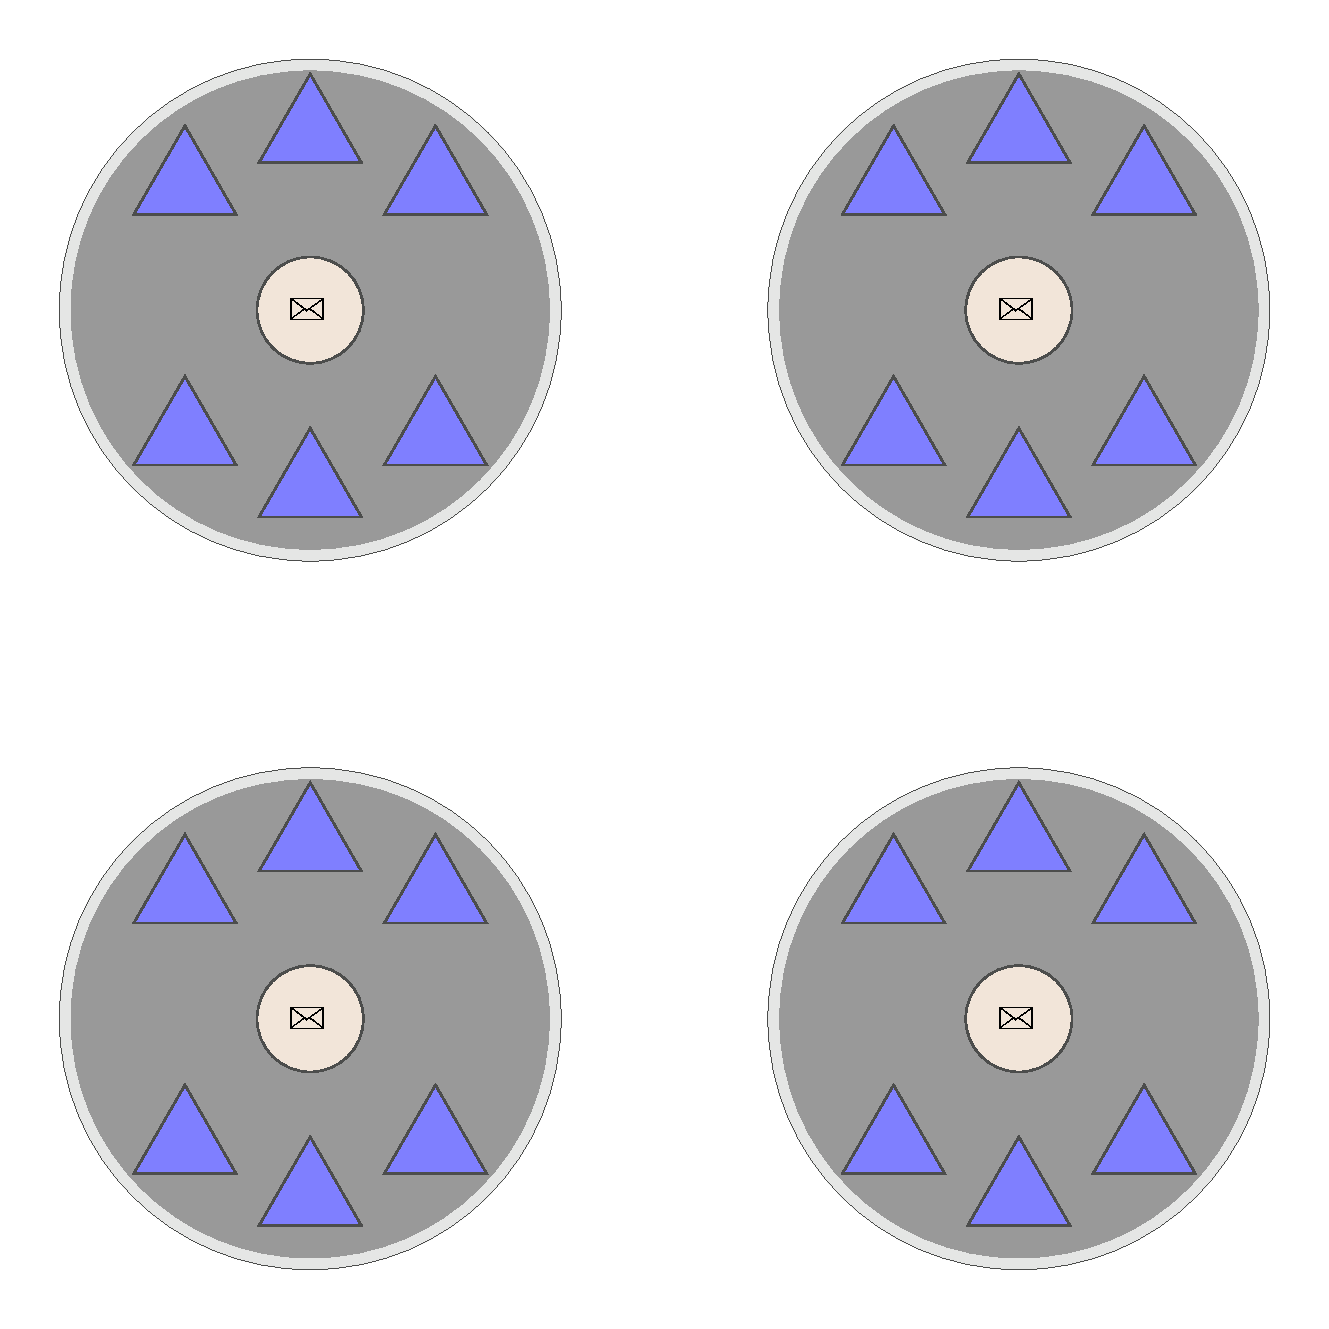
\includegraphics[width=3.5cm]{../pictures/ae_01_1.pdf}}
	    \label{fig:exseqAS1}
	}
	\subfloat[][Step 2]{
		\fbox{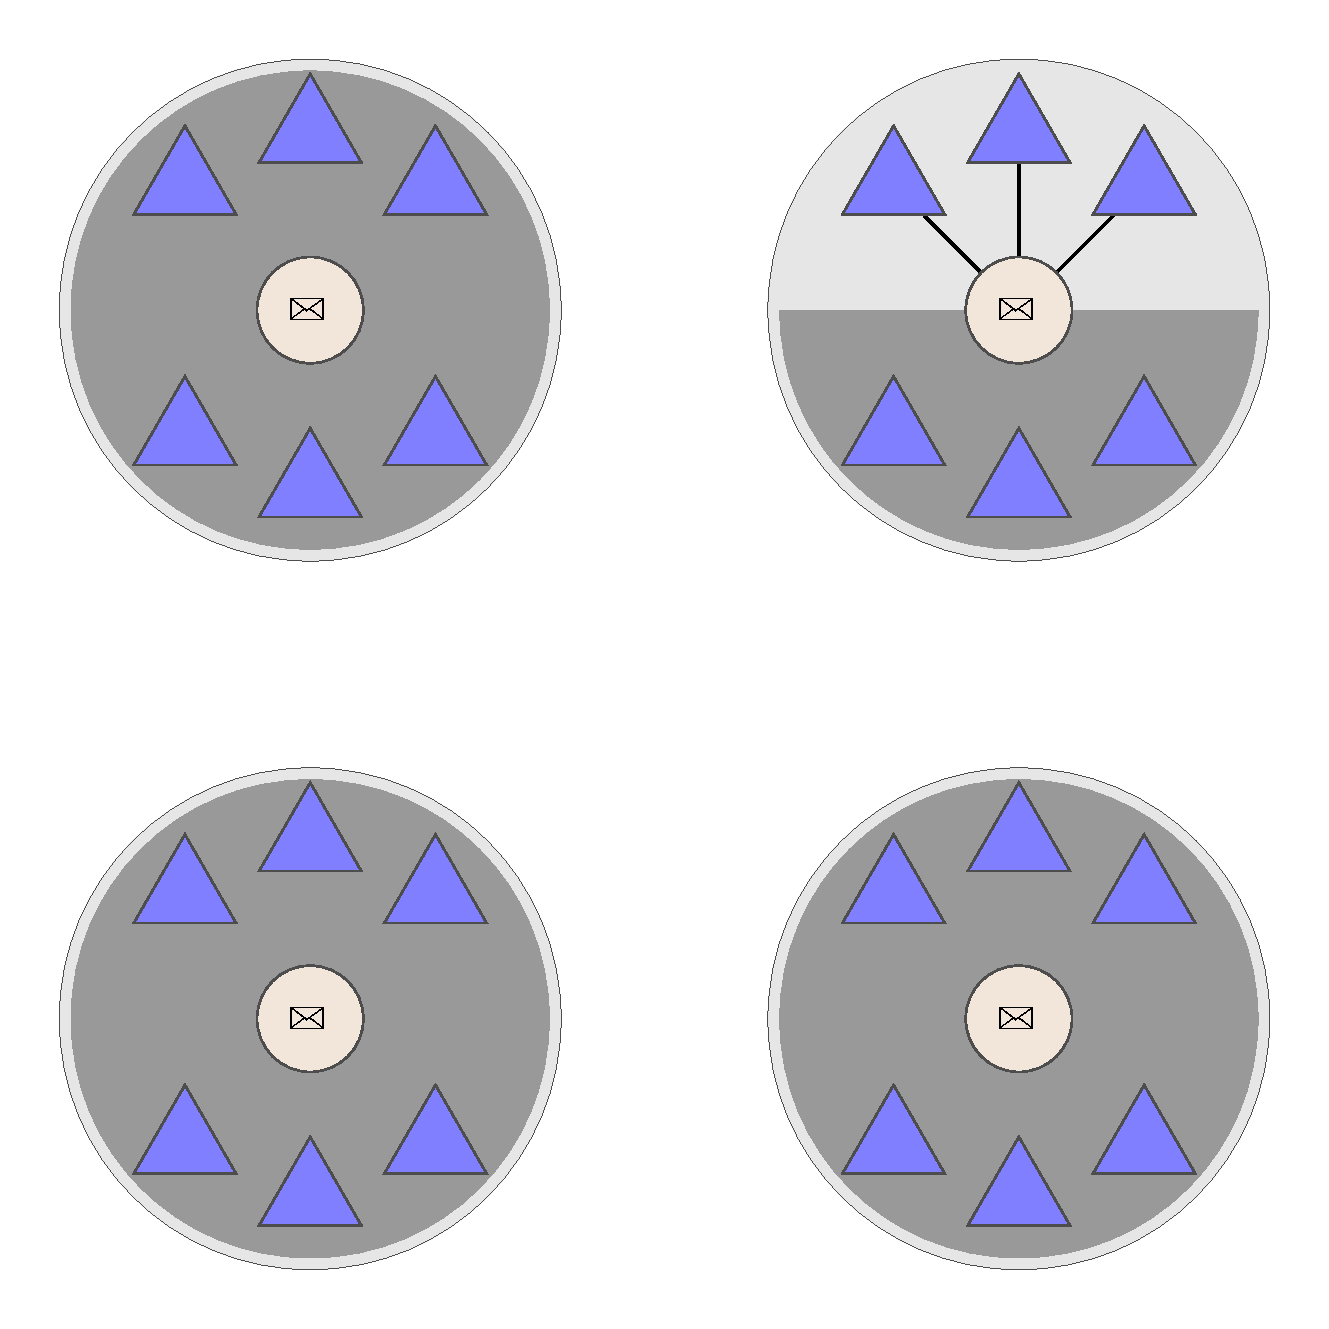
\includegraphics[width=3.5cm]{../pictures/ae_01_2.pdf}}
	    \label{fig:exseqAS2}
	}
	\subfloat[][Step 3 (\lit true)]{ 
		\fbox{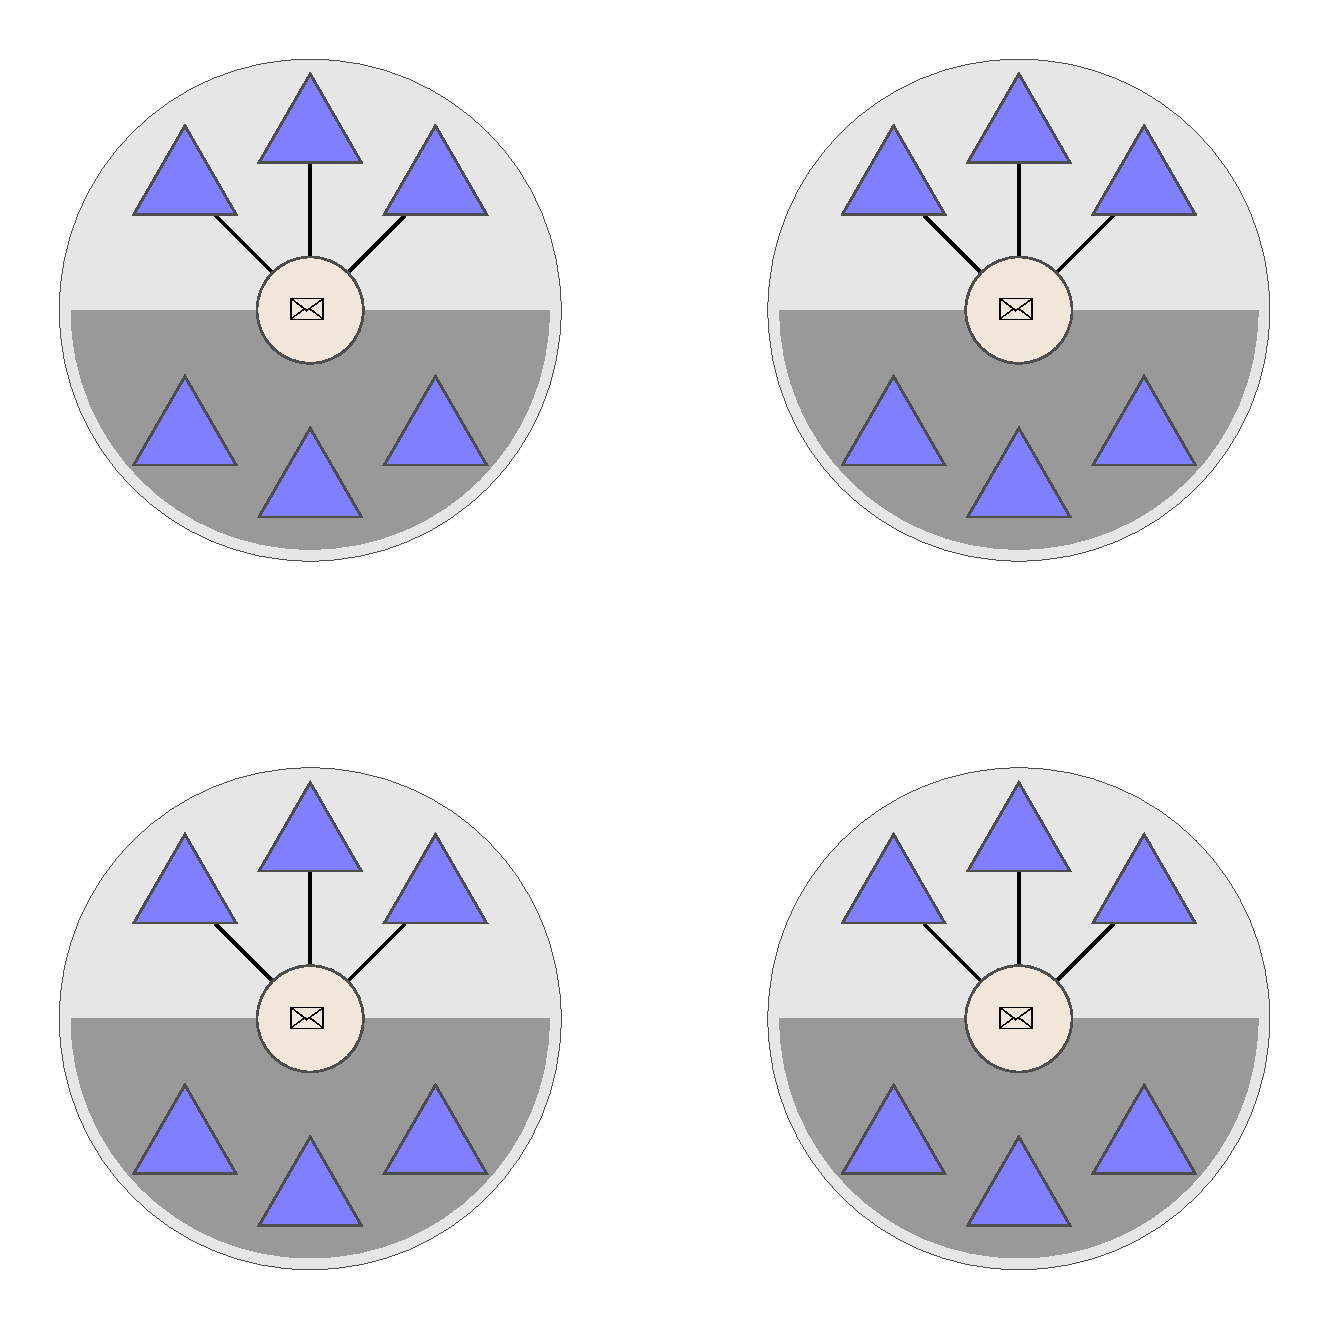
\includegraphics[width=3.5cm]{../pictures/ae_01_3.pdf}}
	    \label{fig:exseqAS3}
	}
        \\
	\subfloat[][Step 4]{ 
		\fbox{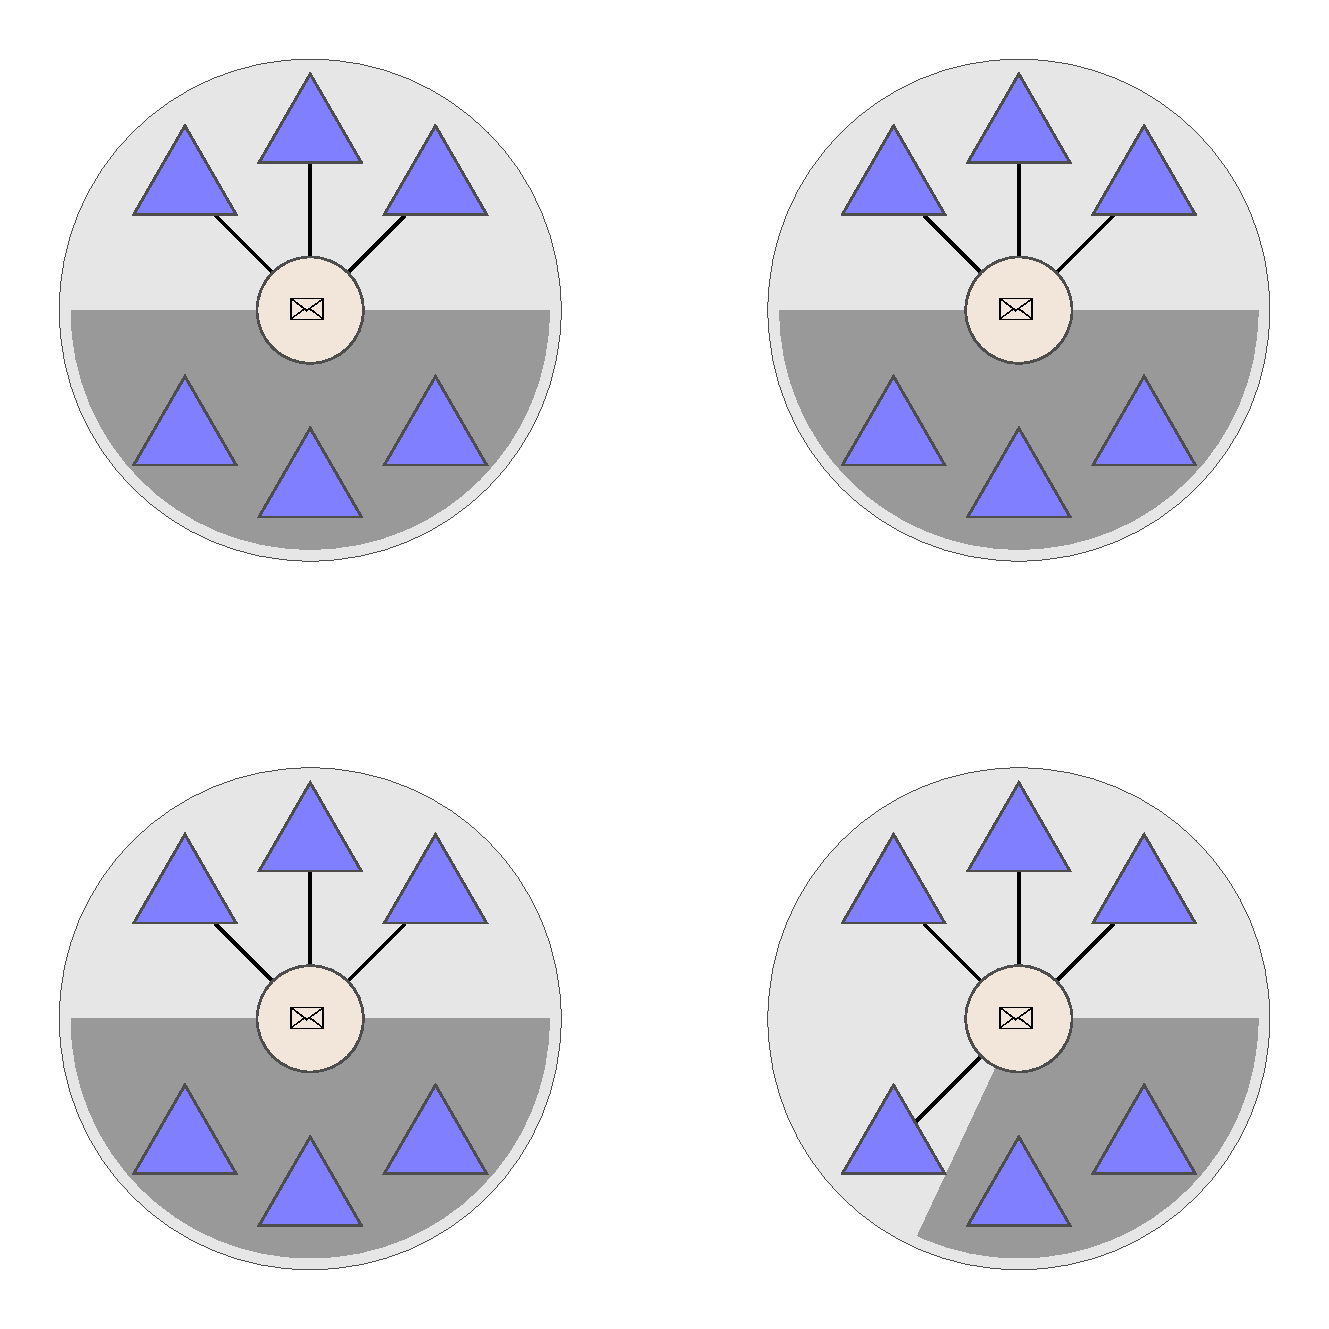
\includegraphics[width=3.5cm]{../pictures/ae_01_4.pdf}}
	    \label{fig:exseqAS4}
	}
	\subfloat[][Step 5 (\glb true)]{
		\fbox{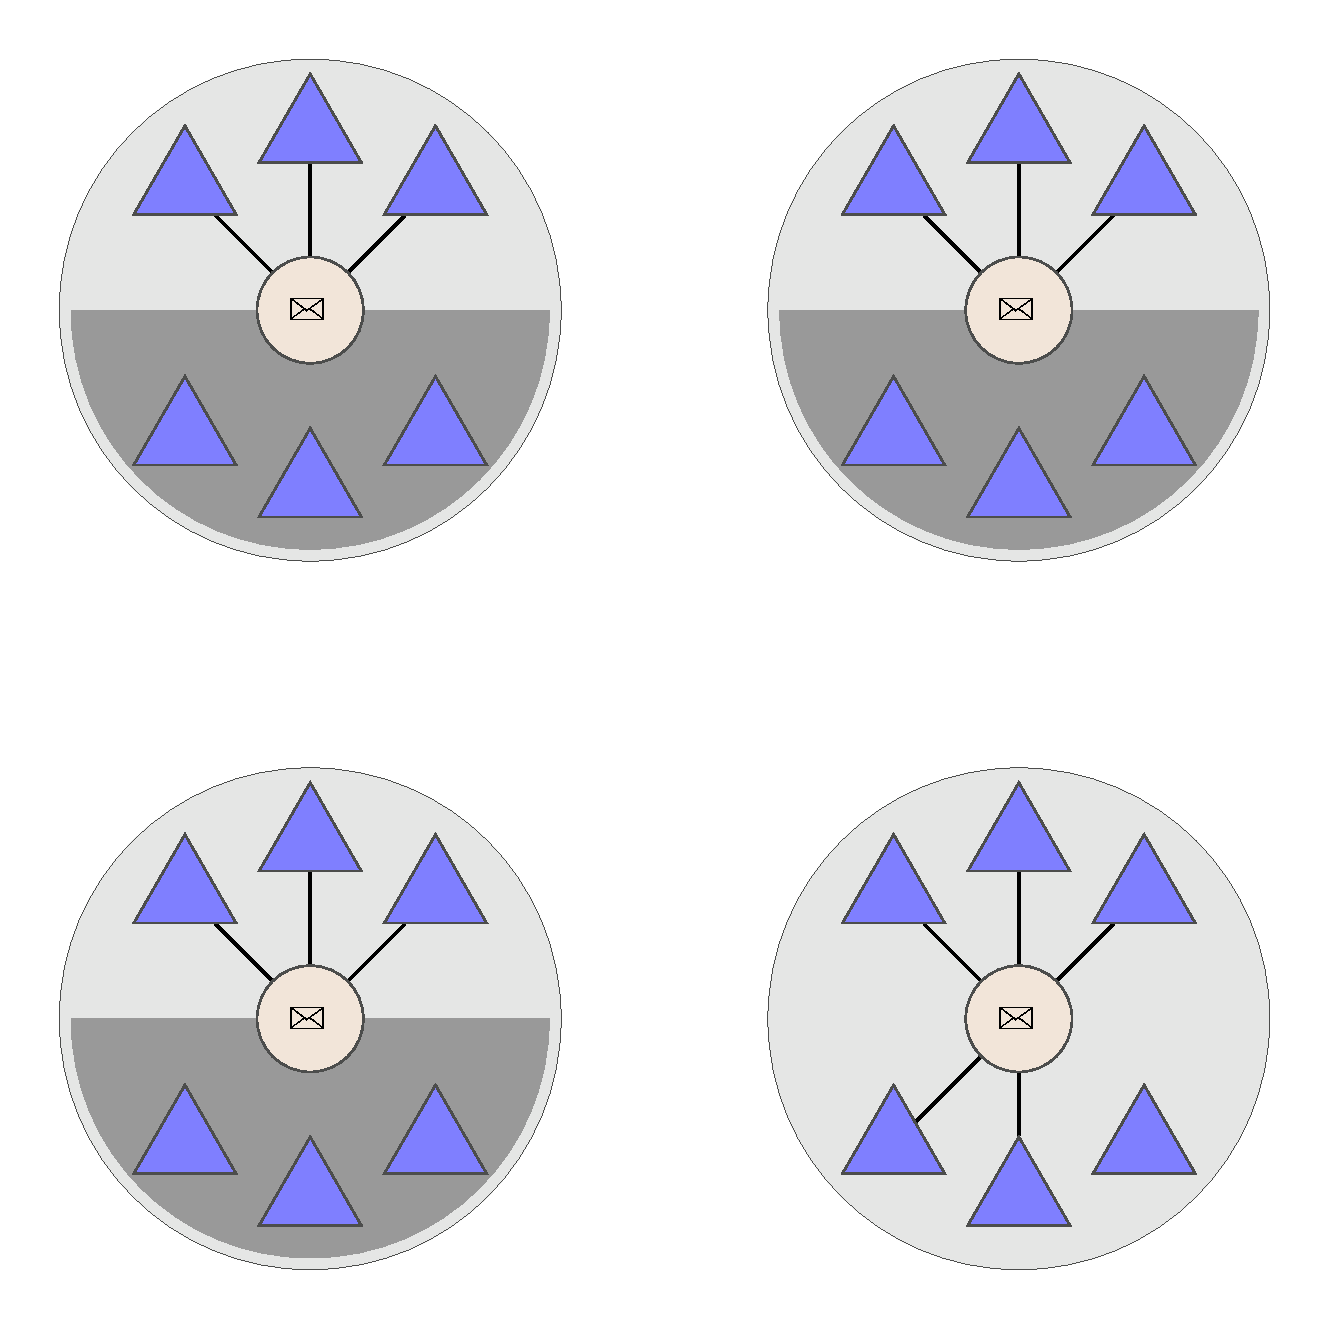
\includegraphics[width=3.5cm]{../pictures/ae_01_5.pdf}}
	    \label{fig:exseqAS5}
	}
	\subfloat[][Step 6]{ 
		\fbox{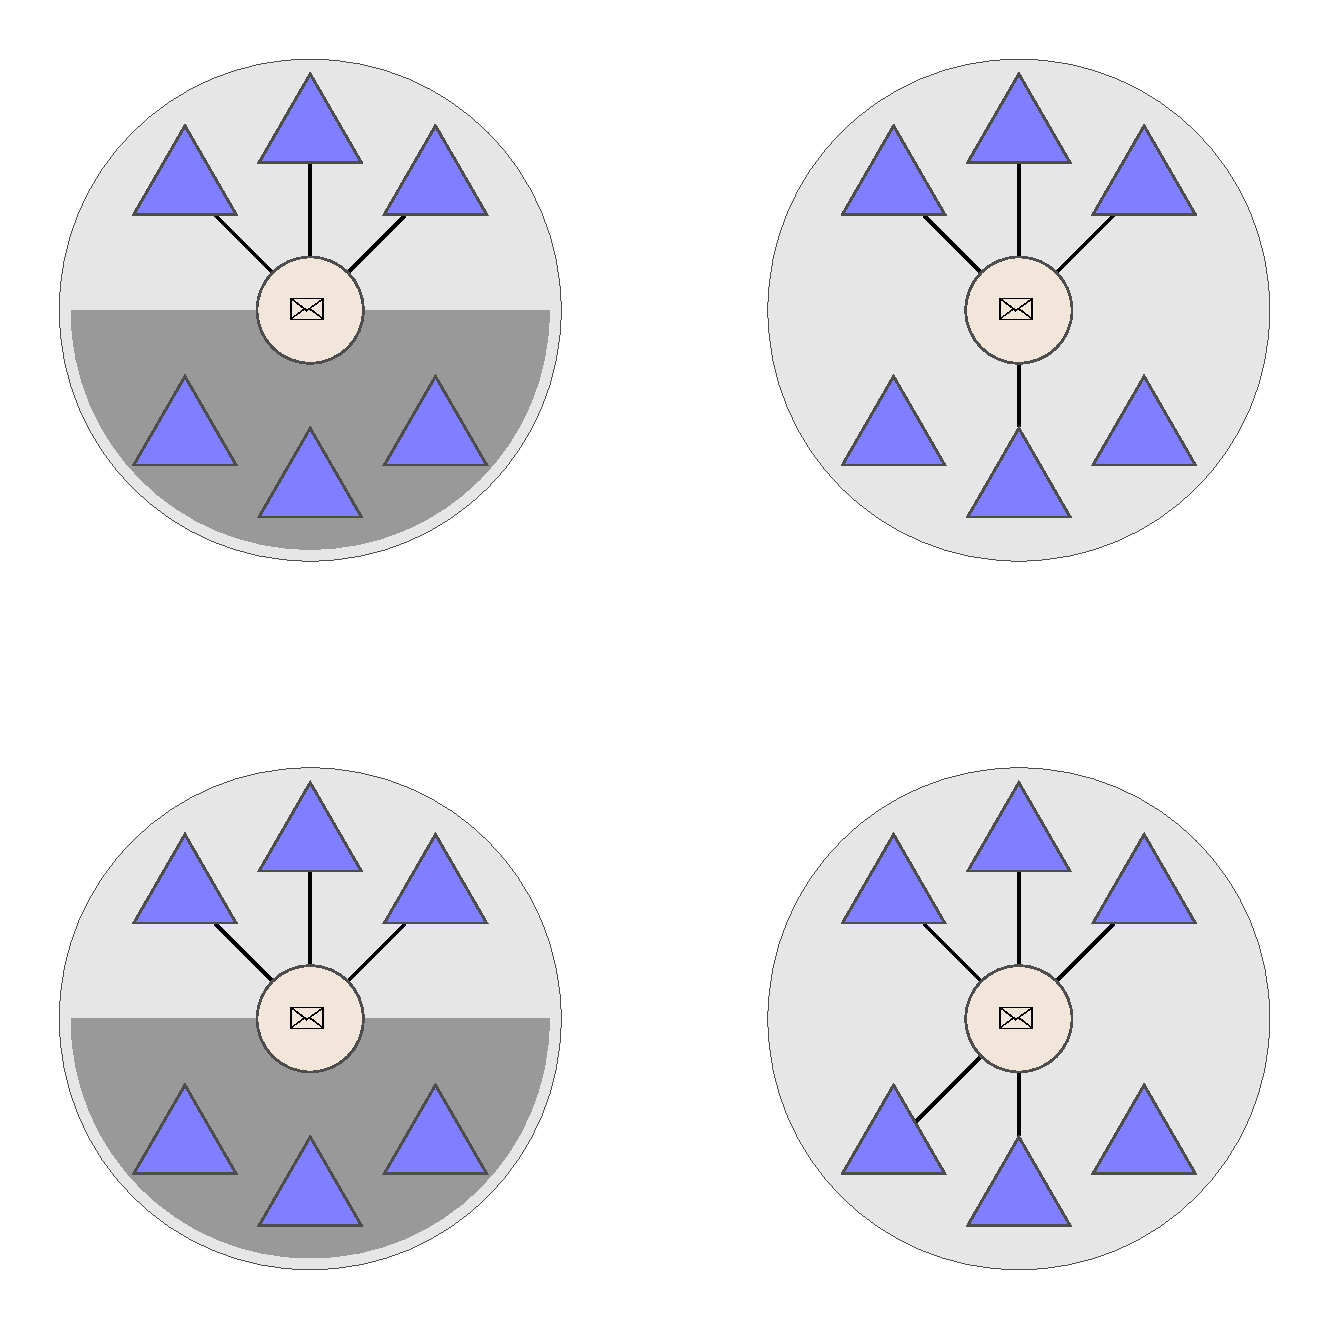
\includegraphics[width=3.5cm]{../pictures/ae_01_6.pdf}}
	    \label{fig:exseqAS6}
	}
        \\
	\subfloat[][Step 7 (\loc false)]{ 
		\fbox{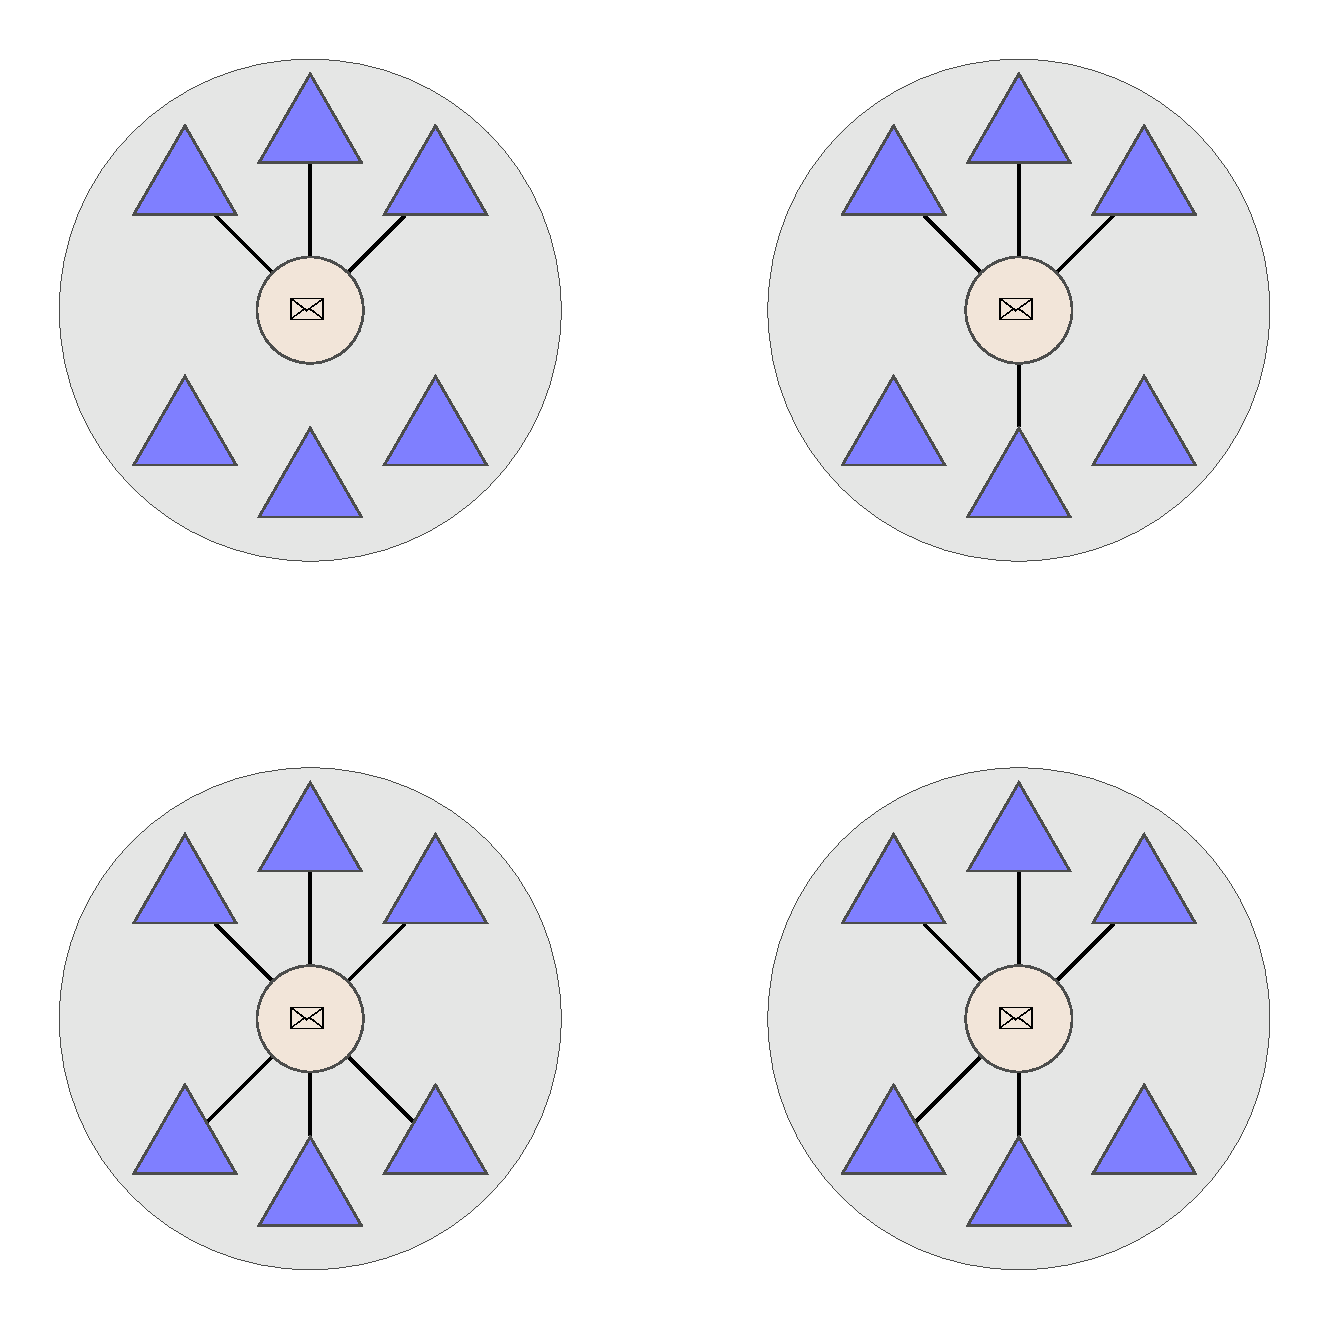
\includegraphics[width=3.5cm]{../pictures/ae_01_7.pdf}}
	    \label{fig:exseqAS7}
	} 
                \hspace*{7.85cm} 
	\caption[]{Example picture sequence for \as-sentences.}
	\label{fig:exseqAS}
\end{figure}


Consider the German \as-sentence in (\ref{ex:as}), included in our study.
\begin{exe}
\ex \gll \mymark{Alle} diese Briefe sind mit \mymark{einigen} ihrer Dreiecke
  verbunden.\label{ex:as}\\
All these letters are with some their triangles connected.\\
\trans All of these letters are connected to some of their triangles.
\end{exe}
Figure~\ref{fig:exseqAS} shows the corresponding picture sequence. The
critical positions are on step 3, 5 and 7. Pictures that were
interspersed between these positions served as
spillover-pictures. These were used in order to control for
potentially delayed judgments and they additionally served as
distractor items. Prior to step 3 there is not enough information to
judge any candiate reading true or false. The situation at step 3 in
Figure~\ref{fig:exseqAS3} is true under a literal reading, while the
local and global readings cannot be evaluated yet. On step 5 in
Figure~\ref{fig:exseqAS5} the literal reading is still true, but now
also the global reading can be confirmed. Finally, decisions
concerning the local reading are possible as soon as all connections
have been uncovered at step 7 in Figure~\ref{fig:exseqAS7}. Note that
the situation at step 7 is \emph{in}compatible with a local
reading. This enables us to separate local readings, which would yield
\emph{false} judgements at this position, from literal and global
readings, which would yield \emph{true} judgements. In sum,
\emph{true} or \emph{false} answers on particular positions in the
incrementally revealed picture sequence can be mapped uniquely to
candidate readings. All other \emph{true} or \emph{false} answers were
counted as errors.

\es-sentences, due to the non-linear relationship of readings
described in Section~\ref{sec:get-know-your}, require a slightly
different sequence of unfolding which yields a different order in
which truth-value judgments can be made.
%
\begin{figure}[t]
	\centering
	\subfloat[][Step 1]{ 
		\fbox{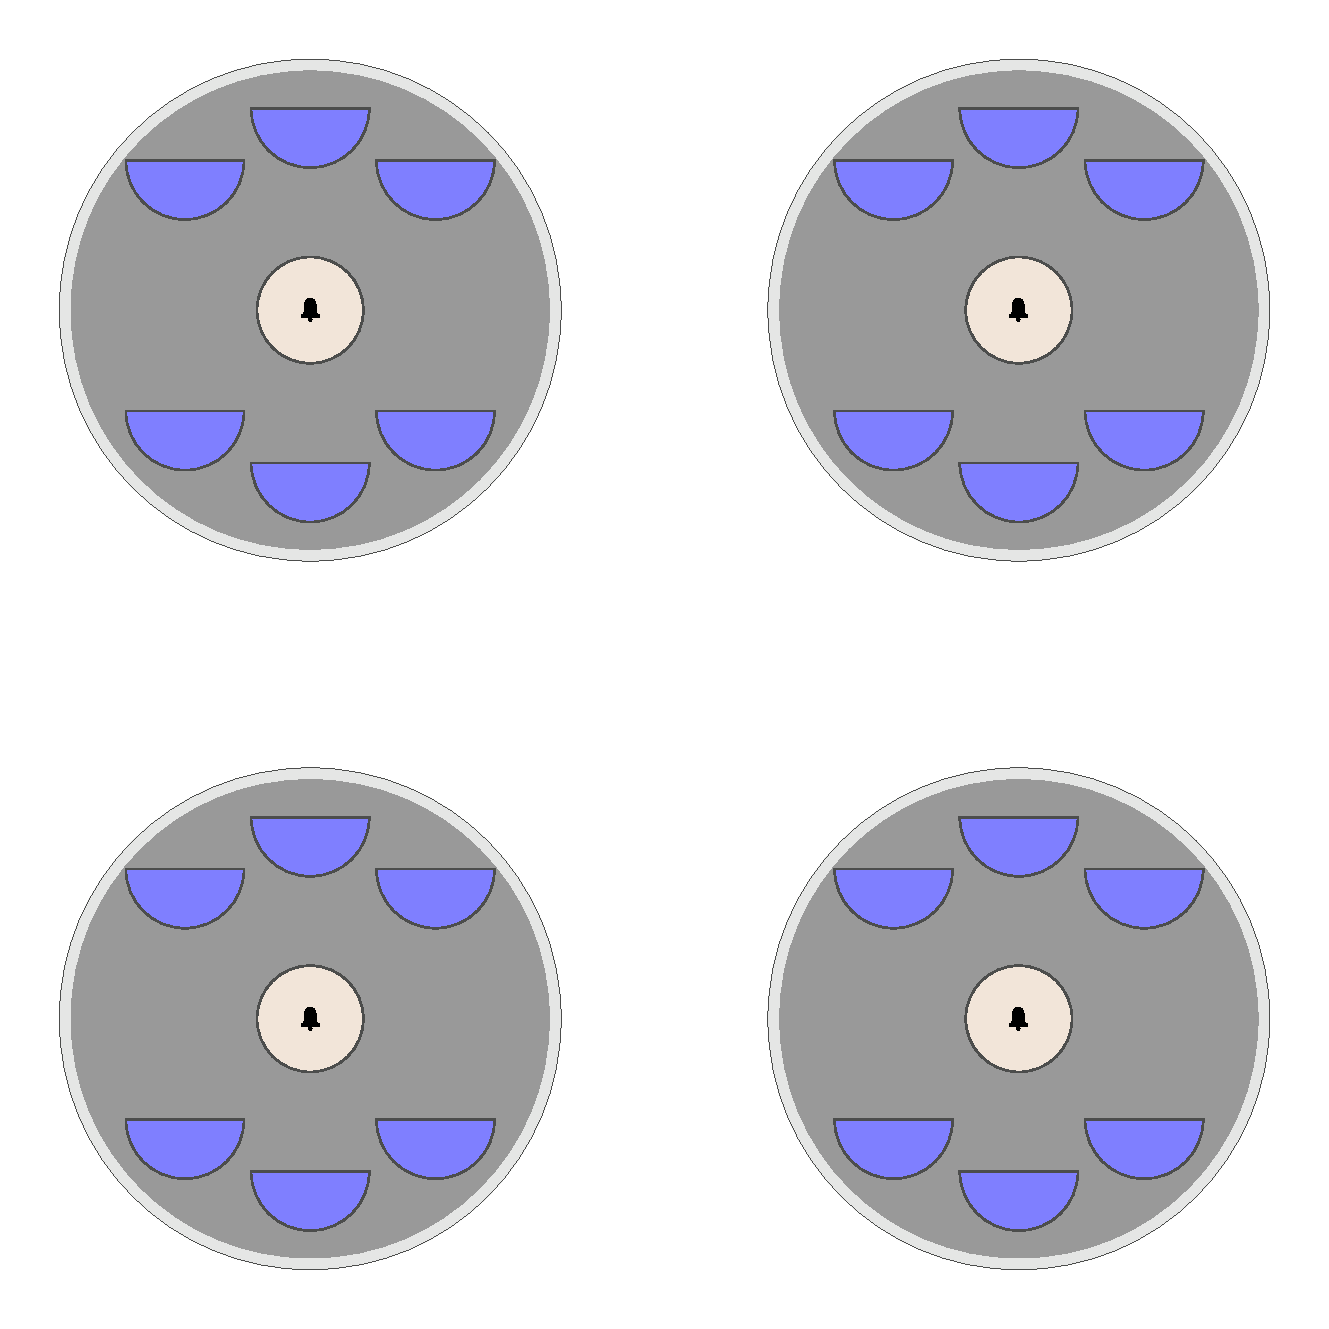
\includegraphics[width=3.5cm]{../pictures/ge_01_1.pdf}}
	    \label{fig:exseqES1}
	}
	\subfloat[][Step 2 (\glb false)]{
		\fbox{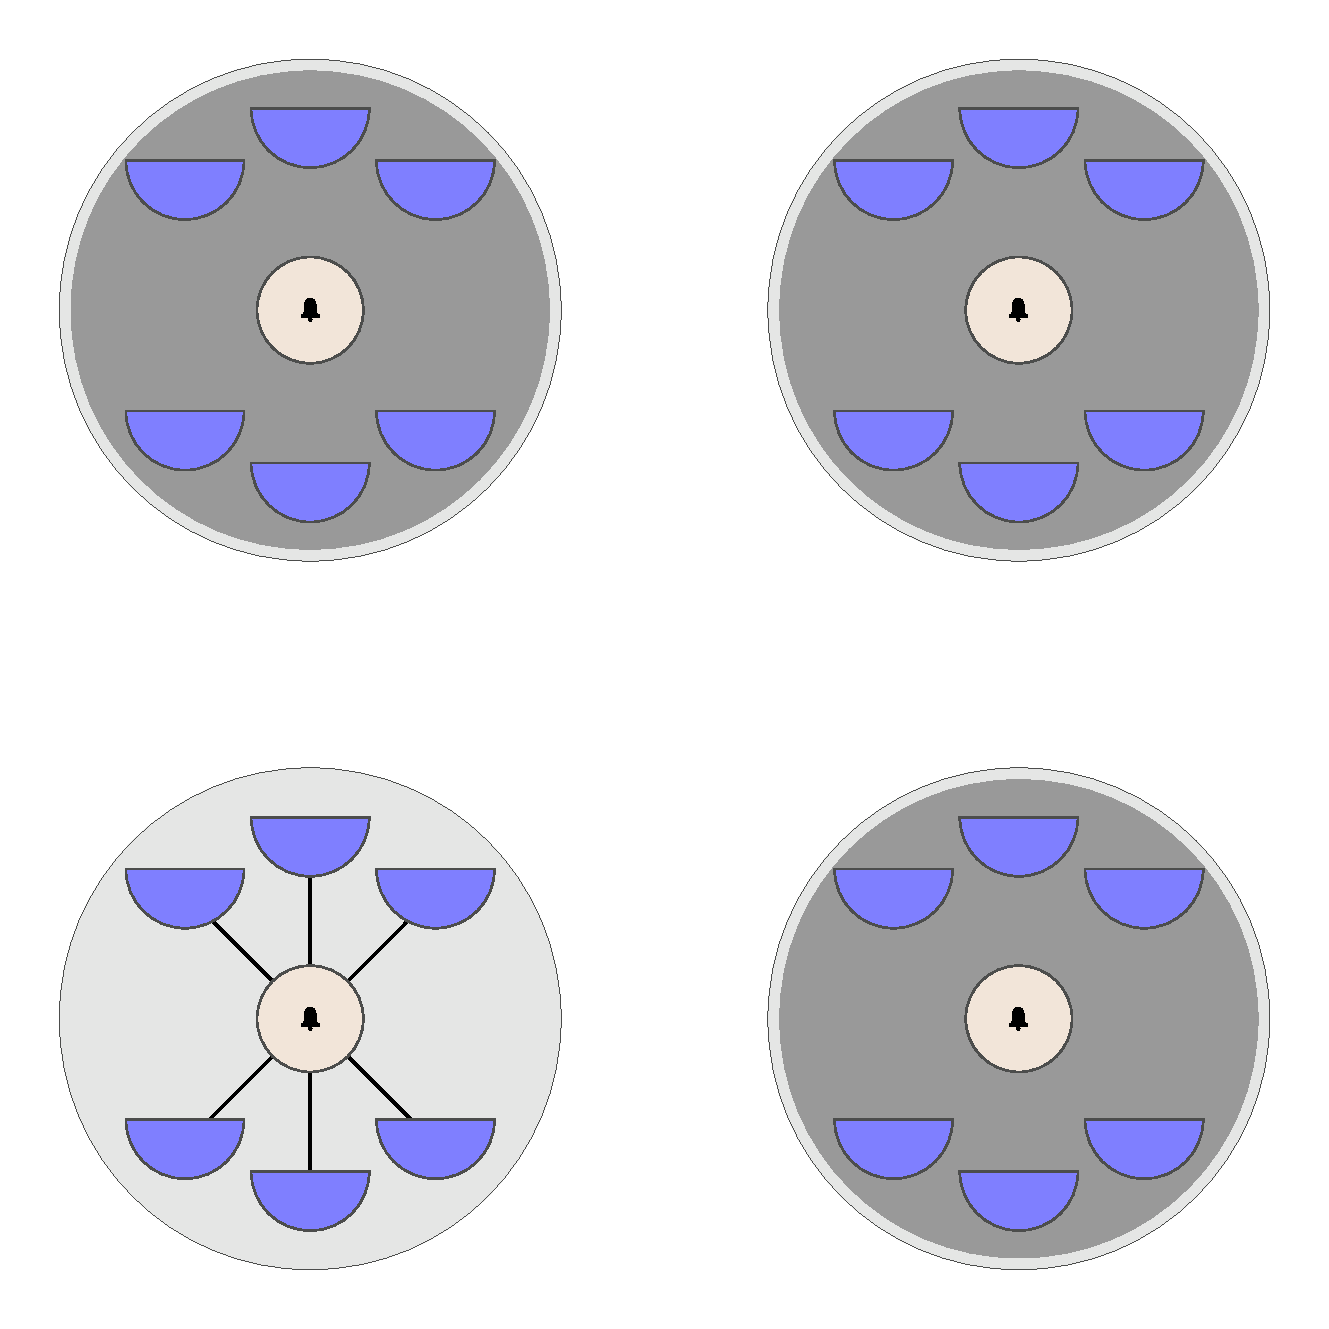
\includegraphics[width=3.5cm]{../pictures/ge_01_2.pdf}}
	    \label{fig:exseqES2}
	}
	\subfloat[][Step 3 (\lit false)]{ 
		\fbox{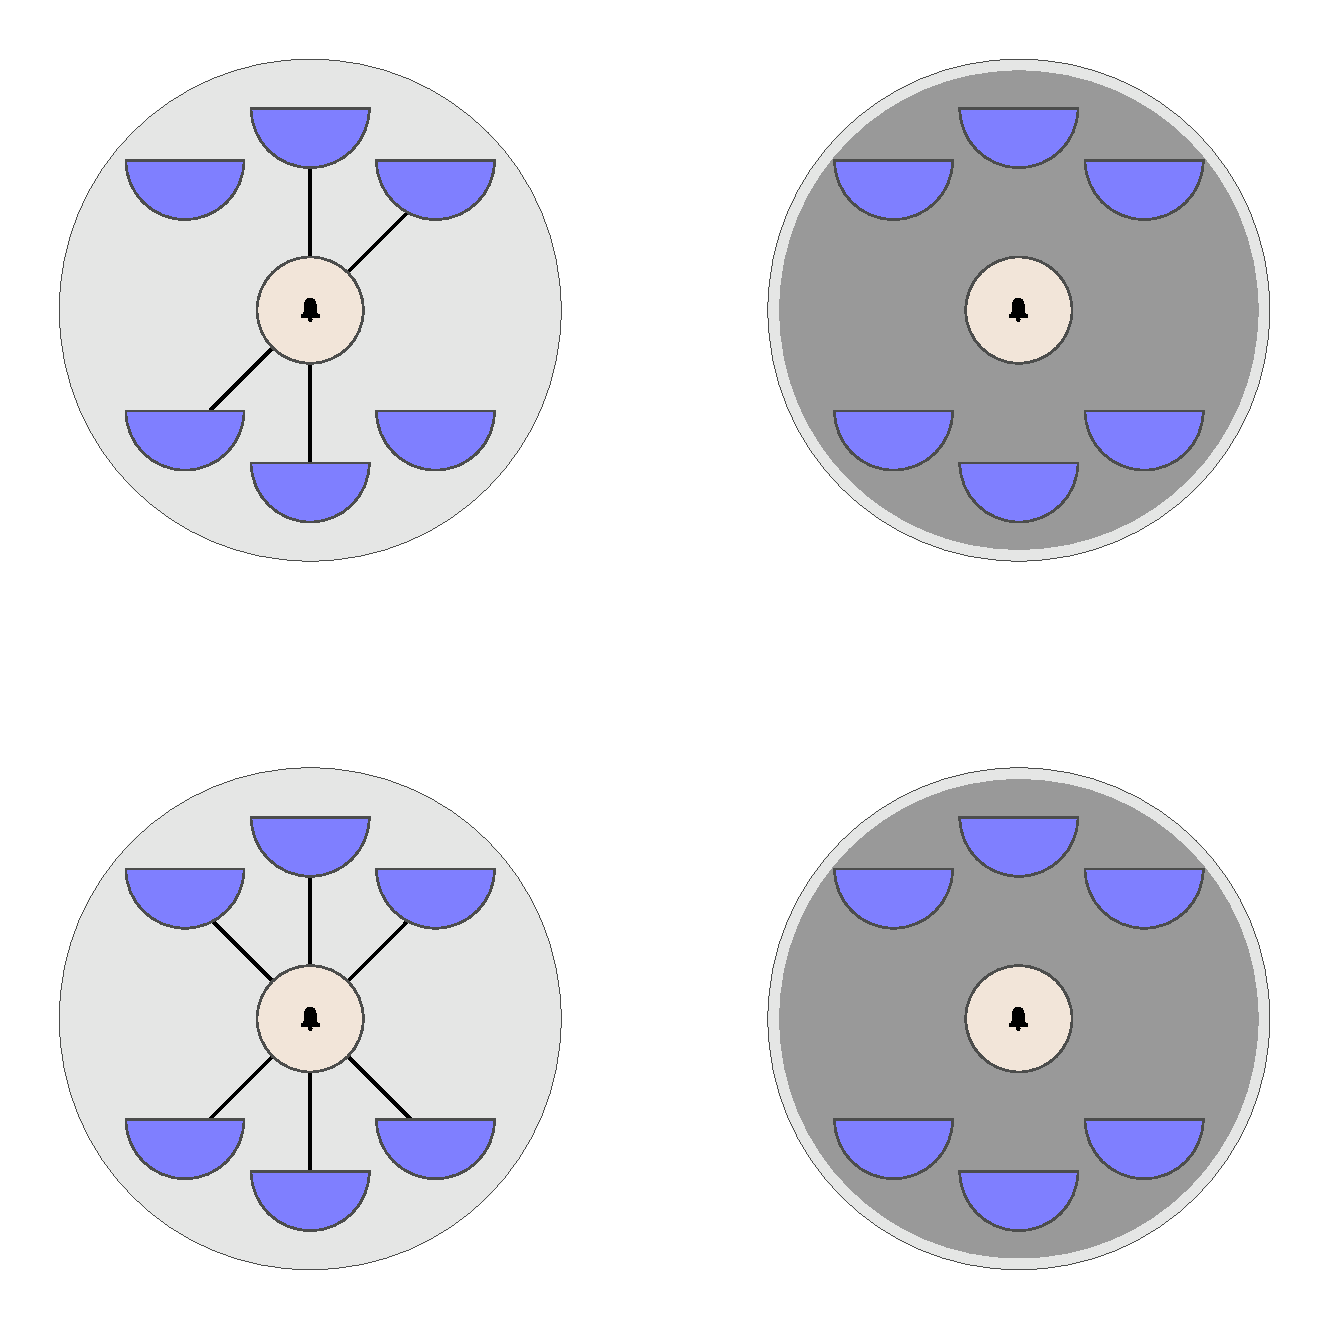
\includegraphics[width=3.5cm]{../pictures/ge_01_3.pdf}}
	    \label{fig:exseqES3}
	}
        \\
	\subfloat[][Step 4]{ 
		\fbox{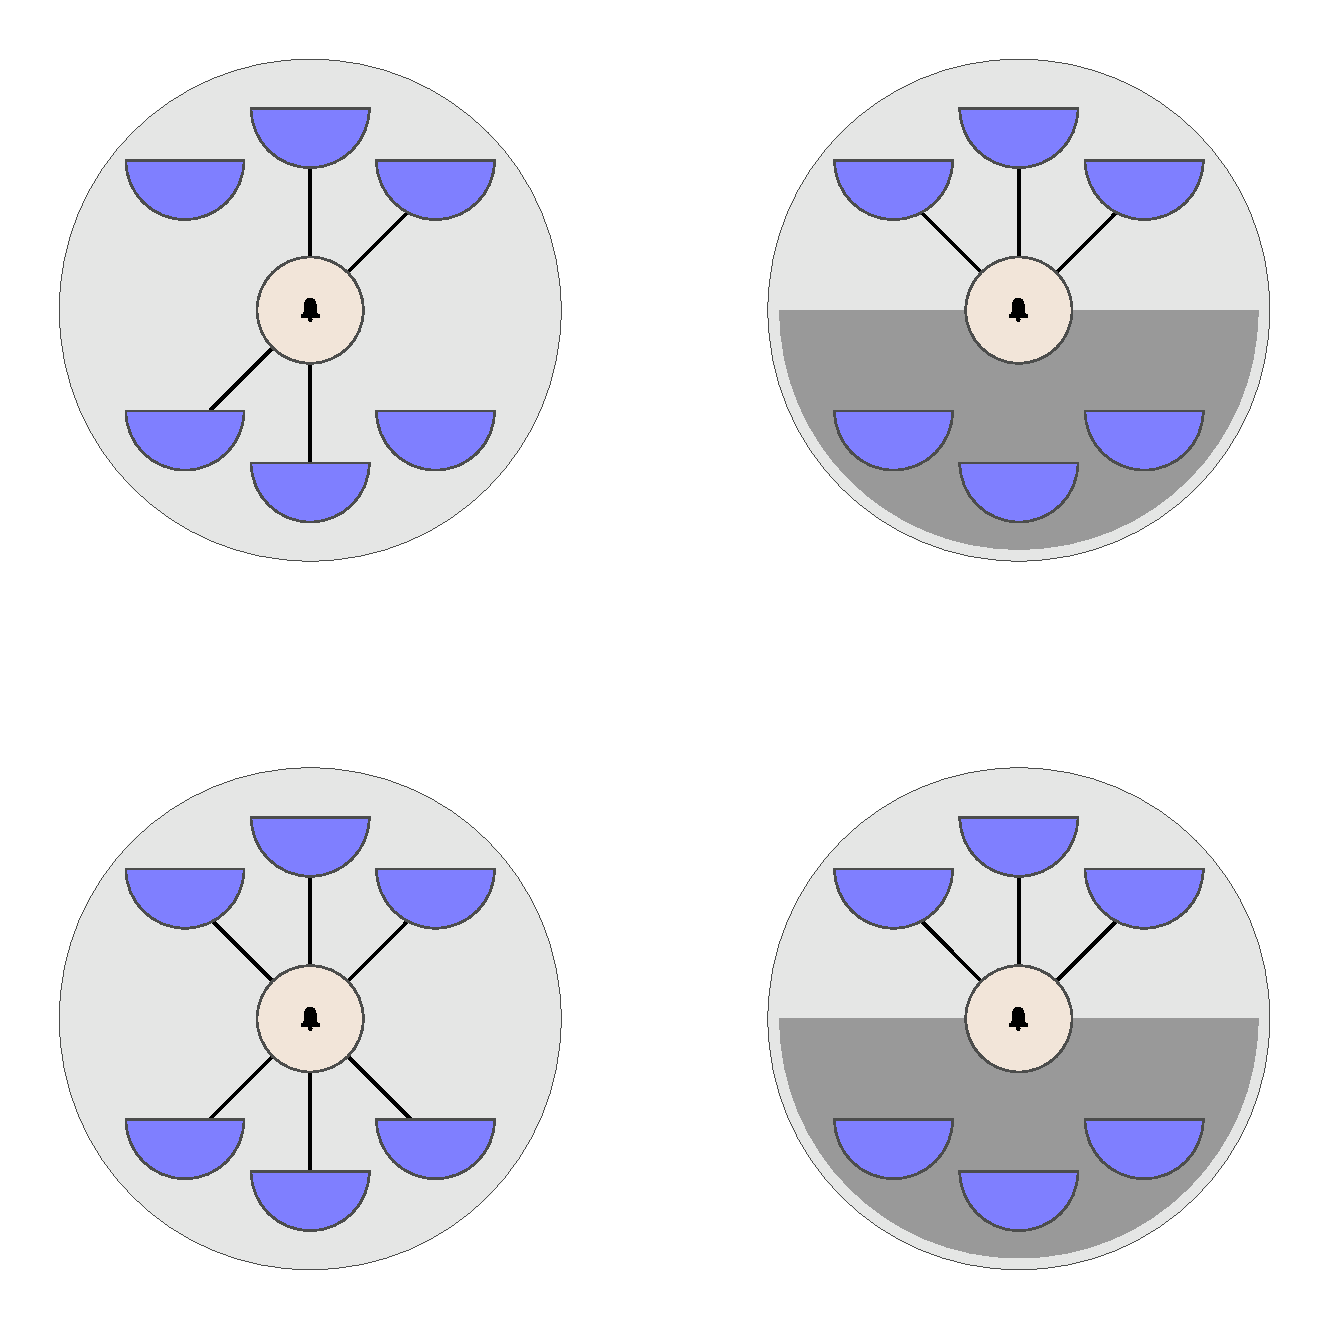
\includegraphics[width=3.5cm]{../pictures/ge_01_4.pdf}}
	    \label{fig:exseqES4}
	}
	\subfloat[][Step 5 (\loc true)]{
		\fbox{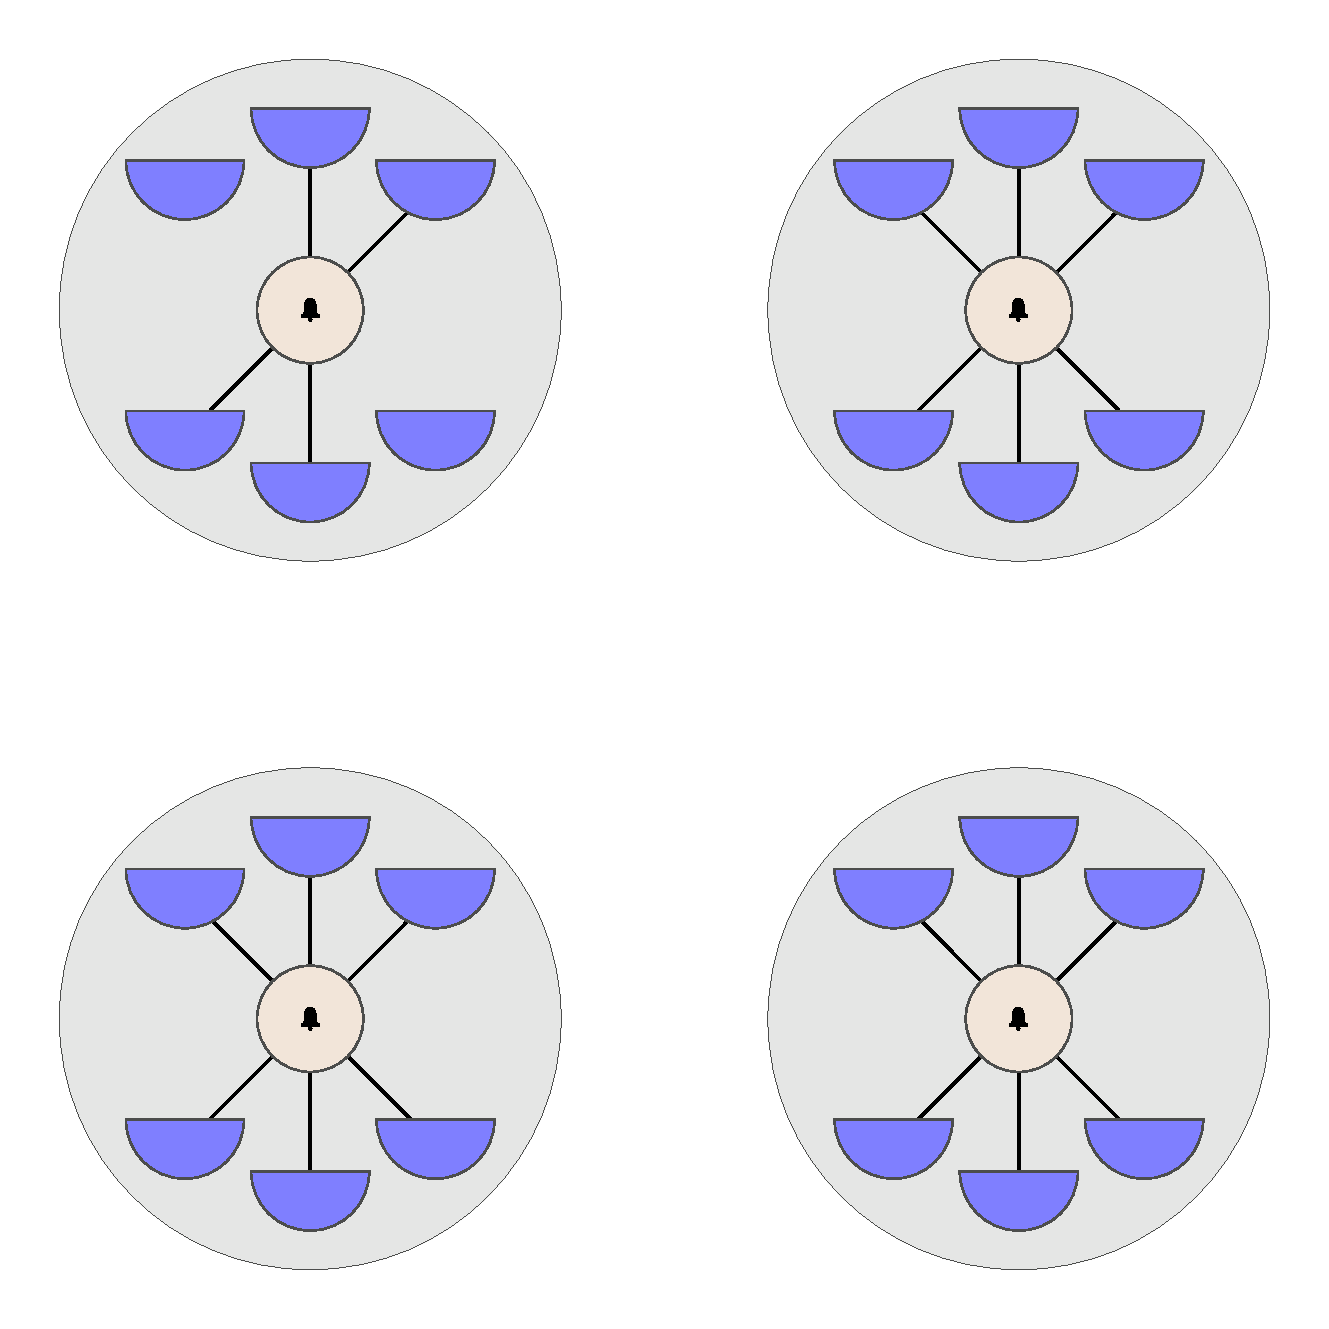
\includegraphics[width=3.5cm]{../pictures/ge_01_5.pdf}}
	    \label{fig:exseqES5}
	}
                \hspace*{3.9cm} 
	\caption[]{Example sequence for \es-sentences.}
	\label{fig:exseqES}
\end{figure}
%
For a sentence like (\ref{ex:es}) we obtain an unambiguous mapping
between truth judgements and readings with the sequence in
\ref{fig:exseqES}.
\begin{exe}
\ex \label{ex:es} \gll \mymark{Genau} eine der Glocken ist mit
  \mymark{einigen} ihrer Halbkreise verbunden.\\ 
  Exactly one of-the bells is with some its semicircles connected.\\
  \trans Exactly one bell is connected to some of its semicircless.
\end{exe}
The critical positions are steps 2, 3 and 5. At step 2 in
Figure~\ref{fig:exseqES2}, a global reading would yield a \emph{false}
judgement. The literal reading can be evaluated at step 3 in
Figure~\ref{fig:exseqES3}, where it would trigger a \emph{false}
judgement. Finally, confirming \ref{fig:exseqES5} by a \emph{true}
response indicates a local reading. Note that global and literal
readings again differ from local readings with respect to their truth
values.


\paragraph{Positional controls.} To make sure that subjects understood
the task, i.e., gave truth-value judgements at the first possible
position in a sequence, we included a set of control conditions. These
also controlled for response biases. For each of the three readings in
the \as- and \es-conditions, we constructed an unambiguous control
sentence as in (\ref{bsp:controls-as}) and (\ref{bsp:controls-es}),
requiring the same judgement at the identical position in the same
sequence used for the respective targets. For instance, example
(\ref{bsp:controls-as-1}) requires a \emph{true}-response analogous to
the \as-sentence in (\ref{ex:as}) under its literal reading at step 3
in Figure~\ref{fig:exseqAS3}, (\ref{bsp:controls-as-2}) corresponds to
the \as-sentence under its global reading and
(\ref{bsp:controls-as-3}) corresponds to its local reading. With
regard to the \es-sentences, controls like (\ref{bsp:controls-es-1})
correspond to the global reading, (\ref{bsp:controls-es-2}) to the
literal and (\ref{bsp:controls-es-3}) to the local reading. If,
independently of sentence meaning, there was any bias to respond in a
certain way at any point in the sequences, such as to preferably
unravel the whole picture, this should affect control sentences to the
same degree as it affects target conditions.

\begin{exe}
  \ex \label{bsp:controls-as}
    \begin{xlist}
\ex \label{bsp:controls-as-1} \gll Alle Briefe sind mit mindestens drei ihrer Dreiecke verbunden.\\
  All letters are with at-least three their triangles connected.\\
  \trans All letters are connected to at least three of their triangles.
\ex \label{bsp:controls-as-2} \gll Mindestens ein Brief ist mit genau f\"unf seiner Dreiecke verbunden.\\
  At-least one letter is with exactly five his triangles connected.\\
  \trans At least one letter is connected with exactly five of its triangles.
\ex \label{bsp:controls-as-3} \gll Jeder Brief ist mit mindestens vier seiner Dreiecke verbunden.\\
  Every letter is with at-least four his triangles connected.\\
  \trans Every letter is connected to at least four of its triangles.
\end{xlist}
\end{exe}

\begin{exe}
\ex \label{bsp:controls-es}
  \begin{xlist}
\ex \label{bsp:controls-es-1} \gll Alle Glocken sind mit weniger als
  vier ihrer Halbkreise verbunden. \\ 
All bells are with fewer than four their semicircles connected.\\
\trans All bells are connected with fewer than four of their semicircles.  
\ex \label{bsp:controls-es-2} \gll Alle Glocken sind mit allen ihren Halbkreisen verbunden.\\
All bells are with all their semicircles connected.\\
\trans All bells are connected to all of their semicircles. 
\ex \label{bsp:controls-es-3} \gll Mindestens drei Glocken sind mit
  allen ihren Halbkreisen verbunden.\\ 
  At-least three bells are with all  their semicircles connected.\\
  \trans At least three bells are connectd with all of their semicircles.
\end{xlist}
\end{exe}

\paragraph{Preference-related controls.} In order to test whether the
order of critical positions for different readings within a sequence
had an influence on responses, we included a second type of control
conditions. Moreover, these controls served as a test whether the
incremental verification task could possibly detect at least ordinal
preference relations among multiple candidate readings. Finally, these
conditions also controlled whether prosodic information can, in
principle, shift answer patterns in the present task. Note that for
our target sentences, the logical entailment relations between
readings always require local readings to be evaluated at the end of a
sequence. It could thus in principle be possible that subjects never
reach this point, because they give truth-value judgements earlier,
thereby ending the trial. In that case it would be unclear if these
decisions had been affected by a general unavailability of local
readings or by the fact that one of the earlier presented readings is
the preferred one. By including globally ambiguous structures with a
known preference over available readings, we thus intended to test
whether participants in our task occasionally choose dispreferred
readings, even if these were available only at a critical position
following the preferred readings.

We therefore included globally ambiguous \emph{late-closure
  sentences} as in (\ref{bsp:target-related}), which have been
repeatedly shown to exhibit interpretive preferences.
\begin{exe}
\ex \gll Der Brief ist mit Kreisen und Vierecken mit Sonnen
  verbunden. \label{bsp:target-related}\\
The letter is with circles and squares with suns connected.\\
The letter is connected with circles and squares with suns.
\begin{xlist}
  \ex \label{bsp:target-related-LC} The letter is connected with squares containing suns, and it is
    also connected with circles. \hfill{(\lc)}
  \ex \label{bsp:target-related-EC} The letter is connected with circles and squares, both of which
    are containing suns.  \hfill{(\ec)} 
\end{xlist}

\end{exe}
In late-closure sentences, a modifier such as a relative clause or a
prepositional phrase (\acro{pp}) can be attached to one of two
preceding hosts. For instance, in (\ref{bsp:target-related}), the
\acro{pp} \emph{with suns} can be attached to the preceding noun
\emph{squares}, resulting in the so-called \emph{late-closure} (\lc)
reading ((\ref{bsp:target-related-LC}). Alternatively, the \acro{pp}
can be attached to the whole conjoined \acro{np} \emph{circles and
  squares}, corresponding to the \emph{early-closure} (\ec) reading
(\ref{bsp:target-related-EC}).  \lc-readings have been observed to be
preferred over \ec-readings for sentences comparable to those in
(\ref{bsp:target-related}) \citep[e.g.][]{Frazier87,Frazier82}.

For each such sentence, two sequences were designed: one in which the
preferred \lc-reading could be judged first (Figure~\ref{fig:exlc}),
%
\begin{figure}[]
	\centering
	\subfloat[][Step 2]{ 
		\fbox{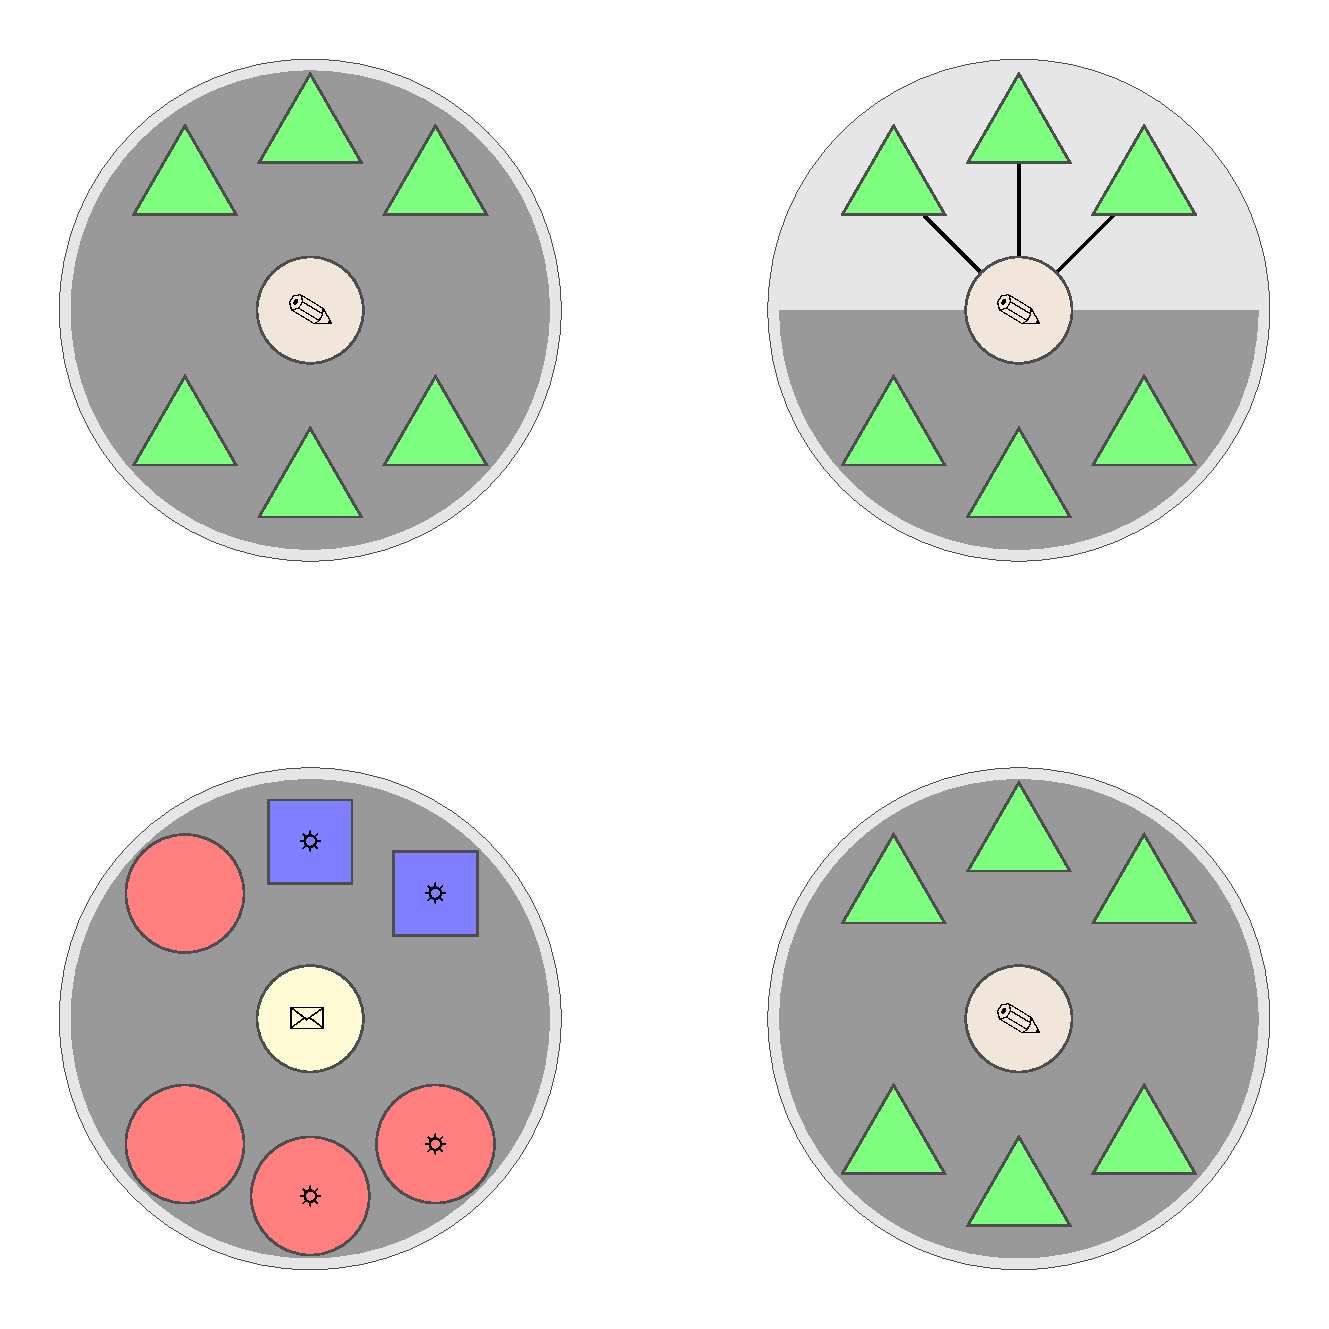
\includegraphics[width=5cm]{../pictures/lc_01_2.pdf}}
	    \label{fig:exlc2}
	}
	\subfloat[][Step 3 (\lc true)]{
		\fbox{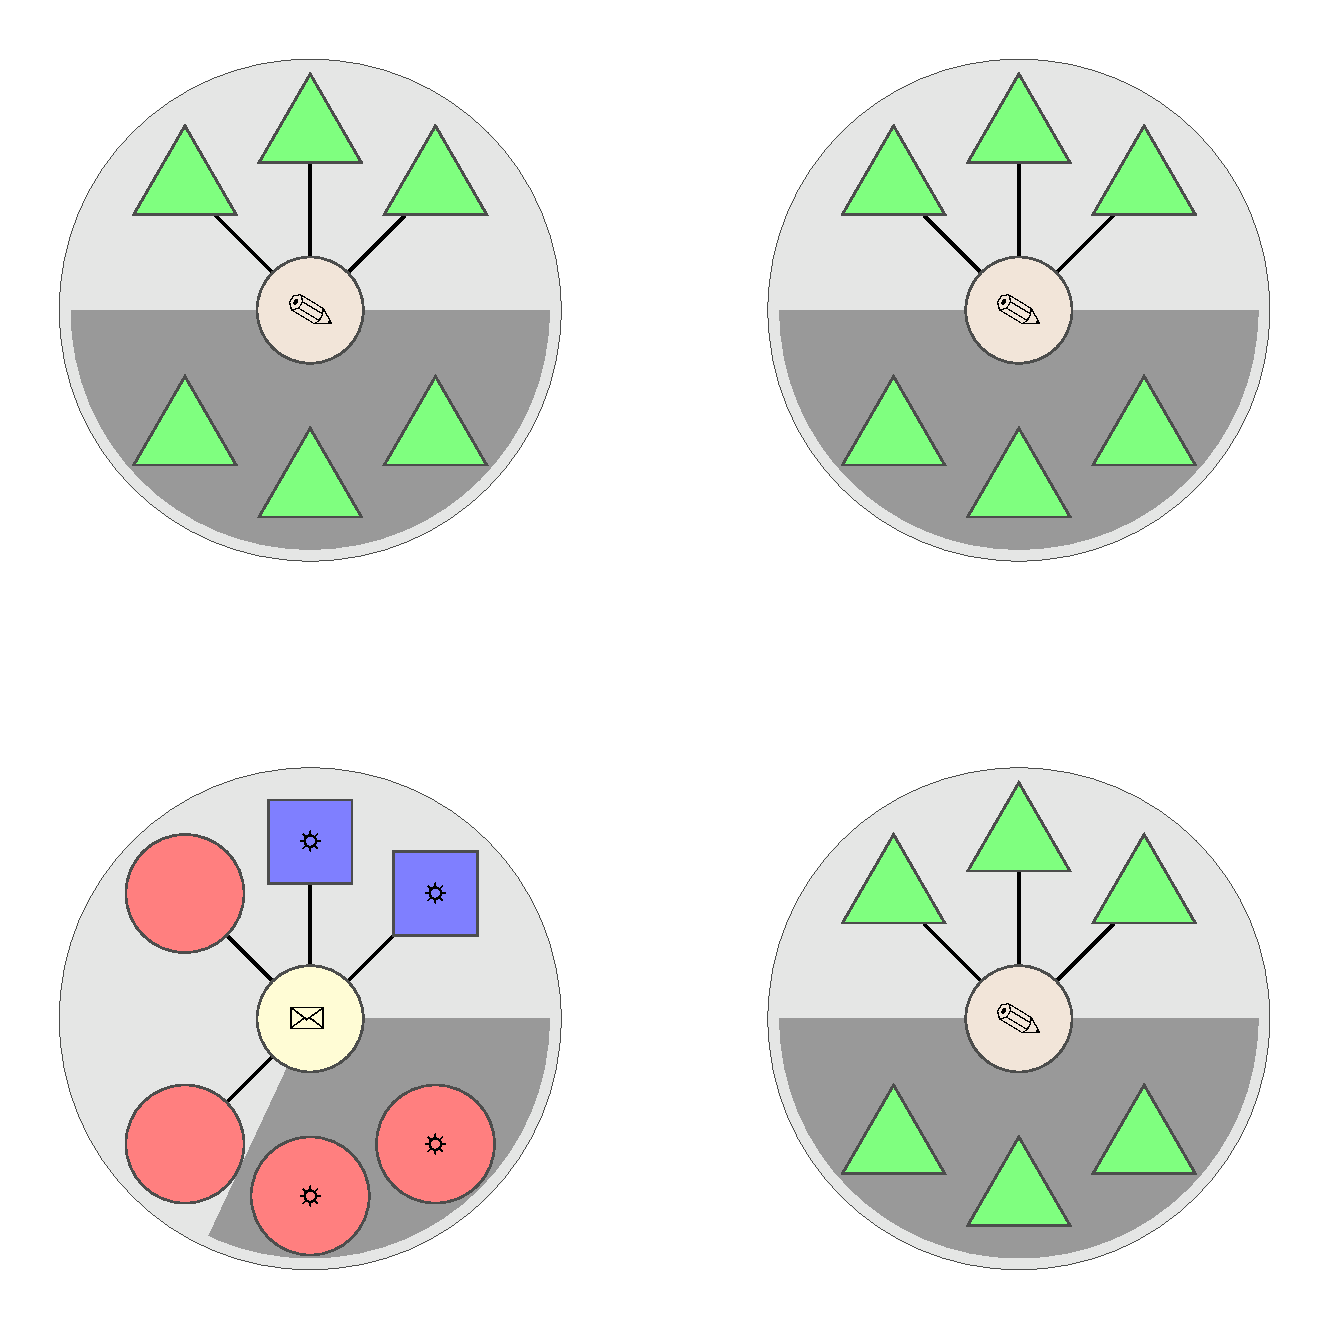
\includegraphics[width=5cm]{../pictures/lc_01_3.pdf}}
	    \label{fig:exlc3}
	}
        \\
	\subfloat[][Step 4]{
		\fbox{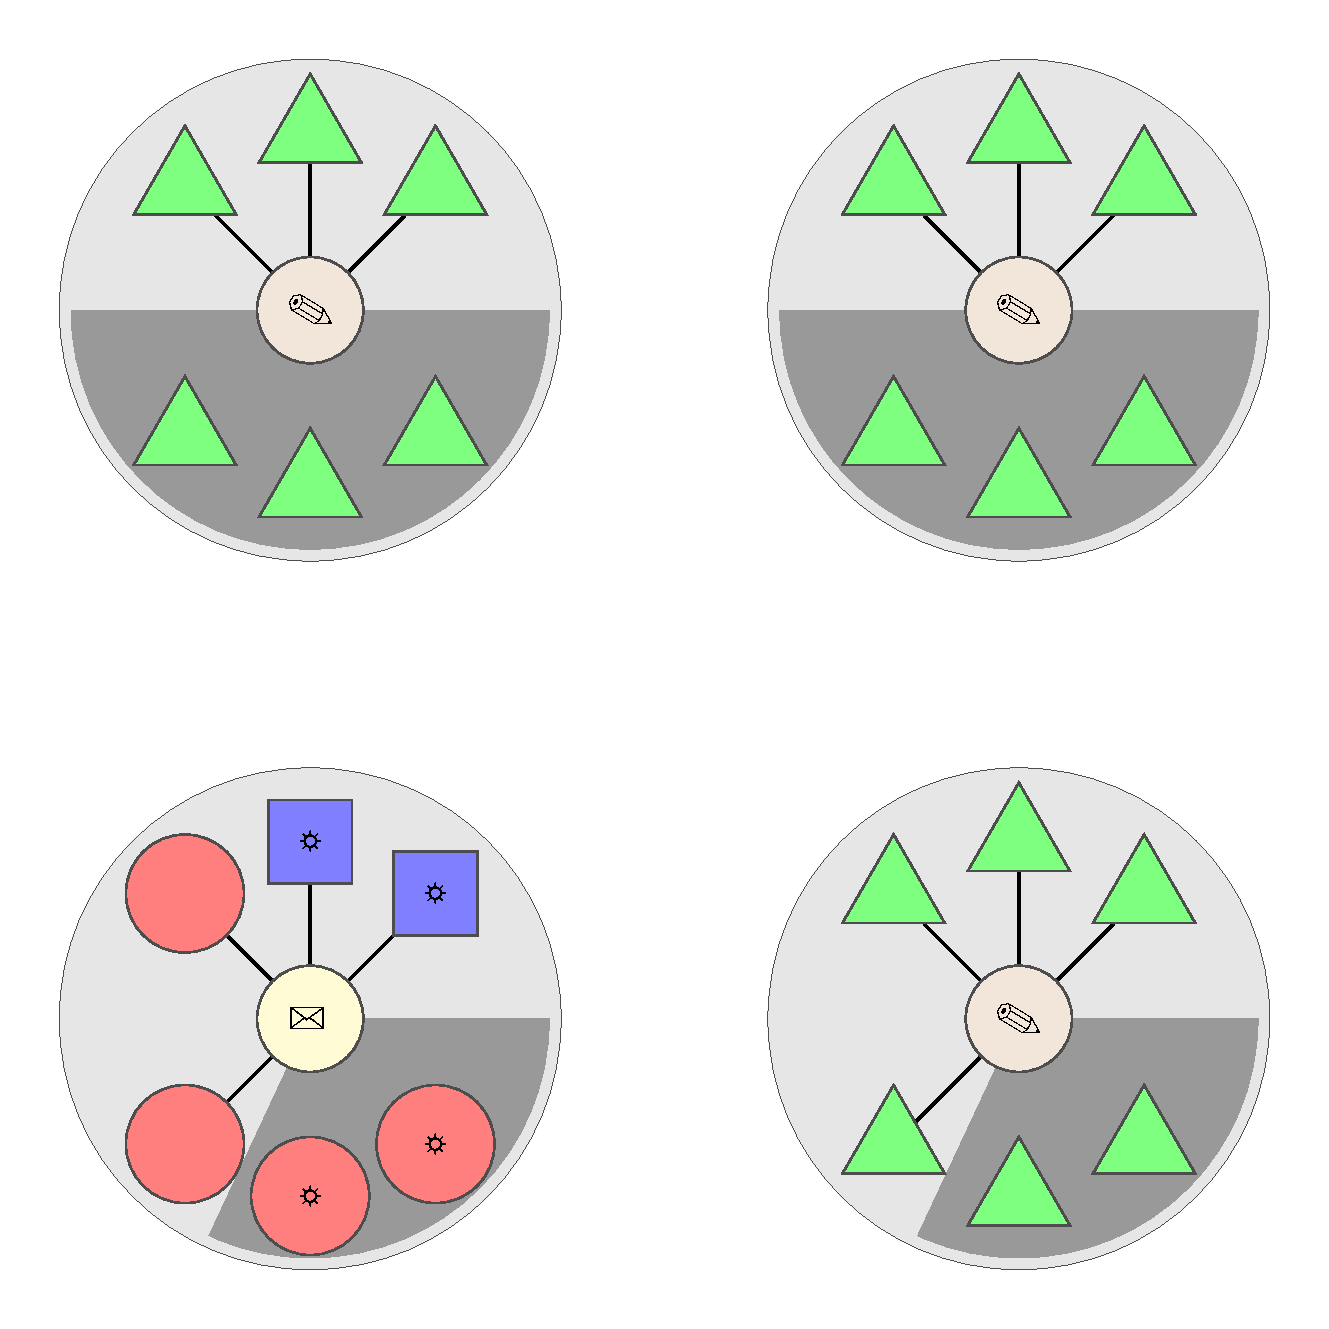
\includegraphics[width=5cm]{../pictures/lc_01_4.pdf}}
	    \label{fig:exlc4}
	}
	\subfloat[][Step 5 (\lc true)]{
		\fbox{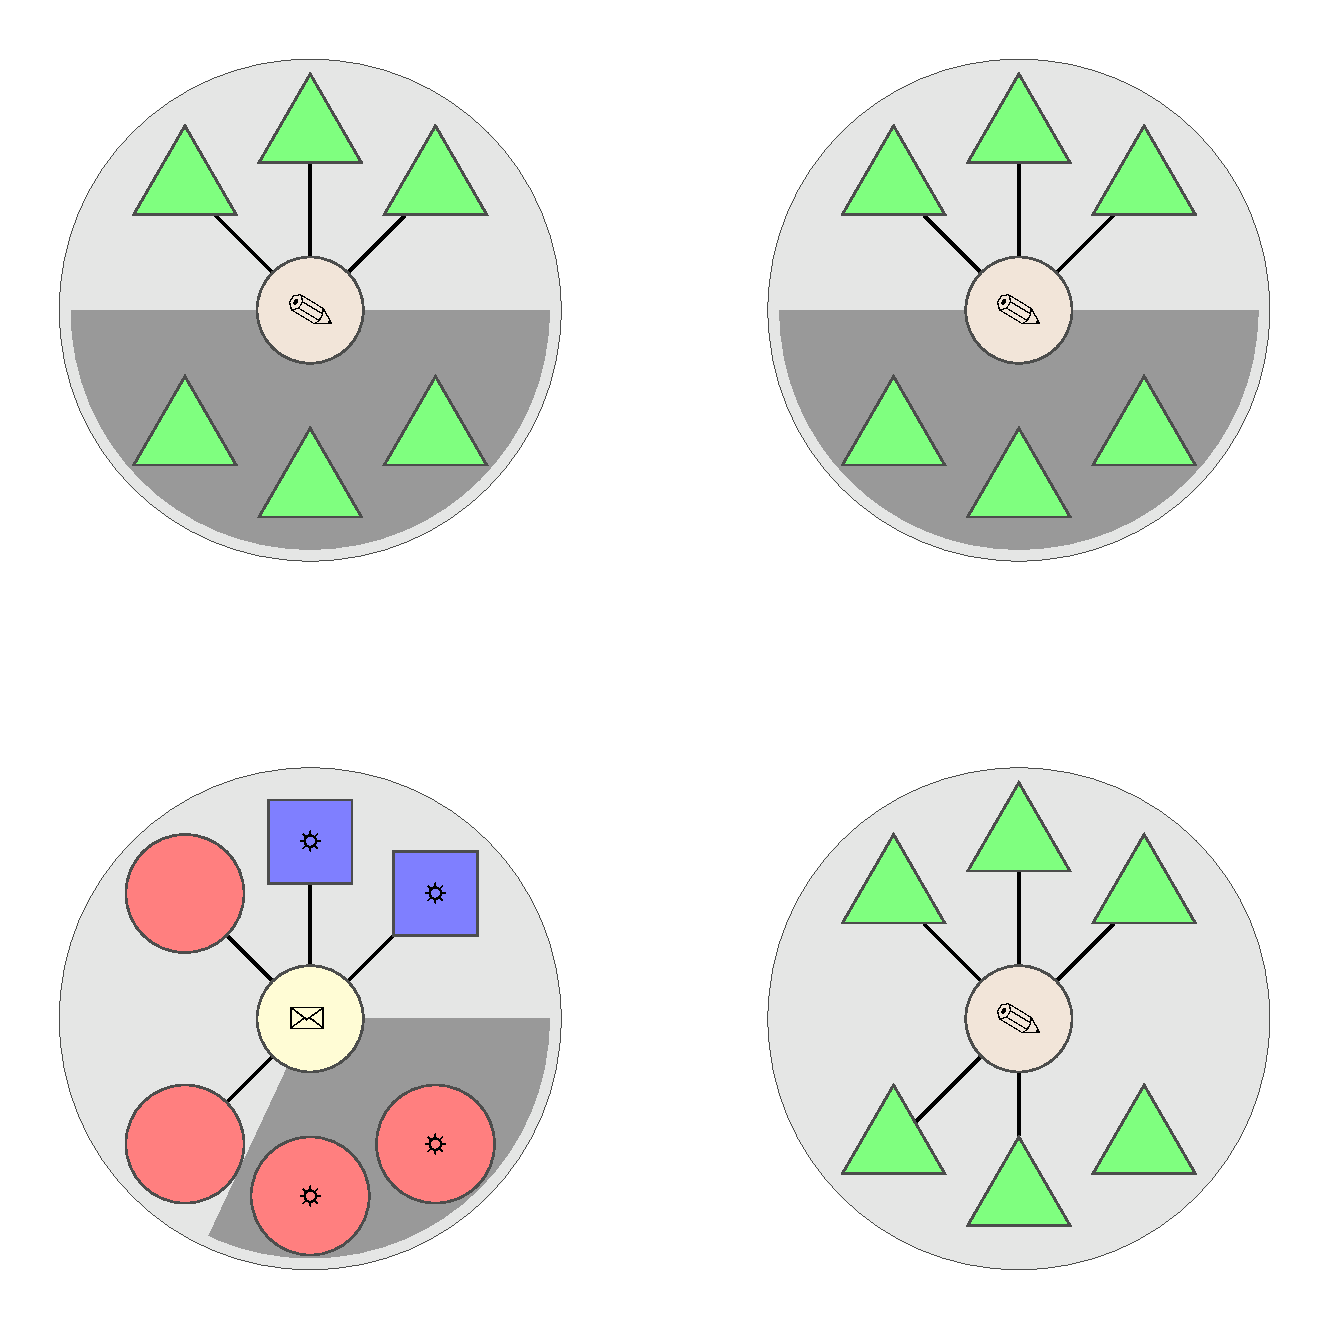
\includegraphics[width=5cm]{../pictures/lc_01_5.pdf}}
	    \label{fig:exlc5}
	}
        \\
	\subfloat[][Step 6 (\ec false)]{
		\fbox{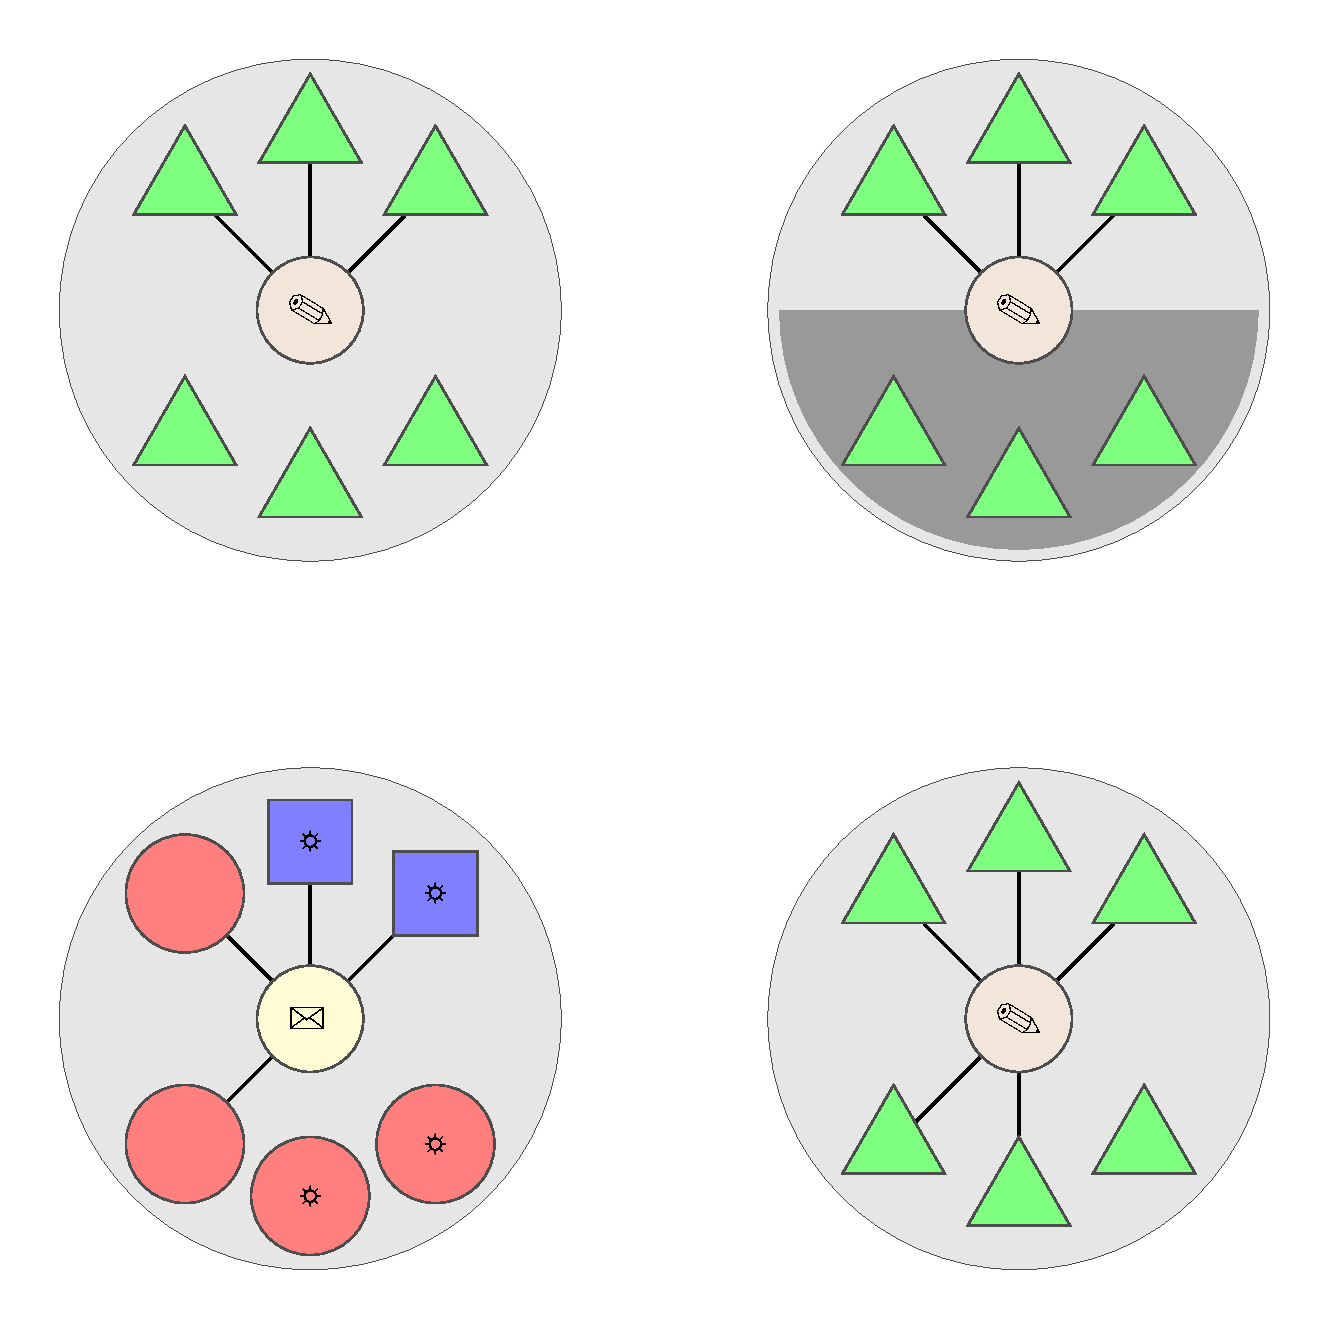
\includegraphics[width=5cm]{../pictures/lc_01_6.pdf}}
	    \label{fig:exlc6}
	}
	\subfloat[][Step 7 (\lc true)]{
		\fbox{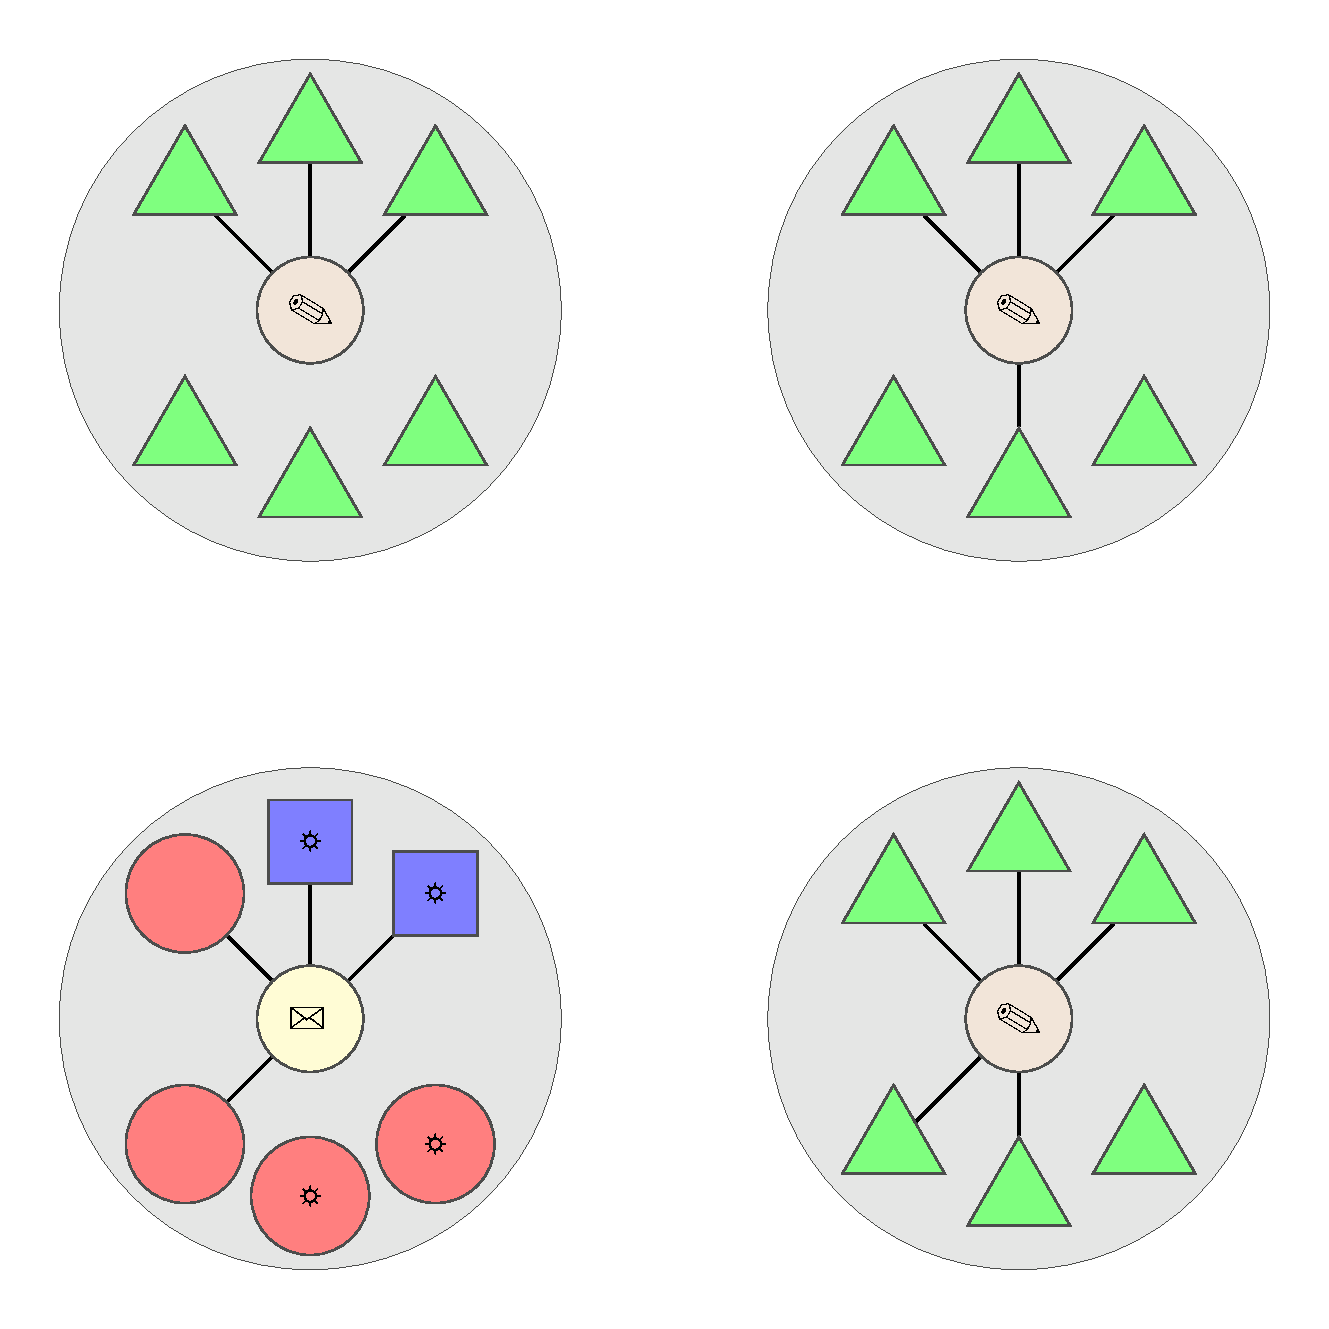
\includegraphics[width=5cm]{../pictures/lc_01_7.pdf}}
	    \label{fig:exlc7}
	}
	\caption[]{Example of an \lc-sequence for sentence
          (\ref{bsp:target-related}) where the \lc-reading
          (\ref{bsp:target-related-LC}) can be judged first. The first
          step where all connections are covered is omitted.}
	\label{fig:exlc}
\end{figure}
%
and another in which the dispreferred \ec-reading could be judged
first (Figure~\ref{fig:exec}).
%
\begin{figure}[]
	\centering
	\subfloat[][Step 2]{ 
		\fbox{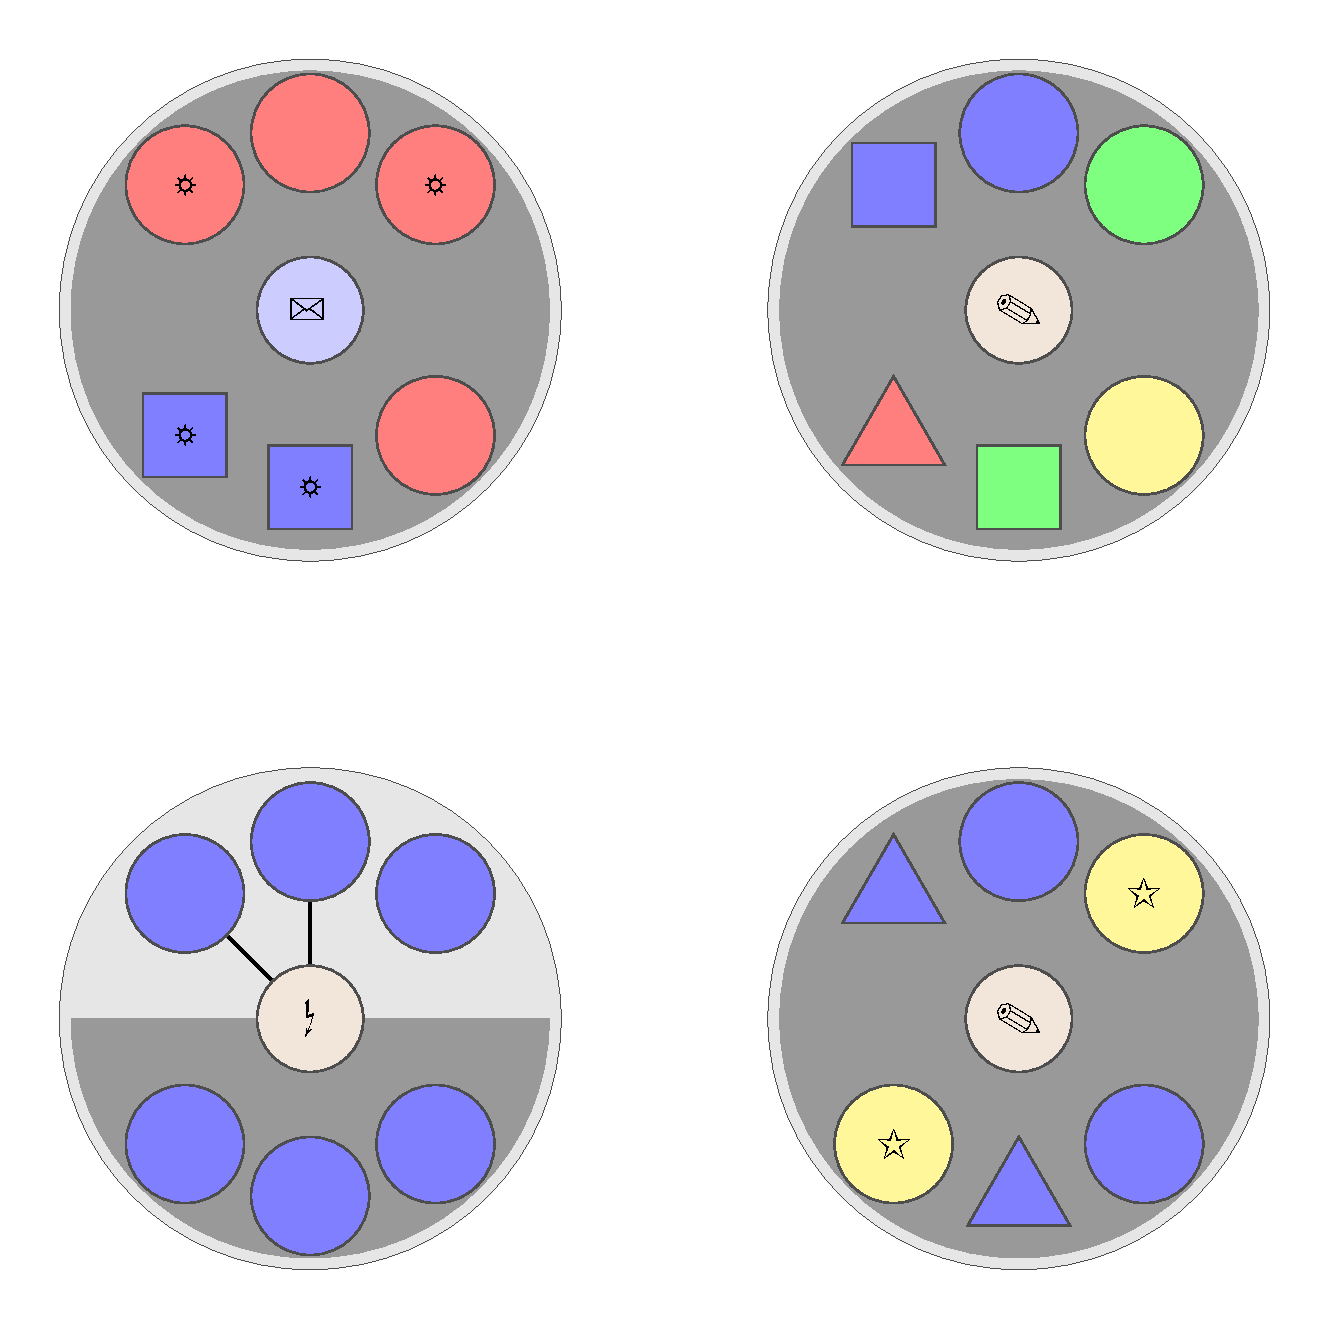
\includegraphics[width=5cm]{../pictures/ec_01_2.pdf}}
	    \label{fig:exec1}
	}
	\subfloat[][Step 3 (\ec false)]{
		\fbox{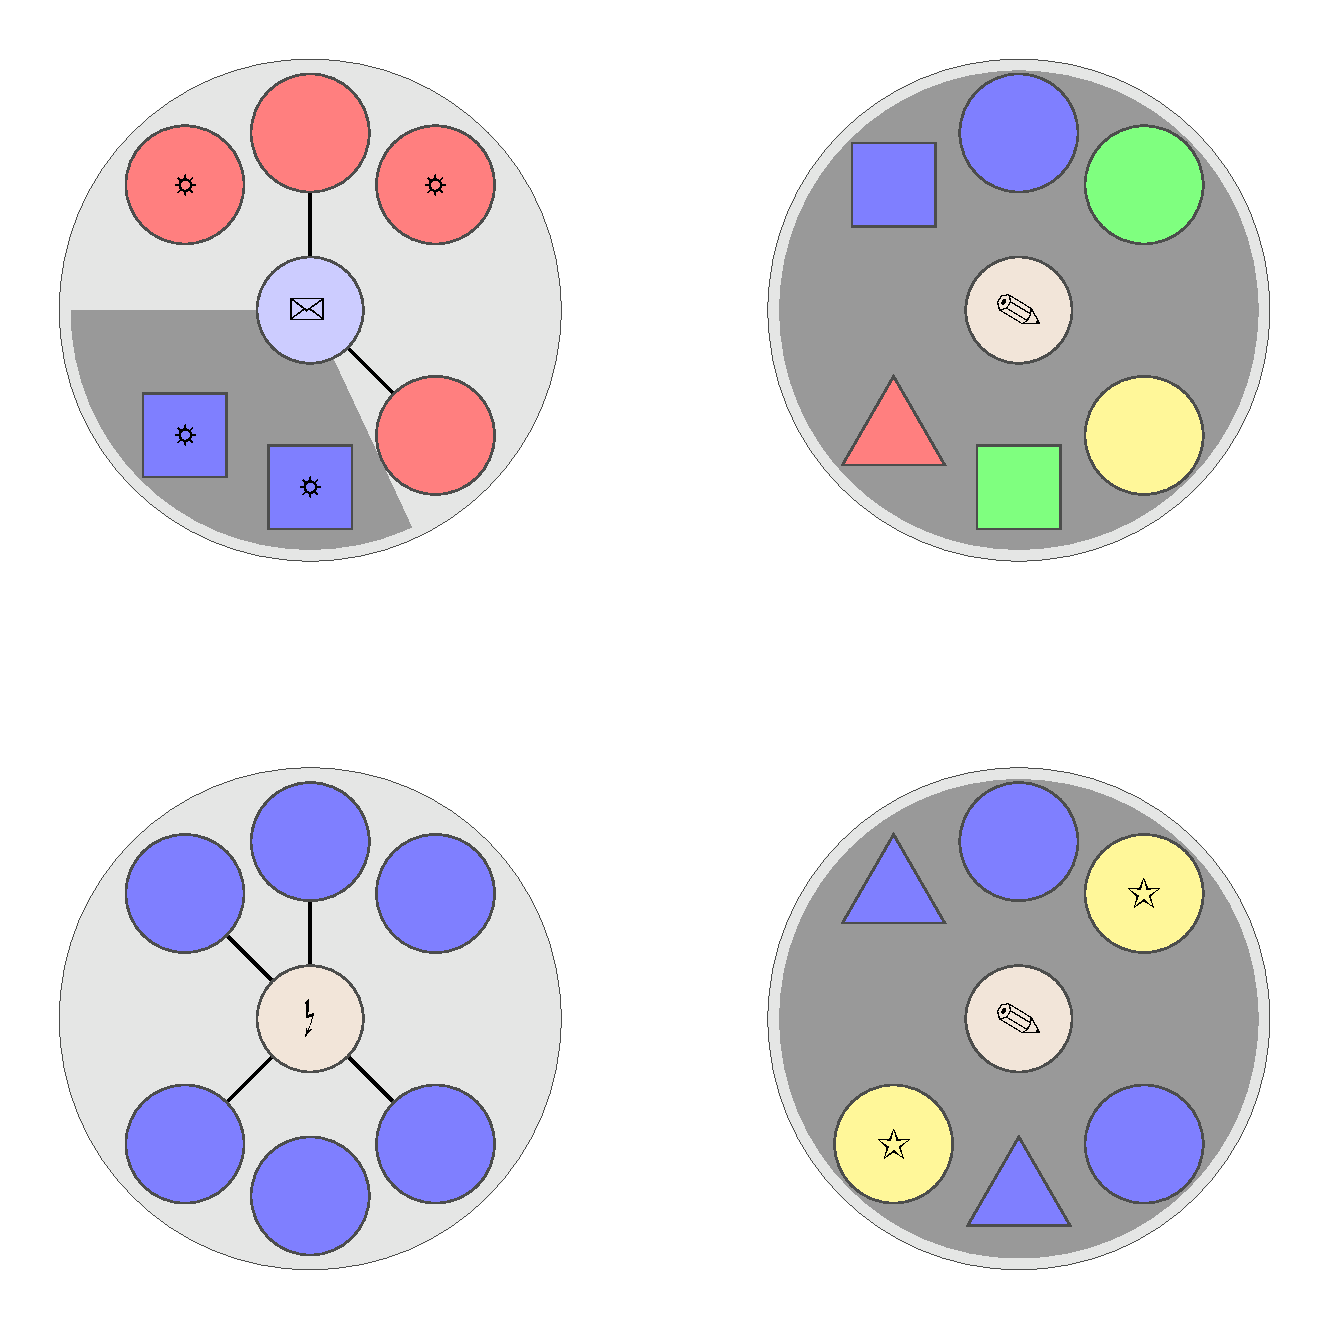
\includegraphics[width=5cm]{../pictures/ec_01_3.pdf}}
	    \label{fig:exec2}
	}
        \\
	\subfloat[][Step 4]{
		\fbox{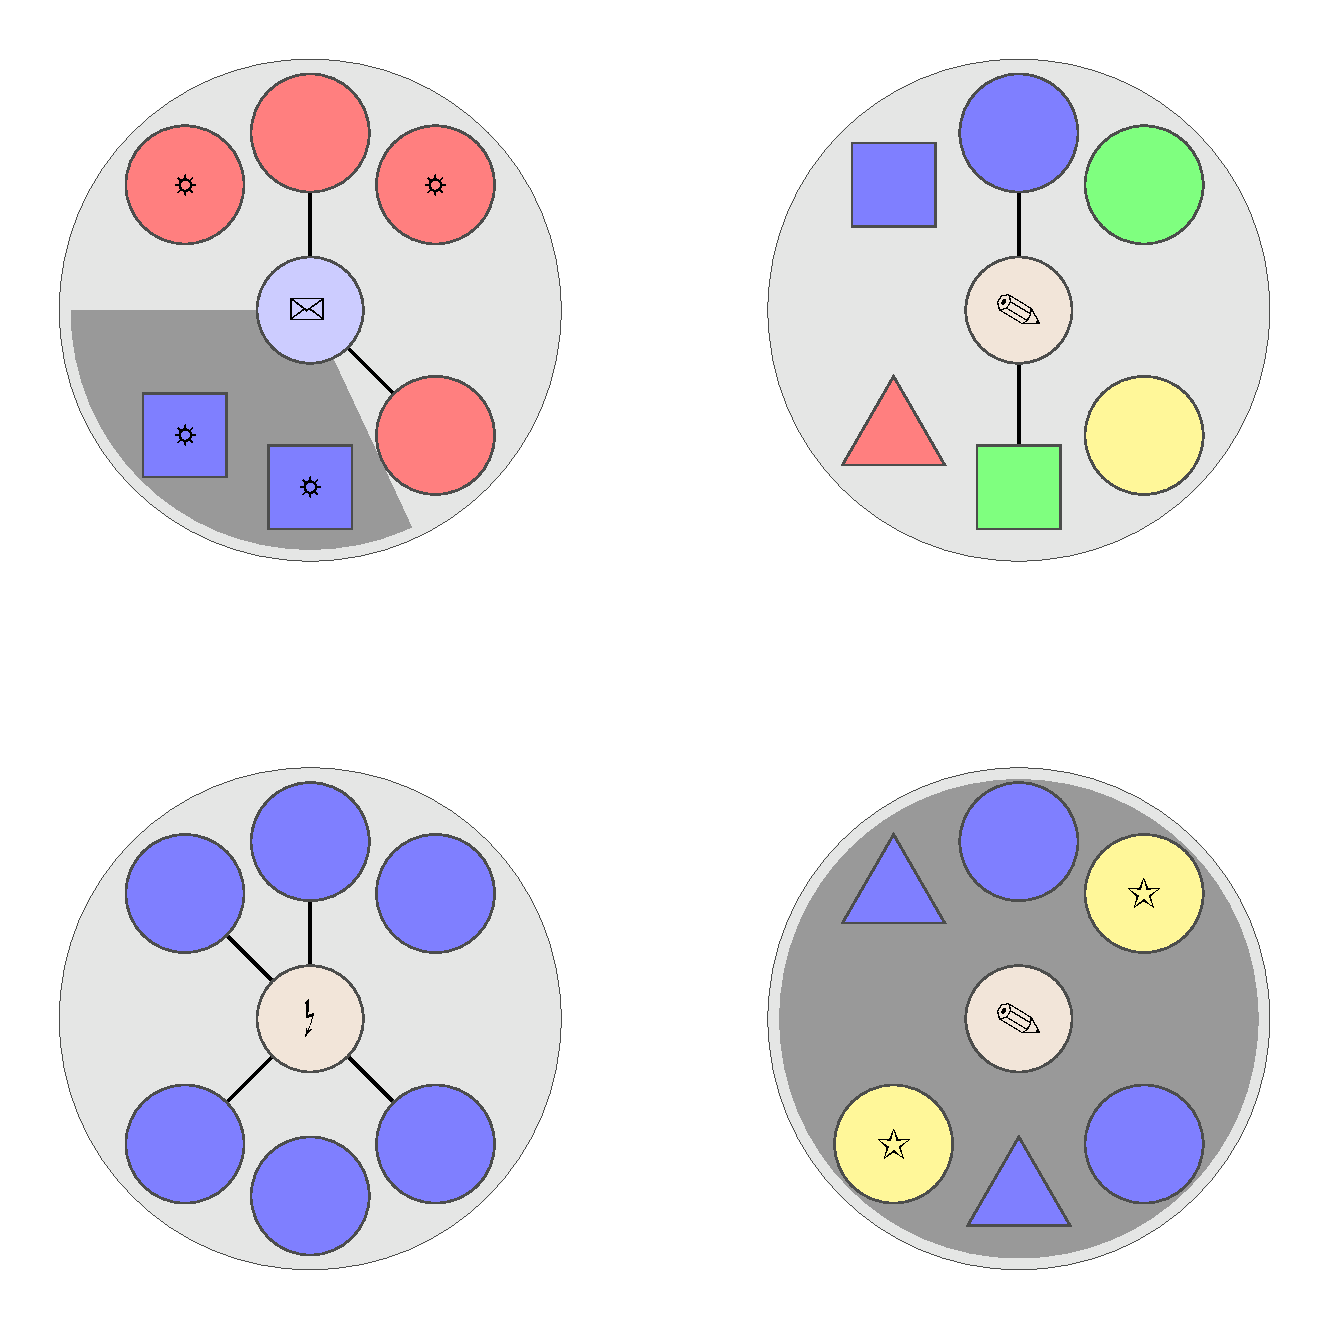
\includegraphics[width=5cm]{../pictures/ec_01_4.pdf}}
	    \label{fig:exec2}
	}
	\subfloat[][Step 5 (\lc true)]{
		\fbox{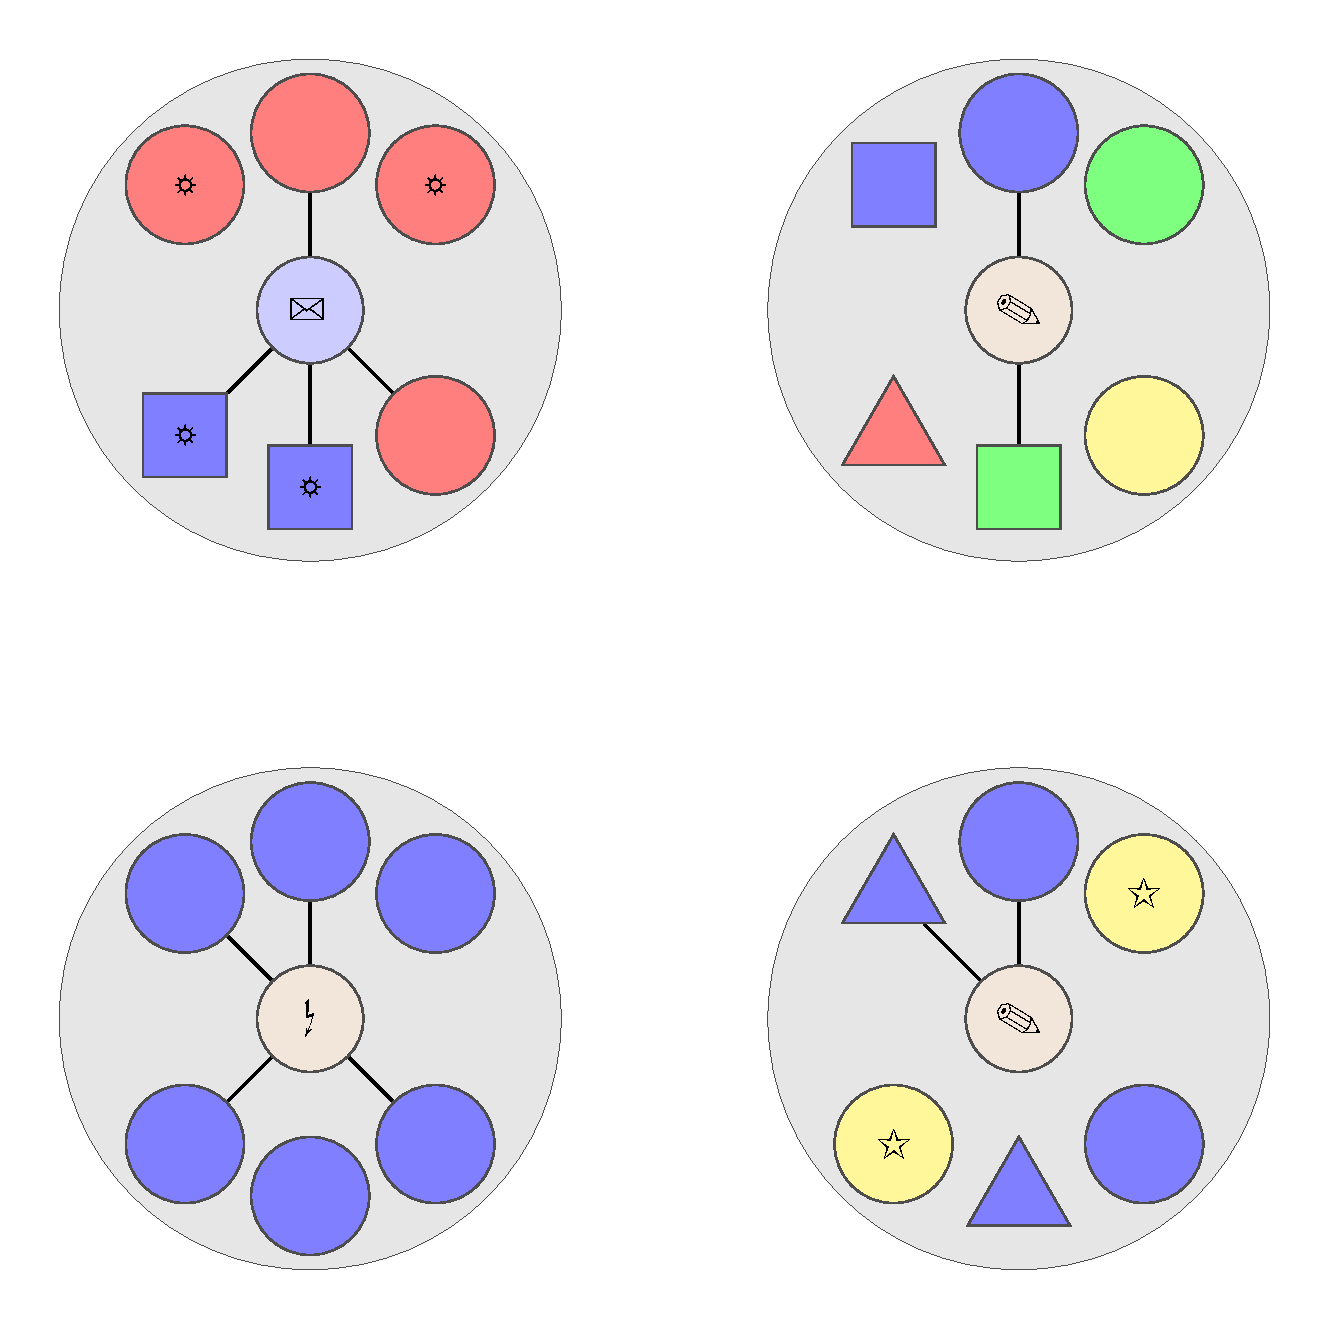
\includegraphics[width=5cm]{../pictures/ec_01_5.pdf}}
	    \label{fig:exec2}
	}
	\caption[]{Example of an \ec-sequence for sentence
          (\ref{bsp:target-related}) where the \ec-reading
          (\ref{bsp:target-related-EC}) can be judged first. The first
          step where all connections are covered is omitted.}
	\label{fig:exec}
\end{figure}
%
We also tested structurally disambiguated versions like
(\ref{bsp:target-related2}), one for each sentence type, on each
sequence type for proper comparison.

\begin{exe}

\ex \gll Der Brief ist mit Kreisen, die Sonnen beinhalten, und Vierecken
  verbunden. \label{bsp:target-related2}\\
The letter is with circles, which suns contain and squares connected.\\
The letter is connected with circles containing suns, and with squares.  

\end{exe}


\paragraph{Testing Effects of prosody.} Whereas contrastive accents
are usually assumed to be realized by a special contour in English
(i.e. L+H*, see \citet{Pierrehumbert90}), the exact phonological
classification of contrast in German is still under debate
\citep[see][]{Uhmann91,Fery93,Grabe98,Toepel06, Sudhoff10}.  Still,
all of these approaches have in common that from an acoustic
perceptive, prosodic prominence of contrastively accented constituents
is realized by

\begin{enumerate}[(i)]
\item a higher F0 maximum or a higher pitch range (difference 
between minimal and maximal F0 values), and
\item a longer duration of the accented element as opposed to its 
non-accented counterpart.
\end{enumerate}

\noindent We therefore recorded sentences by a phonetically trained
female native speaker of German familiar with the concept of
contrastive focus and instructed her to produce contrasts as described
above. Both \as-sentences and \es-sentences were recorded in two
versions each. In the accented version, a contrastive stress was
placed on {\it einige}. The second version had neutral prosody.  If
accentuation is the driving force for local readings, we would expect
a higher proportion of local readings in the former than in the latter
version of the sentences.

Preference-related controls also differed prosodically. Modifier
attachment ambiguities have been shown to be sensitive to differences
in prosodic phrasing. Though there has been discussion as to whether
speakers reliably \textit{produce} disambiguating cues in such
constructions \citep[e.g.][]{Allbritton96,Kraljik05, Snedeker03,
  Schafer00}, overt prosodic boundaries are generally acknowledged to
guide interpretive processes of late-closure sentences in
\textit{comprehension} \citep[e.g.][]{Steinhauer99, Augurzky06}.
Specifically, it has been shown that prosodically separating a
modifier from the directly preceding material supports an \ec-reading,
whereas separating the two potential attachment sites is supportive of
an \lc-reading. Thus, a phrase boundary between {\it squares} and {\it
  with} in (\ref{bsp:target-related}) corresponds to an \ec-reading,
whereas a prosodic phrase boundary following {\it circles} corresponds
to an \lc-reading.

To test whether prosodic information is taken into account in our
task, we presented sentences in both of these prosodic variants. In
addition, in order to test prosody-independent preferences, we also
included a neutral version without any pronounced boundary. Further,
we also presented unambiguous sentences corresponding to the
\ec-reading. As in the case of the \as- and \es-sentences,
the unambiguous counterparts served as a baseline to control for
response biases that are independent of sentence meaning.


\subsection{Procedure}
\label{sec:procedure} 
Each experimental trial proceeded as described above. The sentence was
presented using active PC loudspeakers and the picture materials were
presented on a computer screen. Participants responded using the
keyboard. By pressing one of four buttons they could (i) listen to the
sentence (up to three times), (ii) request additional pictorial
information, (iii) respond "yes, fits" or (iv) "no, does not fit". At
the beginning of an experimental session participants received written
instructions on their task. Then they completed an interactive
training consisting of 15 trials in which they were familiarized with
the task.  After the training the actual experiment
started. Participants were tested individually in a silent room. Each
session was divided into three blocks and participants were told that
they could take breaks between blocks. In total, an experimental
session took about one hour. At the end of the session participants
received 8 euros compensation.


\subsection{Materials}
\label{sec:materials}


\paragraph{Target sentences and positional controls.}

We constructed a set of 15 items for German \as- and \es-sentences,
respectively, analogous to the examples in (\ref{ex:as}) and
(\ref{ex:es}). Sentences were introduced by a subject {\acro{dp}},
including the quantifiers {\it alle diese} ("all of these") or {\it
  genau eine(r) der} ("exactly one of these"), as well as the head
noun which denoted different icons, such as letters or bells. Subjects
were followed by an auxiliary, and a \acro{pp} containing {\it
  einige}, a possessive pronoun, and a noun denoting a geometrical
object, e.g., {\it einigen seiner Dreiecke/Quadrate} ("some of its
triangles/squares"). The possessive pronoun was used in order to fix
relative quantifier scope to surface scope, thus ensuring that {\it
  einige} has embedded status. The last word was the main verb {\it
  verbunden} ("connected").  Each sentence was recorded in a stressed
and an unstressed version of scalar {\it einige}. As described above,
three control sentences were created for each experimental item,
corresponding to the critical positions in the course of uncovering
the accompanying sequences.  The positional controls were recorded
with neutral prosody.  Items were evenly distributed across 5 lists
using a Latin square design.


\paragraph{Preference-related control sentences.}
For controlling preferences, 28 sentences that were ambiguous between
a \lc and an \ec-reading, as well as 28 of their
disambiguated counterparts were constructed as described above. In
these sentences, subject \acros{dp} were always denoting icons and
were followed by an auxiliary. In the ambiguous sentences, the
auxiliary was followed by two {\it mit}-\acros{pp}.  The first of
these \acros{pp} consisted in a coordination of two nouns denoting
geometrical objects, whereas the second \acro{pp} denoted icons. In
contrast to these sentences, the unambiguous sentences contained only
one \acro{pp} with a conjunction the first part of which was modified
by a relative clause.

\paragraph{Acoustic properties.}
% A phonetically trained female native speaker of German was instructed
% to realize two prosodic versions of each target sentence, and three
% versions of the ambiguous preference-related controls. In addition to
% these sentences, the unambiguous preference-related controls, the
% positional controls and a set of unrelated fillers were also
% recorded. For these constructions, the speaker was instructed to
% realize prosodic contours as neutral and natural as possible.

For all target sentences (\as and \es), the determiner \emph{einige} was
produced with a contrastive pitch accent as well as with a neutral
accent. % Contrastive accents in German are realized by an increase in F0 (range)
% as well as by a longer duration (see Section~\ref{sec:design} above). 
A set of 15 
experimental items was recorded for each condition (\as vs.~\es, \emph{accented} 
vs.~\emph{unaccented}), resulting in a total number of 60 target sentences.

In contrast to the accent manipulation, the ambiguous
preference-related controls differed with respect to prosodic
phrasing. Prosodic phrase boundaries in German are realized by a rise
in F0 as well as by a durational increase on the final part of the
constituent preceding the boundary (prefinal lengthening) plus an
optional pause \citep[e.g.][]{Vaissiere83,Fery93}.  Boundaries for
these control sentences were either realized at the position
separating the second \acro{pp} from the preceding material
(\emph{late boundary}, corresponding to an \ec-reading) or directly
preceding the second conjunct in the first \acro{pp} (\emph{early
  boundary}, corresponding to an \lc-reading). As the prosodic
realization of the targets involved the comparison between an accented
and a neutral variant, we also included a third version of the
ambiguous preference-related controls without any pronounced
boundaries. For each prosodic variant, a set of 30 items was read,
yielding 90 preference-related controls.

Altogether a total number of 300 sentences consisting of 60 target
sentences, 90 ambiguous preference-related controls, 30 unambiguous
preference-related controls, 90 positional control sentences and 30
unrelated fillers was recorded. The session was recorded in an
acoustically shielded booth (44.1\,kHz sampling rate, 16 bit amplitude
resolution).

Before entering the judgment task, experimental items and
preference-related fillers were analyzed with respect to their acoustic
properties. As both accented elements as well as prosodic boundaries
were expected to differ with respect to their F0 and/or durational
properties, we calculated durational values as well as difference
values between minimal and maximal F0 for each word. Since targets
slightly differed with respect to the total number of words as well as
with respect to certain lexical properties (i.e., \emph{seinen}
vs.~\emph{ihren}, we considered the following analysis regions:

\begin{exe}
  \ex
    \begin{xlist}
      \ex $|_{\text{R}1}$~Alle  	\ $|_{\text{R}2}$~diese 
      \ $|_{\text{R}3}$~$\acro{np}_1$  
      \ $|_{\text{R}4}$~sind  \ $|_{\text{R}5}$~mit  \
      $|_{\text{R}6}$~einigen  \ $|_{\text{R}7}$~ihrer 
       \ $|_{\text{R}8}$~{$\acro{np}_2$}  \ $|_{\text{R}9}$~verbunden.
    \ex       $|_{\text{R}1}$~Genau einer  	\ $|_{\text{R}2}$~der 
      \ $|_{\text{R}3}$~$\acro{np}_1$  
      \ $|_{\text{R}4}$~ist  \ $|_{\text{R}5}$~mit  \
      $|_{\text{R}6}$~einigen  \ $|_{\text{R}7}$~seiner 
       \ $|_{\text{R}8}$~{$\acro{np}_2$}  \ $|_{\text{R}9}$~verbunden.
    \end{xlist}
    % \begin{tabbing}
    %   $|_{\text{R}1}$ Genau einer \= 	\ $|_{\text{R}2}$ diese \=
    %   \ $|_{\text{R}3}$ \acro{np}$_1$ \= 
    %   \ $|_{\text{R}4}$ sind \= \ $|_{\text{R}5}$ mit \= \
    %   $|_{\text{R}6}$ einigen \= \ $|_{\text{R}7}$ seiner 
    %   \= \ $|_{\text{R}8}$  \acro{np}$_2$ \= \ $|_{\text{R}9}$
    %   verbunden. \kill
    %   $|_{\text{R}1}$ Alle \> 	\ $|_{\text{R}2}$ dieser \>
    %   \ $|_{\text{R}3}$ \acro{np}$_1$ \> 
    %   \ $|_{\text{R}4}$ sind \> \ $|_{\text{R}5}$ mit \> \
    %   $|_{\text{R}6}$ einigen \> \ $|_{\text{R}7}$ ihrer 
    %   \> \ $|_{\text{R}8}$  \acro{np}$_1$ \> \ $|_{\text{R}9}$
    %   verbunden. \\
    %   $|_{\text{R}1}$ Genau einer \> 	\ $|_{\text{R}2}$ der \>
    %   \ $|_{\text{R}3}$ \acro{np}$_1$ \> 
    %   \ $|_{\text{R}4}$ ist \> \ $|_{\text{R}5}$ mit \> \
    %   $|_{\text{R}6}$ einigen \> \ $|_{\text{R}7}$ seiner 
    %   \> \ $|_{\text{R}8}$  \acro{np}$_1$ \> \ $|_{\text{R}9}$ verbunden.
    % \end{tabbing}
\end{exe}

\noindent Note that differences between Regions 1, 2, 4 and 7 can be expected
due to lexical differences between the \as and \es-conditions. As
preference-related fillers did not differ with respect to their lexical
properties, we carried out word-by-word analyses for these
conditions. Durational values included the respective word plus any
following silent interval. We did not include the
disambiguated fillers in these analyses as they involved very
different sentence types (i.e., constructions involving prepositional
phrases vs.~relative clauses).

\begin{exe}
  \ex $|_{\text{R}1}$ \acro{D}  	\ $|_{\text{R}2}$ $\acro{np}_1$
      \ $|_{\text{R}3}$ ist 
      \ $|_{\text{R}4}$ mit  \ $|_{\text{R}5}$ $\acro{np}_2$   \
      $|_{\text{R}6}$ und  \ $|_{\text{R}7}$ $\acro{np}_3$ 
       \ $|_{\text{R}8}$  mit  \ $|_{\text{R}9}$ $\acro{np}_4$ \ $|_{\text{R}10}$~verbunden.
\end{exe}

For the durational analyses, constituents were automatically labeled
by the \emph{Aligner} tool \citep{Rapp98}, and the
obtained values were manually corrected afterwards. For the targets,
two-factorial \acros{anova} with the factors \acro{Quantifier} (\emph{all}
vs.~\emph{exactly one}) and \acro{Prosody} (accented vs.~unaccented) were
carried out. For the preference-related fillers, we carried out
one-factorial \acros{anova} with the factor \acro{Prosody} (early
boundary, late boundary, neutral prosody). F0 values were extracted by
means of special Praat scripts
(\url{http://www.fon.hum.uva.nl/praat/}). For the present analyses,
differences between minimal and maximal F0 values for each region or
word were calculated. Again, two-factorial \acros{anova} were carried
out for statistical comparison of the target sentences, and one-factorial
\acros{anova} were carried out for preference-related controls.


\paragraph{Targets.} 
Differences between maximal and minimal F0 values for each of the
single words in the sentence are depicted in
Figure~\ref{fig:minmax_targets}. As expected, accented
determiners showed a larger F0 range compared to unaccented versions,
an effect which was confirmed by statistical analyses (effects on
the determiner: \acro{Prosody}: \emph{F}=94.8; \emph{p}<.001); 
Interaction of \acro{Quantifier} and \acro{Prosody}: \emph{F}=13.7; 
\emph{p}<.01). The observed interaction indicates that these differences
are even more pronounced in the \as-condition.

\begin{figure}[]
	\centering
	\subfloat[][\as-sentences]{
          \begin{tikzpicture}[scale=0.75]
  \begin{axis}[
    cycle list name = mylist,
    legend pos = north west,
    ymajorgrids,
    ymax = 250,
    y = 0.5,
    x tick label style = {rotate = 50, anchor = east},
    xtick = data,
    xticklabels = {alle,diese,N1,sind,mit,einigen,ihrer,N2,verbunden}
    ]
    \addplot+[line width = 1.3pt] coordinates {
      (0 ,17.6)
      (1 ,27.4)
      (2 ,82.6)
      (3 ,32.6)
      (4 ,62.4)
      (5 ,211.3333333)
      (6 ,57.6)
      (7 ,36.66666667)
      (8 ,47.13333333)};

  \addplot+[line width = 1.3pt] coordinates {
        (0 ,19.6        )
        (1 ,36.46666667 )
        (2 ,115.1333333 )
        (3 ,60.6        )
        (4 ,46          )
        (5 ,69.86666667 )
        (6 ,46.66666667)
        (7 ,71.4)
        (8 ,61.46666667)};

      \legend{accented, neutral}
  \end{axis}
\end{tikzpicture}
		% \fbox{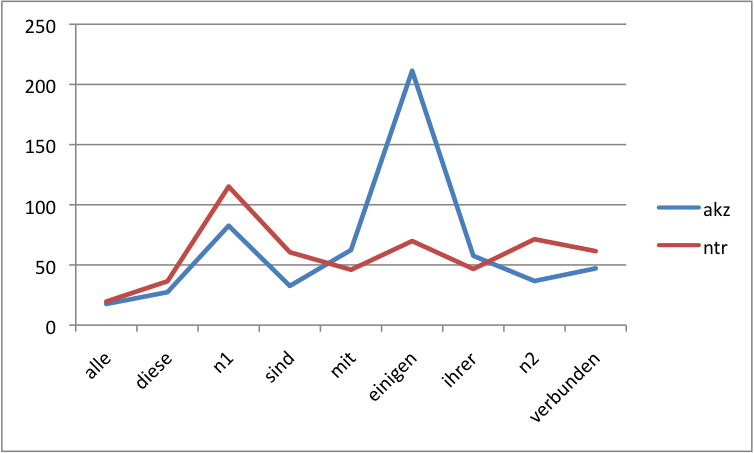
\includegraphics[width=5.5cm]{../pictures/paper/minmax_ae.png}}
	    \label{fig:minmax_ae}
	}
	\subfloat[][\es-sentences]{
\begin{tikzpicture}[scale=0.75]
  \begin{axis}[
    cycle list name = mylist,
    legend pos = north west,
    ymajorgrids,
    ymax = 250,
    y = 0.5,
    x tick label style = {rotate = 50, anchor = east},
    xtick = data,
    xticklabels = {genau,einer,dieser,N1,ist,mit,einigen,seiner,N2,verbunden}
    ]
    \addplot+[line width = 1.3pt] coordinates {
        (     0 , 59.06666667 )
        (     1 , 46.26666667 )
        (     2 , 19          )
        (     3 , 67.6        )
        (     4 , 17.6        )
        (     5 , 39.8        )
        (     6 , 174.9333333 )
        (     7 , 30.46666667 )
        (     8 , 32.46666667 )
        (     9 , 42.33333333 )};

  \addplot+[line width = 1.3pt] coordinates {
        (0 , 30.21428571 )
        (1 , 34.21428571 )
        (2 , 17.07142857 )
        (3 , 93.78571429 )
        (4 , 28.64285714 )
        (5 , 67.64285714 )
        (6, 75.5        )
        (7 , 25.71428571 )
        (8 , 54.85714286 )
        (9 , 55)};

      \legend{accented, neutral}


  \end{axis}
\end{tikzpicture}
		% \fbox{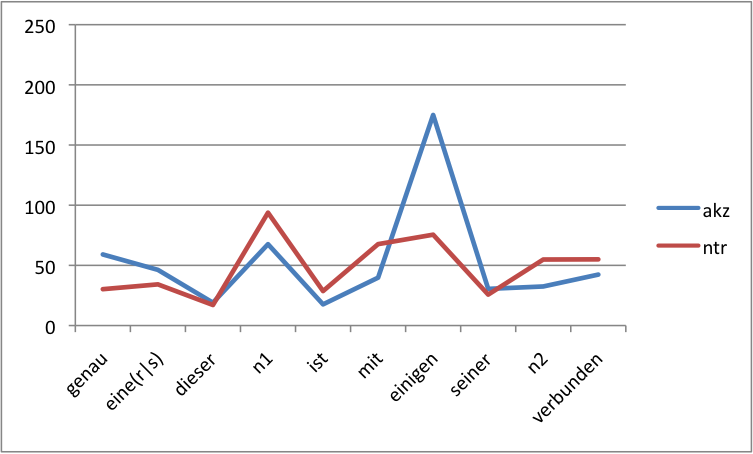
\includegraphics[width=5.5cm]{../pictures/paper/minmax_ge.png}}
	    \label{fig:minmax_ge}
	}
	\caption[]{Differences between minimal and maximal F0 values (in Hz) for 
	the single regions for \as-sentences (a) and \es-sentences (b).}
	\label{fig:minmax_targets}
\end{figure}

\begin{figure}[]
	\centering
	\subfloat[][\as-sentences]{ 
\begin{tikzpicture}[scale=0.75]
  \begin{axis}[
    cycle list name = mylist,
    legend pos = north west,
    ymajorgrids,
    ymax = 800,
    ymin = 0,
    y = 0.125,
    x tick label style = {rotate = 50, anchor = east},
    xtick = data,
    xticklabels = {alle,diese,N1,sind,mit,einigen,ihrer,N2,verbunden}
    ]
    \addplot+[line width = 1.3pt] coordinates {
      (0 ,225.8333333)
      (1 , 245.3333333 )
      (2 , 397         )
      (3 , 172.3333333 )
      (4 , 230.1666667 )
      (5 , 445.8333333 )
      (6, 199.6666667)
      (7, 503)
      (8 ,722 )
    };

  \addplot+[line width = 1.3pt] coordinates {
        (0 , 216.9212    )
        (1 , 234.6666667 )
        (2 , 414.6666667 )
        (3 , 175.5       )
        (4 , 170.5       )
        (5 , 422         )
        (6 , 194.6666667 )
        (7 , 494.6666667 )
        (8 , 748)
};

      \legend{accented, neutral}


  \end{axis}
\end{tikzpicture}
		% \fbox{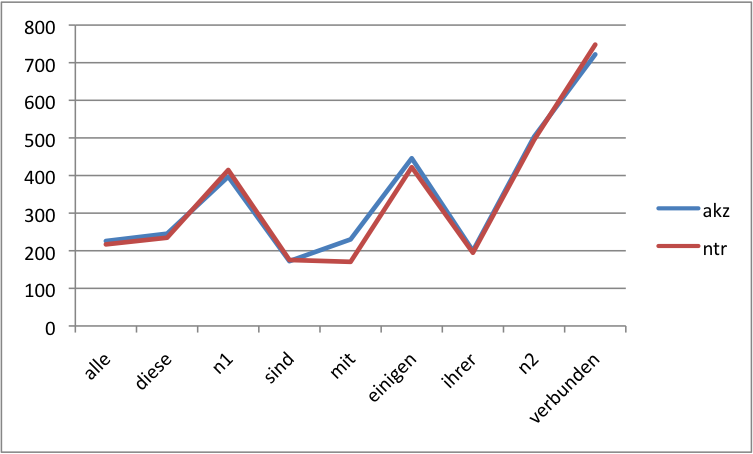
\includegraphics[width=5.5cm]{../pictures/paper/duration_ae.png}}
	    \label{fig:duration_ae}
	}
	\subfloat[][\es-sentences]{
          \begin{tikzpicture}[scale=0.75]
  \begin{axis}[
    cycle list name = mylist,
    legend pos = north west,
    ymajorgrids,
    ymax = 800,
    ymin = 0,
    y = 0.125,
    x tick label style = {rotate = 50, anchor = east},
    xtick = data,
    xticklabels = {genau,einer,dieser,N1,ist,mit,einigen,seiner,N2,verbunden}
    ]
    \addplot+[line width = 1.3pt] coordinates {
(       0 , 307         )
(       1 , 256         )
(       2 , 128.6666667 )
(       3 , 398.6666667 )
(       4 , 164.6666667 )
(       5 , 226.6666667 )
(       6 , 420.6666667 )
(       7 , 235.3333333 )
(       8 , 494.6666667 )
(       9 , 704.6666667 )
    };

  \addplot+[line width = 1.3pt] coordinates {
(0 , 285.8333333 )
(1 , 244.6666667 )
(2 , 128         )
(3 , 400         )
(4 , 152.6666667 )
(5 , 170         )
(6 , 383.3333333 )
(7 , 249.3333333 )
(8 , 494.6666667 )
(9 , 764.6666667 )
};

      \legend{accented, neutral}


  \end{axis}
\end{tikzpicture}
		% \fbox{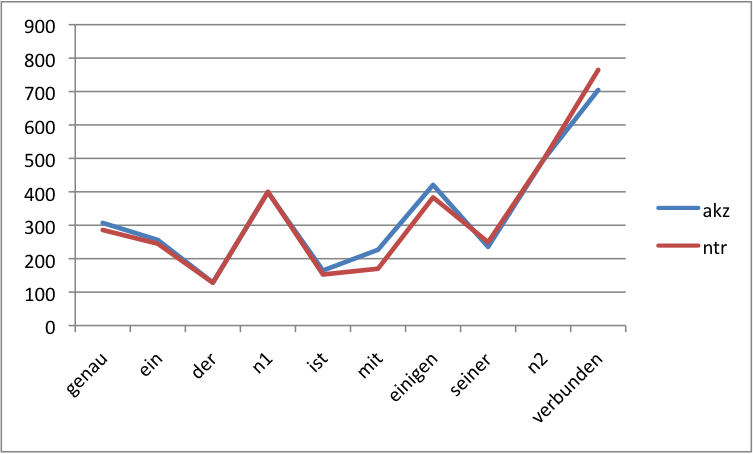
\includegraphics[width=5.5cm]{../pictures/paper/duration_ge.png}}
	    \label{fig:duration_ge}
	}
	\caption[]{Durational values (in ms) for 
	the single regions for \as-sentences (a) and \es-sentences (b).}
	\label{fig:duration_targets}
\end{figure}



Figure~\ref{fig:duration_targets} shows the durational values 
for each of the single regions in the sentence. 
Though descriptively small, the duration of accented determiners 
was significantly increased as opposed to their non-accented counterparts 
(effects on
the determiner: \acro{Quantifier}: \emph{F}=31.4; \emph{p}<.001;
\acro{Prosody}: \emph{F}=23.8; \emph{p}<.001).  



A list of the statistical results of each sentential region is provided in 
Appendix~\ref{sec:audit-sent-mater} (F0 values: Table~\ref{tab:table-B};
durational values: Table~\ref{tab:table-A}).


\paragraph{Preference-related fillers.} 
Differences between maximal and minimal F0 values for each of the
single words in the sentence as well as durational values are depicted in
Figure~\ref{fig:acoustics_fi}. As is
evident, the largest durational and F0 differences were
realized at the boundary regions (i.e. Region 5 and Region
7). 

\begin{figure}[t]
	\centering
	\subfloat[][F0 values]{ 
\begin{tikzpicture}[scale=0.75]
  \begin{axis}[
    cycle list name = mylist,
    legend pos = north west,
    ymajorgrids,
    ymax = 250,
    ymin = 0,
    y = 0.55,
    x tick label style = {rotate = 50, anchor = east},
    xtick = data,
    xticklabels = {D1,N1,ist,mit,N2,und,N3,mit,N4,verbunden}
    ]
    \addplot+[line width = 1.3pt] coordinates {
(       0 ,27.65517241 )
(       1 ,91.20689655 )
(       2 ,32.51724138 )
(       3 ,27.20689655 )
(       4 ,53.72413793 )
(       5 ,19.5862069  )
(       6 ,210.8965517 )
(       7 ,15.48275862 )
(       8 ,66.06896552 )
(       9 ,68.72413793 )
    };

  \addplot+[line width = 1.3pt] coordinates {
(0 ,23.48148148) 
(1 ,63.07407407) 
(2 ,13.7037037 ) 
(3 ,22.7037037 ) 
(4 ,197.0740741) 
(5 ,34.03703704) 
(6 ,95.37037037) 
(7 ,15.22222222) 
(8 ,52.18518519) 
(9 ,123        ) };

  \addplot+[line width = 1.3pt] coordinates {
(0, 31.7        )
(1, 80.2        )
(2, 24.46666667 )
(3, 31.2        )
(4, 135.8333333 )
(5, 54.46666667 )
(6, 86.96666667 )
(7, 16.76666667 )
(8, 51.4        )
(9, 62.53333333 )};

      \legend{\textsc{ec},\textsc{lc},neutral}


  \end{axis}
\end{tikzpicture}
		% \fbox{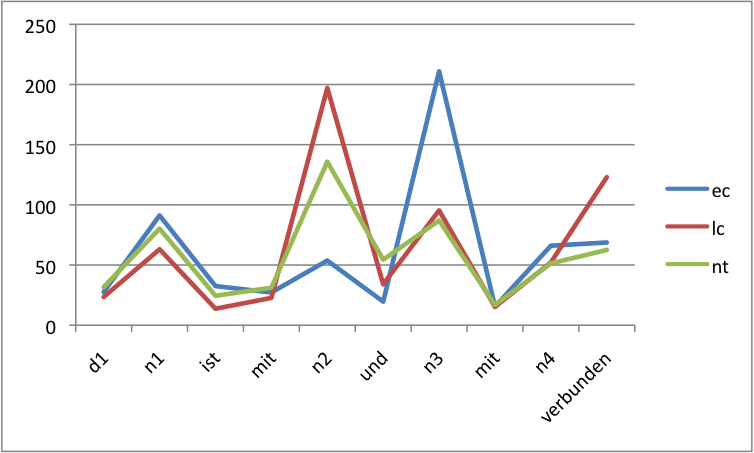
\includegraphics[width=5.5cm]{../pictures/paper/minmax_fi.png}}
	    \label{fig:acoustics_fi}
	}
	\subfloat[][Duration]{
\begin{tikzpicture}[scale=0.75]
  \begin{axis}[
    cycle list name = mylist,
    legend pos = north west,
    ymajorgrids,
    ymax = 1400,
    ymin = 0,
    y = 0.1,
    x tick label style = {rotate = 50, anchor = east},
    xtick = data,
    xticklabels = {D1,N1,ist,mit,N2,und,N3,mit,N4,verbunden}
    ]
    \addplot+[line width = 1.3pt] coordinates {
(0  , 105.75      )
(1  , 332.3333333 )
(2  , 168         )
(3  , 135.3333333 )
(4  , 561.3333333 )
(5  , 143.3333333 )
(6  , 1183.666667 )
(7  , 167         )
(8  , 384.6666667 )
(9  , 691.3333333 )
    };

  \addplot+[line width = 1.3pt] coordinates {
(0  , 100.75      )
(1  , 306.6666667 )
(2  , 167         )
(3  , 139.6666667 )
(4  , 1268.333333 )
(5  , 176.3333333 )
(6  , 535.3333333 )
(7  , 150.3333333 )
(8  , 381         )
(9  , 681.3333333 )
};

  \addplot+[line width = 1.3pt] coordinates {
(0  , 98.08333333 )
(1  , 313.6666667 )
(2  , 169.3333333 )
(3  , 141.3333333 )
(4  , 642.6666667 )
(5  , 150         )
(6  , 557.3333333 )
(7  , 151         )
(8  , 402.6666667 )
(9  , 730)
};

      \legend{\textsc{ec},\textsc{lc},neutral}


  \end{axis}
\end{tikzpicture}
		% \fbox{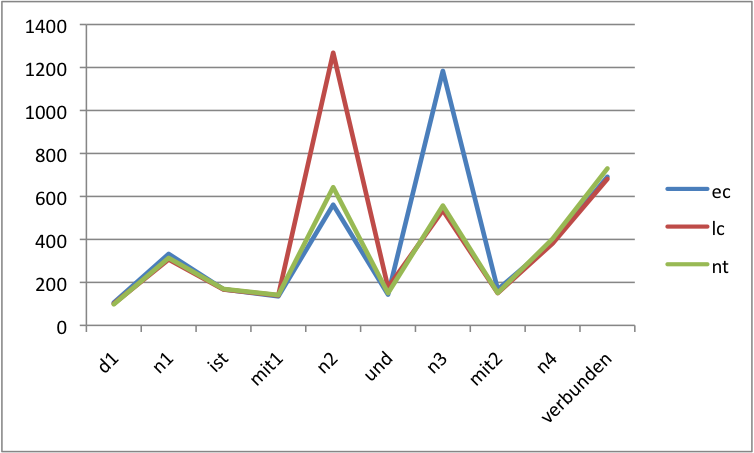
\includegraphics[width=5.5cm]{../pictures/paper/duration_fi.png}}
	    \label{fig:duration_fi}
	}
	\caption[]{Differences between minimal and maximal F0 values (in Hz) (a) as well
	as durational values (in ms)(b) for 
	the single regions  .}
	\label{fig:acoustics_fi}
\end{figure}


Statistical analyses for F0 on Region 5 reveal that all prosodic
realizations (\emph{neutral} vs. (\emph{early boundary}
vs. (\emph{late boundary})) differ significantly from each other
(effect of \acro{Prosody}: \emph{F}=129.3; \emph{p}<.001; all single
comparisons \emph{p}<.001). On Region 7, F0 analyses again show a main
effect of \acro{Prosody}: \emph{F}=132.5; \emph{p}<.001. However, the
comparison between neutral prosody and a \emph{late boundary} did not
reach significance (\emph{p}>.2). Finally, durational analyses on
reveal that all prosodic realizations (\emph{neutral} vs. (\emph{early
  boundary} vs. (\emph{late boundary})) differ significantly from each
other (Region 5: effect of \acro{Prosody}: \emph{F}=819.5;
\emph{p}<.001; all single comparisons \emph{p}<.001; Region 7: effect
of \acro{Prosody}: \emph{F}=1920.3; \emph{p}<.001; all single
comparisons \emph{p}<.001.)

A list of the statistical results of each sentential region is
provided in Appendix~\ref{sec:audit-sent-mater} (F0 values:
Table~\ref{tab:table-D}; durational values: Table~\ref{tab:table-C})

In sum, our speaker reliably
produced (i) differences in accent realization for the target
sentences and (ii) the expected boundary realizations for the
preference-related controls. Whereas accented elements clearly
differed from their unaccented counterpart by showing an increase in
duration and F0 range, prosodic boundaries for our preference-related
fillers were realized by pre-final lengthening (i.e., an increase in F0
and duration at the position preceding the boundary).


\paragraph{Pictures.}
The visual sequences accompanying each sentence consisted of pictures
like in Figures~\ref{fig:exseqAS}--\ref{fig:exlc}. In each picture,
four alternative sub-scenarios were presented, in which an icon was
surrounded by six geometrical shapes. Depending on the sentence
material, shapes and icons differed across sentence types and
conditions. For example, in our target conditions, 4 identical icons
were surrounded by geometrical shapes that were all of the same type,
whereas various icons and surrounding elements were used in each
sequence of the preference-related control structures (see
Section~\ref{sec:design} for more detailed exposition). Pictures for
unrelated fillers had critical positions at random uncovering stages,
including cases where no uncovering was needed for a truth-value
judgement.

\paragraph{Lists.}
Experimental items and preference-related fillers were evenly
distributed across lists. For the \as- and \es-sentences together with
their respective controls, five lists were used employing a Latin
square design. Picture sentence-pairs for the preference-related
controls were spread across eight lists. Each target list was combined
with each list from the preference-related controls, thus yielding to
a total of forty lists. The thirty unrelated filler items were
included in each of these resulting lists.


\subsection{Participants}
\label{sec:participants} 

Forty native speakers of German took part in our study, none of which
had any prior exposure to logic or formal semantics. We excluded two
participants due to insufficient performance on controls ($\le 60\%$
correct answers).


\subsection{Results}
\label{sec:results}

In the following, we will report the results for targets and
preference-related controls separately. After providing the
descriptive results, we present statistical analyses using log-linear
models. We complement these with a Bayesian analysis that is sensitive
to the sequential nature of the incremental verification task and
probes specifically into the preference relations between candidate
readings.

\paragraph{Target conditions and positional controls.}
Performance on positional controls was overwhelmingly correct (90\%
correct responses on average with a variance of 0.012) indicating that
participants understood the task and were able to give correct
truth-value judgments at the adequate point in a sequence. In
general, they were not affected by inessential features of the picture
materials or general response biases.

% \begin{figure}[t] 
% \centering

% \includegraphics[width=0.9\textwidth]{positional_answers_critical.pdf}


% \caption{Answers for the \as- and \es-sequences. Bars show the total
%   number of \emph{yes} (up) and \emph{no} judgments (down) collected
%   at each step during a sequence. E.g., we recorded a total of 103
%   \emph{yes} judgments at the third position in the \as-sequence with
%   neutral intonation, which corresponds to 103 answers that were
%   classified as \emph{literal} answers. Notice that the \as-condition
%   had seven steps, the \es-condition only five.}
% \label{fig:JudgmentsK2}
% \end{figure}
%

\begin{table}
  \centering
  \begin{tabular}{lcccccccc@{\hskip 0.6cm}cccc}
    && \multicolumn{7}{c}{truth value at step}
    & \multicolumn{4}{c}{classification}
    \\ \cmidrule(l){3-9} \cmidrule(r){10-13}
    condition &
    & 1
    & 2
    & 3
    & 4
    & 5
    & 6
    & 7
    & \lit
    & \loc
    & \glb
    & err \\ \midrule
    \as-ntr 
    & T & 1 & 1 & \textbf{103} & 2 & \textbf{0} & 0 & 2 
    & 103 & 3 & 0 & 8 \\
    & F & 0 & 0 & 0 & 0 & 2 & 0 & \textbf{3} \\ 
    \addlinespace[0.25cm]
    \as-acc
    & T & 0 & 1 & \textbf{99} & 2 & \textbf{2} & 0 & 1 
    & 99 & 8 & 5 & 5 \\
    & F & 0 & 0 & 1 & 0 & 0 & 0 & \textbf{8} \\
    \addlinespace[0.25cm]
    \es-ntr
    & T & 0 & 11 & 3 & 1 & \textbf{14} & - & - 
    & 78 & 14 & 0 & 22 \\
    & F & 0 & \textbf{0} & \textbf{78} & 5 & 2 & - & - \\
    \addlinespace[0.25cm]
    \es-acc
    & T & 0 & 10 & 3 & 0 & \textbf{16} & - & - 
    & 78 & 16 & 0 & 20 \\
    & F & 0 & \textbf{0} & \textbf{78} & 5 & 2 & - & -
  \end{tabular}
  \caption{Observed truth-value judgments in critical conditions. The
    left-hand part of the table shows the number of \emph{true} and
    \emph{false} responses obtained at each step in the sequence. The
    right-hand part shows the count for our imposed classification
    scheme. The answer counts indicative of relevant readings are
    given in bold-face on the left-hand side.}
  \label{tab:count_data_CC}
\end{table}


%
% \begin{table}[h]
% \centering

% \begin{tabular}{lccccc}
%   condition & position & \multicolumn{4}{c}{response type} \\ \cmidrule(r){3-6}
%   && \emph{literal} & \emph{local} & \emph{global} & \emph{error} \\
%   \midrule \addlinespace[0.15cm]
%   \textbf{\as neutral} 
%   & Pos 1 & 35 &  0 & 0 & 3 \\
%   & Pos 2 & 35 &  1 & 0 & 2 \\
%   & Pos 3 & 33 &  2 & 0 & 3 \\ \addlinespace[0.15cm]
%   & \textbf{Total} & \textbf{103} &  \textbf{3} & \textbf{0} &
%   \textbf{8} \\
%   \addlinespace[0.25cm]
%   \textbf{\as accented} 
%   & Pos 1 & 33 &  2 & 1 & 2 \\
%   & Pos 2 & 33 &  3 & 1 & 1 \\
%   & Pos 3 & 33 &  3 & 0 & 2 \\ \addlinespace[0.15cm]
%   & \textbf{Total} & \textbf{99} &  \textbf{8} & \textbf{2} &
%   \textbf{5} \\
%   \addlinespace[0.25cm]
%   \textbf{\es neutral} 
%   & Pos 1 & 26 &  5 & 0 & 7 \\
%   & Pos 2 & 26 &  3 & 0 & 9 \\
%   & Pos 3 & 26 &  6 & 0 & 6 \\ \addlinespace[0.15cm]
%   & \textbf{Total} & \textbf{78} &  \textbf{14} & \textbf{0} &
%   \textbf{22} \\
%   \addlinespace[0.25cm]
%   \textbf{\es accented} 
%   & Pos 1 & 26 &  6 & 0 & 6 \\
%   & Pos 2 & 24 &  5 & 0 & 9 \\
%   & Pos 3 & 28 &  5 & 0 & 5 \\ \addlinespace[0.15cm]
%   & \textbf{Total} & \textbf{78} &  \textbf{16} & \textbf{0} &
%   \textbf{20}
% \end{tabular}

% \caption{Contingency table of classified responses for the critical
%   conditions. The factor position encodes whether participants saw the
%   condition in question for the first, second or third time during the
%   whole experiment.}
% \label{tab:CC-ContingencyTable}
% \end{table}
%

Judgements obtained for the four target conditions are listed in
Table~\ref{tab:count_data_CC}. We coded these answers as {\it
  literal}, {\it global} or {\it local} if they were as expected under
one of these readings and as {\it error} if not. The majority of
answers are indicative of a literal reading (90.35\% / 86.84\% in
neutral / accented \as-conditions, and 68.42\% in both neutral /
accented \es-conditions). Only two answers across all critical
conditions fall into the category indicative of global
readings. Judgements indicative of local readings, on the other hand,
are more frequent (2.63\% / 7.02\% for neutral / accented
\as-conditions, and 12.28\% / 14.04\% for neutral / accented
\es-conditions).

The number of responses that fell out of our classification scheme
differs substantially between \as- and \es-conditions. There are
7.02\% / 4.39\% unclassifiable judgements in the neutral / accented
\as-conditions, but 19.30\% / 17.54\% in the neutral / accented
\es-conditions. A look at the right-hand side of
Table~\ref{tab:count_data_CC} reveals that there is some systematicity
in 'error' answers. Most answers that we classified as 'errors' are
plausibly explained as a few random errors, a handful of mistakes
resulting from confusing buttons for \emph{true} and \emph{false} and
a few 'spill-over errors' where participants gave responses one
position too late. There is one notable exception, though. A
substantial number of \emph{true} responses where given at the second
position of \es-sequences (9.65\% / 8.77\%) which is shown in
Figure~\ref{fig:exseqES2}. Although this position in the sequence is
the critical position to reveal a global reading, the latter would be
indicated by a \emph{false} response. It appears that subjects read
\es-sentences as if the non-monotonic quantifier \emph{exactly one}
was a monotonic \emph{at least one}, without pragmatic enrichment of
\emph{some}.\fn{If \emph{some} is pragmatically strengthened under the
  scope of \emph{at least one}, we would expect \emph{true} judgements
  at position 3. Although exactly 3 \emph{true} answers occurred there
  for each neutral and accented \es-conditions, the main point to
  notice is that this misreading of the non-monotonic quantifier does
  not explain \emph{true} judgements at position 5. These are
  therefore still indicative of local readings.} 16 out of the total
21 answers in this category come from 5 subjects, while the remaining
5 were single answers by 5 different subjects.
% subjects 1, 9, 12, 21, 84
This suggests that at least for some subjects non-monotonic
quantifiers were problematic. (We will come back to this point later.)

We fitted generalized linear models to the count data in
Table~\ref{tab:count_data_CC}, using factors \textsc{Condition} with
levels \as and \es, \textsc{Accent} with levels \emph{neutral} and
\emph{accented}, and \textsc{Position} with levels 1 through 3 (coding
whether it was the first, second or third time that a participant saw
a critical condition during the experiment) to predict the dependent
factor \textsc{Reading} with levels \emph{literal}, \emph{local}, and
\emph{other}. The latter lumps \emph{global} and \emph{error}
responses together, because otherwise we would not have enough cell
counts to apply log-linear regression. We determined the ``best''
predictor of the data by a gradient search over hierarchical models in
terms of AICs, starting from the saturated model. The best model takes
main factors \textsc{Response} and \textsc{Condition} into account, as
well as the interaction term \textsc{Response:Condition} ($\chi^2 =
17.19$, $df=42$, $p = 0.99$, $AIC = 158.01$ (compared to $AIC=208.25$
of the saturated model)). Crucially, factors \textsc{Position} and
\textsc{Accent} are spurious in the best model. This suggests that
response patterns only depend on the type of the sentence, but that
there were no learning or fatigation effects and that accentuation did
not influence answer patterns significantly (at this level of
abstraction).

\begin{table}
  \centering
  \begin{tabular}{lllll}
    coefficient & estimate & std.~error & $z$-value & $\Pr(>|z|)$ \\
    \midrule
    \textsc{Intercept} & 0.916  &  0.258 &  3.49  & < 0.001 \\
    \textsc{Reading}.\emph{literal} & 2.600 &   0.268 & 9.716 & < 0.001 \\
    \textsc{Reading}.\emph{local} & -0.310  &  0.397 & -0.781 &
    0.435 \\
    \textsc{Condition}.\es & 1.030 &  0.301 & 3.423 &  < 0.001 \\
    \textsc{Reading}.\emph{literal}:\textsc{Condition}.\es & -1.288 &
    0.319 & -4.036 &  < 0.001 \\
    \textsc{Reading}.\emph{local}:\textsc{Condition}.\es & -0.026 &
    0.463 &  -0.0579 &  0.955
  \end{tabular}
  \caption{Coefficients of the ``best'' log-linear model for the count
    data in Table~\ref{tab:count_data_CC}.}
  \label{tab:Coefficients-CC}
\end{table}

Inspection of the coefficients of the ``best'' model in
Table~\ref{tab:Coefficients-CC} suggests that the distinction between
levels \emph{local} and \emph{other} in factor \textsc{Reading} might
not be necessary: factor levels \emph{local} do not cause a
significant shift in counts, given reference level \emph{false}. In
order to test whether there is support for the postulation of local
readings, we therefore compared the previous ``best'' predictor to a
model that only differs from the former in that it subsumes the level
\emph{local} of factor \textsc{Reading} under level \emph{other} as
well \citep[e.g.][Chapter~15]{Crawley2007:The-R-Book}. Model
comparison reveals that there is no significant improvement in
explanatory power ($Pr(|\chi|) = 0.2689$) of the more complex model
that includes the level \emph{local} (residual df=30, residual
deviance = 10.497) over the simpler model without this level (residual
df=32, residual deviance = 13.124, AIC=157.268).

This latter analysis suggests that our data does not provide strong
evidence for the maintenance of belief in local readings in our
setting. But we need to be careful. The regression analysis tells us
that the number of errors and the number of local readings were
similar in all conditions. But the distribution of answers in
Figure~\ref{fig:JudgmentsK2} shows that small error counts occur at
many different steps, whereas we do see a concentrated rise in answers
at the critical position for local readings. Also, so far we have not
taken into account the sequential structure of our task. It might be
that local readings are infrequent because subjects tend to exit early
in the sequence, rather than late. Or it might be that our count for
local answers is exaggerated by a bias to answer later in the
sequence. This is why we need preference-related controls and a more
fine-grained analysis eventually.

\paragraph{Preference-related controls.} Positional answers for our
preference-related control conditions are shown in
Table~\ref{tab:count_data_TF}.\fn{We removed 19 data points for the
  \ec-conditions because of a coding mistake that presented subjects
  with incongruent sentence-picture pairs. Including these and
  classifying them as \emph{errors} does not change the qualitative
  results of the reported analyses.} Judgments were coded as \ec or as
\lc if they were as expected under one of these readings, and as
\emph{error} if they were not. As expected, most answers classify as
\lc-readings, fewer as \ec-readings. Moreover, intonation does seem to
have the expected effect as well: as compared to neutral intonation,
\lc-cueing intonation increases the count for \lc-readings, while
\ec-cueing increases the count for \ec-readings. If we compare the
number of \lc- or \ec-readings for each intonation type across
sequences, we see that there are always more answers indicative of the
relevant readings when that reading can be judged later in the
sequence. This suggests a general tendency to answer later in the
sequence, rather than at the earliest possible step.

\begin{table}
  \centering
  \begin{tabular}{lcccccccc@{\hskip 0.6cm}ccc}
    && \multicolumn{7}{c}{truth value at step}
    & \multicolumn{3}{c}{classification}
    \\ \cmidrule(l){3-9} \cmidrule(r){10-12}
    condition &
    & 1
    & 2
    & 3
    & 4
    & 5
    & 6
    & 7
    & \lc
    & \ec
    & err \\ \midrule
    \lc-ntr 
    & T & 0 & 0 & \textbf{87} & 1 & 0 & 9 & 0 
    & 87 & 32 & 13 \\
    & F & 0 & 0 & 3 & 0 & 0 & \textbf{32} & 0 \\
    \addlinespace[0.25cm]
    \lc-\lc-cue
    & T & 0 & 0 & \textbf{108} & 1 & 1 & 7 & 0 
    & 108 & 16 & 10 \\
    & F & 0 & 0 & 1 & 0 & 0 & \textbf{16} & 0 \\
    \addlinespace[0.25cm]
    \lc-\ec-cue
    & T & 0 & 0 & \textbf{51} & 4 & 0 & 7 & 0 
    & 51 & 59 & 25 \\
    & F & 2 & 1 & 7 & 0 & 0 & \textbf{59} & 1 \\
    \addlinespace[0.25cm]
    \ec-ntr
    & T & 0 & 0 & 0 & 0 & \textbf{92} & - & - 
    & 92 & 22 & 13 \\
    & F & 1 & 0 & \textbf{22} & 6 & 6 & - & - \\
    \addlinespace[0.25cm]
    \ec-\lc-cue
    & T & 0 & 0 & 0 & 0 & \textbf{112} & - & - 
    & 112 & 13 & 4 \\
    & F & 0 & 1 & \textbf{13} & 1 & 2 & - & - \\
    \addlinespace[0.25cm]
    \ec-\ec-cue
    & T & 0 & 0 & 0 & 0 & \textbf{65} & - & - 
    & 65 & 31 & 30 \\
    & F & 2 & 0 & \textbf{31} & 8 & 20 & - & - \\
    \addlinespace[0.25cm]
    
  \end{tabular}
  \caption{Observed truth-value judgments in preference-related controls.}
  \label{tab:count_data_TF}
\end{table}



% \begin{figure}[]
% \centering

%  \subfloat[][\LC-sequence]{


% \includegraphics[width=0.9\textwidth]{positional_answers_TF_LC.pdf}
% }

%  \subfloat[][\EC-sequence]{


% \includegraphics[width=0.9\textwidth]{positional_answers_TF_EC.pdf}
% }

% \caption{Answers for \lc-sequences and \ec-sequences. \emph{True}
%   judgements are plotted upwards for each step in the sequence,
%   \emph{false} judgements downwards.}
% \label{Fig:TF_judgments}
% \end{figure}



% \begin{table}[]
% \centering

% \begin{tabular}{lcccc}
%   condition & position & \multicolumn{3}{c}{response type} \\ \cmidrule(r){3-5}
%   && \emph{LC} & \emph{EC} & \emph{error}  \\
%   \midrule \addlinespace[0.15cm]
%   \textbf{\lc neutral} 
%   & Pos 1 & 27 &  7  & 4 \\
%   & Pos 2 & 23 &  11 & 4 \\
%   & Pos 3 & 26 &  9  & 3 \\ \addlinespace[0.15cm]
%   & \textbf{Total} & \textbf{76} &  \textbf{27} & \textbf{11}  \\
%   \addlinespace[0.25cm]
%   \textbf{\lc with \lc cue} 
%   & Pos 1 & 26 &  7 & 5  \\
%   & Pos 2 & 31 &  5 & 2  \\
%   & Pos 3 & 33 &  3 & 2  \\ \addlinespace[0.15cm]
%   & \textbf{Total} & \textbf{90} &  \textbf{15} & \textbf{9}  \\
%   \addlinespace[0.25cm]
%   \textbf{\lc with \ec cue} 
%   & Pos 1 & 14 &  17 & 7  \\
%   & Pos 2 & 15 &  16 & 7  \\
%   & Pos 3 & 15 &  17 & 6  \\ \addlinespace[0.15cm]
%   & \textbf{Total} & \textbf{44} &  \textbf{50} & \textbf{20}  \\
%   \addlinespace[0.25cm]
%   \textbf{\ec neutral} 
%   & Pos 1 & 22 &  6 & 5  \\
%   & Pos 2 & 28 &  6 & 4  \\
%   & Pos 3 & 29 &  7 & 2  \\ \addlinespace[0.15cm]
%   & \textbf{Total} & \textbf{79} &  \textbf{19} & \textbf{11}  \\
%   \addlinespace[0.25cm]
%   \textbf{\ec with \lc cue} 
%   & Pos 1 & 30 &  5 & 1  \\
%   & Pos 2 & 32 &  5 & 0  \\
%   & Pos 3 & 31 &  3 & 2  \\ \addlinespace[0.15cm]
%   & \textbf{Total} & \textbf{93} &  \textbf{13} & \textbf{3}  \\
%   \addlinespace[0.25cm]
%   \textbf{\ec with \ec cue} 
%   & Pos 1 & 19 &  10 & 7  \\
%   & Pos 2 & 19 &  7  & 9  \\
%   & Pos 3 & 19 &  7  & 11  \\ \addlinespace[0.15cm]
%   & \textbf{Total} & \textbf{57} &  \textbf{24} & \textbf{27}  \\
% \end{tabular}

% \caption{Contingency table of classified responses for the
%   preference-related controls. As before, the factor position encodes
%   whether participants saw the condition in question for the first,
%   second or third time during the whole experiment.}
% \label{tab:CC-ContingencyTable-TF}
% \end{table}



There are only very few answers that appear to be random
mistakes. Some answers in the `error' category are plausibly
`spill-over errors', where participants gave answers one step too
late. But on top of that, a substantial number of `error' answers
occurs on critical positions. For example, in the \lc-sequence there
are 23 \emph{true} answers at step 6 where \emph{false} answers would
be taken as indicative of \ec-readings. In the \ec-sequence there are
28 \emph{false} answers at step 5 where \emph{true} answers would be
taken as indicative of \lc-readings.% \fn{A general tendency to answer
% later in the sequence would explain this. The reason why we do not
% see a similar effect in the critical conditions, might be because
% the literal reading is so dominant.}
Finally, intonation patterns
that cue \ec-readings seem to have led to more mistakes than other
intonation patterns.

As for the critical conditions, we computed logistic regression models
including factors \textsc{Reading} with levels \lc, \ec and
\emph{error}, \textsc{Accent} with levels \emph{neutral},
\emph{\lc-cue} and \emph{\ec-cue}, \textsc{Position} with levels 1 to
3, and \textsc{Condition} with levels \lc and \ec for the picture
sequences. Starting search from the saturated model along a gradient
of decreasing AICs, we find that the ``best'' predictor relies on main
effects of \textsc{Reading}, \textsc{Accent} and \textsc{Condition}
and two two-way interactions \textsc{Response:Condition} and
\textsc{Response:Accent} ($\chi^2=18.34$, $df=42$, $p=0.99$,
$AIC=256.63$ (compared to $AIC=322.3$ of the saturated model)). Factor
\textsc{Position} again turned out to be spurious, suggesting that
answer patterns are stable over the duration of the experiment. Unlike
for the critical conditions, factor \textsc{Accent} is retained, and
it interacts with \textsc{Reading}, suggesting that intonational cues
significantly influenced the dominant reading.

\begin{table}
  \centering
  \begin{tabular}{lllll}
    coefficient & estimate & std.~error & $z$-value & $\Pr(>|z|)$ \\
    \midrule
    \textsc{Intercept} & 2.119  &   0.162 & 13.079   & < 0.001 \\
    \textsc{Reading}.\emph{error} & -0.343 &  0.259 & -1.328 &  0.184
    \\
    \textsc{Reading}.\lc & 0.526 &  0.202 & 2.607 & < 0.01 \\
    \textsc{Condition}.\lc & 0.497 &  0.170  & 2.929 & < 0.01 \\
    \textsc{Accent}.\lc & -1.054 & 0.242 & -4.354 & < 0.001 \\
    \textsc{Accent}.\emph{neutral} & -0.112 & 0.180 &  -0.626 &  0.531
    \\
    \textsc{Reading}.\emph{error}:\textsc{Condition}.\lc & -0.521 &
    0.280 & -1.87 & 0.062 \\
    \textsc{Reading}.\lc:\textsc{Condition}.\lc & -0.583 & 0.195 &
    -2.997 &  < 0.01 \\
    \textsc{Reading}.\emph{error}:\textsc{Accent}.\lc & -0.103 &
    0.422 &  -0.245 & 0.807  \\
    \textsc{Reading}.\lc:\textsc{Accent}.\lc & 1.657 &  0.279 & 5.943
    & < 0.001 \\
    \textsc{Reading}.\emph{error}:\textsc{Accent}.\emph{neutral} & 0.112 &
    0.299  &  0.375 &  0.708 \\
    \textsc{Reading}.\lc:\textsc{Accent}.\emph{neutral} & 1.065  &
    0.222 &  4.800 & < 0.001 \\
  \end{tabular}
  \caption{Coefficients of the ``best'' log-linear model for the count
    data in Table~\ref{tab:count_data_TF}.}
  \label{tab:Coefficients-TF}
\end{table}

Closer examination of the coefficients of the fitted model, shown in
Table~\ref{tab:Coefficients-TF}, reveals that there were significantly
more \ec-readings in the \lc-condition and vice versa. This is evident
from the significant \emph{negative} deviation from the baseline of
\ec-readings in the interaction coefficient for
\textsc{Reading}.\lc:\textsc{Condition}.\lc. The log-linear model
therefore suggests that there is a bias for late responses in a
sequence. If such a preference for late responses holds for critical
conditions as well, then the rather small numer of local responses
that we observed is more likely overemphasized by our sequential
decision task than that it is underemphasized. The following Bayesian
analysis further probes into this matter in order to establish how
strongly the sequence-effect might have emphasized local readings and,
from there, whether we should uphold belief in local readings.

\subsubsection{Probabilistic salience competition.} 

The previous regression-based analyses did not take the sequential
nature of the task into account. The following paragraphs therefore
spell out a generative Bayesian model which computes the
likelihood of answer patterns for different latent relative saliencies
of candidate readings and biases to answer early or late in a
sequence. We use the data to estimate the posterior likelihood of
these latent parameters to gain insight into the likely ordering
relations over the strength of latent salience of candidate readings.

\paragraph{The model.} We present a model that aims to capture the
competition between candidate readings, all of which have a given
latent level of relative salience, in the incremental verification
task, where some readings can be judged before others. Take the
AS-conditions with its three candidate readings. The relative strength
between these is given by a probability vector $\myvec{p}^\text{as-n}
=
\tuple{p^\text{as-n}_{\text{lit}},p^\text{as-n}_{\text{loc}},p^\text{as-n}_{\text{glb}}}$. We
think of $p^\text{as-n}_{\text{lit}}$, for instance, as the salience
of the literal reading for \as-sentences with neutral prosody,
relative to the global and local reading. If there were no potential
effects of sequentiality and no errors (or other readings that we
classify as errors), the vector $\myvec{p}^\text{as-n}$ would be our
prediction of observed frequencies of answer patterns. We look at four
such three-placed vectors for the critical conditions, one for each
target sentence-intonation pair. For the preference-related control
conditions, we look at three vectors $p^k =
\tuple{p^{\text{k}}_{\text{\lc}}, p^{\text{k}}_{\text{\ec}}}$, where
$k \in \set{\text{ntr}, \text{\lc-cue}, \text{\ec-cue}}$. These
vectors give the relative salience of \lc- and \ec-readings for
different types of intonation. The salience of readings is independent
of the pictorial sequence. If there is a tendency to judge sentences
earlier in the sequence, rather than later, that is to be attributed
to the sequential bias.

To add potential effects of sequentiality, consider bias factor $q
\in [0;1]$. This bias is a global parameter held constant over all
conditions, because we think of it as a general tendency to answer
early or late in the incremental verification task. The bias factor
captures whether there is a tendency to access readings that appear
earlier ($q > .5$) or later ($q <.5$) in the sequence. In the
\as-sequences, the literal reading can be judged first, then the local
and then the global reading. So we will assume that $p_{\text{lit}}$
is multiplied by $q$, that $p_{\text{loc}}$ is multiplied by $(1-q)q$
and that $p_{\text{glb}}$ is multiplied by $(1-q)^2$, when determining
the eventual weights of readings.

Finally, we also allow for mistakes. To keep things simple (no
differential consideration for spill-overs, button mix-ups etc.), we
assume that there is a fixed error rate $e^k \in [0;1]$ for each
relevant condition $k$. We allow for different error rates for
different conditions, because we want to allow for the possibility
that some sentence types (e.g., non-monotonic quantifiers) or some
kind of intonation (e.g., \ec-cues) might be harder to process. A
decision can be wrong but incidentally coincide with an answer that is
indicative of a relevant reading. Error rates multiply in proportion
to the number of steps in a sequence: more choice, more chance to be
wrong.

Taking this together we calculate, for each pair $k$ of target
sentence type and intonation type, a probability vector $\myvec{t}^k =
\tuple{t^k_{\text{lit}},t^k_{\text{loc}},t^k_{\text{glb}},t^k_{\text{err}}}$
with which we expect an answer to be classified as literal, local,
global or as error. For example, for \as-sentences with neutral
intonation, where literal can be judged before global before local, we
get:
\begin{align*}
  t^{\text{as-n}}_{\text{lit}} & \propto q \
  p^\text{as-n}_{\text{lit}} + e^\text{as-n} &   t^{\text{as-n}}_{\text{loc}} & \propto (1-q)^2 \
  p^\text{as-n}_{\text{loc}} + e^\text{as-n} \\
  t^{\text{as-n}}_{\text{glb}} & \propto (1-q)q \
  p^\text{as-n}_{\text{glb}} + e^\text{as-n} &   t^{\text{as-n}}_{\text{err}} &
  \propto 12 e^\text{as-n}
\end{align*}
Two remarks. The vector $\myvec{t}^k$ should be normalized eventually,
which is why `$\propto$' is used above instead of `$=$.' Also, the
probability of error $t^{\text{as-n}}_{\text{err}}$ comes from the
observation that there are 15 positions in total in an \as-sequence at
which subjects can make an erroneous choice, but we have accounted for
three of these already as adding to the count of answers indicative of
relevant readings.

Similarly, we compute a target probability $\myvec{t}^k =
\tuple{t^k_{\text{late}},t^k_{\text{early}},t^k_{\text{err}}}$ for
each preference-related control sentence under intonation $k$, taking
into account which reading can be judged first and the length of the
respective sequences.

The full probabilistic model is visualized in
Figure~\ref{fig:model_graph}. As indicated there, we assume largely
uninformative priors. Any positional bias $q \in [0;1]$ is assumed to
be equally likely. The error rates for each condition should be small,
so we sample uniformly from interval $[0,.2]$. The biases
$\myvec{p}_k$ are also determined uniformly at random, by sampling from a
Dirichlet distribution with equal weights on all dimensions.

\begin{figure}[]
  \centering
  \begin{tikzpicture}[node distance = 2cm, 
    double distance = 2pt,
    minimum size=1.25cm,
    thick]
    
    \node[rectangle, draw=black, fill=black!30] (obs)
    {obs$_k$};

    \node[rectangle, draw=black, fill=black!30,
    right of = obs] (n) {$n_k$};

    \node[below of = n, node distance= 1.5cm]
    (anchor) {};

    \node[left of = anchor, node distance= 0.95cm] (k) {$k \in
      \set{\text{\as-ntr, \as-acc, \dots}}$};

    \node[circle, double, draw=black,
    above of = obs] (t) {$\myvec{t}_k$};

    \node[circle, draw=black, 
    above of = t] (p) {$\myvec{p}_k$};

    \node[circle, draw=black, 
    right of = p] (e) {$e_k$};

    \node[circle, draw=black, 
    left of = p] (q) {$q$};

    \draw[->] (t)--(obs);

    \draw[->] (n)--(obs);

    \draw[->,shorten >=0.05cm] (q)--(t);

    \draw[->,shorten >=0.05cm] (p)--(t);

    \draw[->,shorten >=0.05cm] (e)--(t);

    \begin{pgfonlayer}{background}
       \node [rounded corners,
       very thick,draw=black!40,fit={($(obs.south)+(0,-30pt)$) 
                                 ($(n.east)+(+5pt,0)$) 
                                 ($(e.north)+(0,+5pt)$) 
                                 ($(p.west)+(-5pt,0)$)}] {};
    \end{pgfonlayer}

    \begin{scope}[xshift = 6.5cm, node distance = 1cm]

      \node[] (obsd) {$\text{obs}_k \sim \text{Multinomial}(\myvec{t}_k,n_k)$};

      \node[above of = obsd] (td) {$\myvec{t}_k = \text{as described
          in text}$};

      \node[above of = td] (pd) {$\myvec{p}_k \sim
        \text{unbiased Dirichlet}$};

      \node[above of = pd] (ed) {$e_k \sim \mathcal{U}(0,.2)$};

      \node[above of = ed] (qd) {$q \sim \mathcal{U}(0,1)$};

    \end{scope}

  \end{tikzpicture}
  \caption{Probabilistic graphical model. All nodes represent
    variables, arrows represent functional relations between them.
    Using conventions of \citet{LeeWagenmakers2013:Bayesian-Cognit},
    the higher a node, the more latent it is. Square nodes represent
    discrete-valued variables, circular nodes represent
    continuous-valued variables. Gray nodes show the observable
    variables. Values at double-lined nodes are derived
    deterministically. The variables in the box are repeated for each
    of the $k$ relevant cases.}
  \label{fig:model_graph}
\end{figure}

\paragraph{Model fitting.} We used JAGS
\citep{Plummer2003:JAGS:-A-Program} to estimate the posteriors over
paramater values given our data. Results reported here are based on
two chains of 10.000 MCMC samples from the joint posterior
distribution, obtained after an initial burn-in of 10.000 steps. The
latter guaranteed convergence.

To check whether the model yields sensible results we first look at
the preference-related control conditions.
%
\begin{figure}
  \centering
  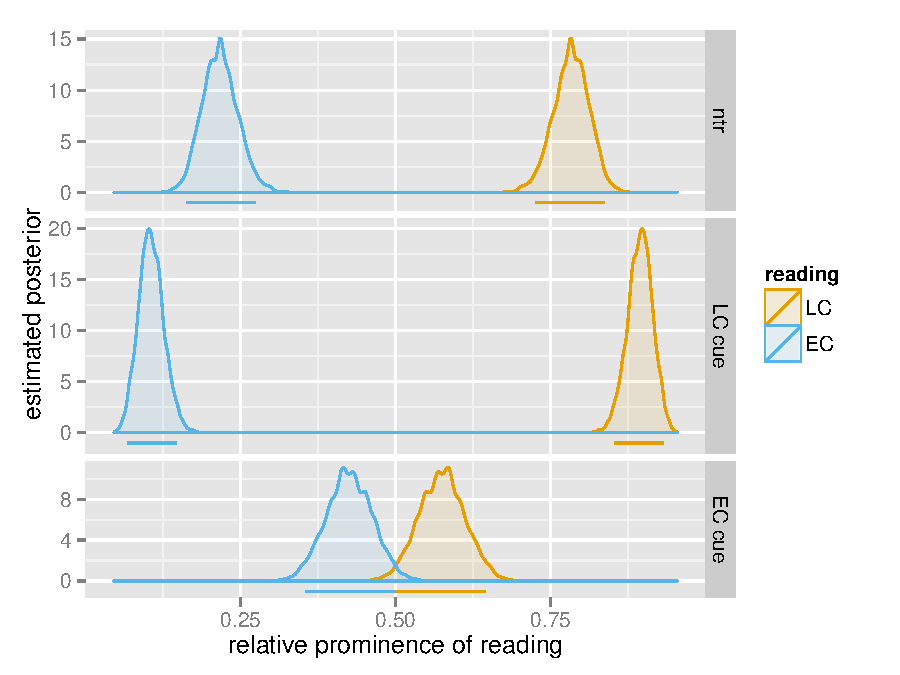
\includegraphics[width=0.8\textwidth]{pics/post_salience_TF.pdf}
  \caption{Estimated posteriors for the salience of \lc- and
    \ec-readings for different intonational cues. Lines under curves
    mark are 95\% HDIs (see Footnote~\ref{fn:HDI}).}
  \label{fig:Posterior_TF}
\end{figure}
%
Estimates for the (marginalized) posteriors over relative salience
levels for target-related controls are plotted in
Figure~\ref{fig:Posterior_TF}. The results are exactly as we would
expect them to be. Given our data, we should believe that the
\lc-reading is most prominent. The level of prominence varies with
accentuation. Under prosody that we hypothesized would favor the
\lc-reading, the contrast is most pronounced. Under accentuation that
we hypothesized favors the \ec-reading we are no longer justified in
believing with certainty that the \lc-reading is preferred (by
comparison of 95\% HDIs, see below).\footnote{\label{fn:HDI} A 95\%
  Highest Density Interval (HDI) is a convex region of values over
  which 95\% of the distribution's probability density is divided,
  such that no value outside of that region has higher probability
  density than any point within
  \citep{Kruschke2011:Doing-Bayesian-}. Intuitively speaking, the 95\%
  HDI is the set of values which we may believe to be true with some
  confidence; what falls outside this region is what can be excluded
  safely.}

\begin{figure}
  \centering
  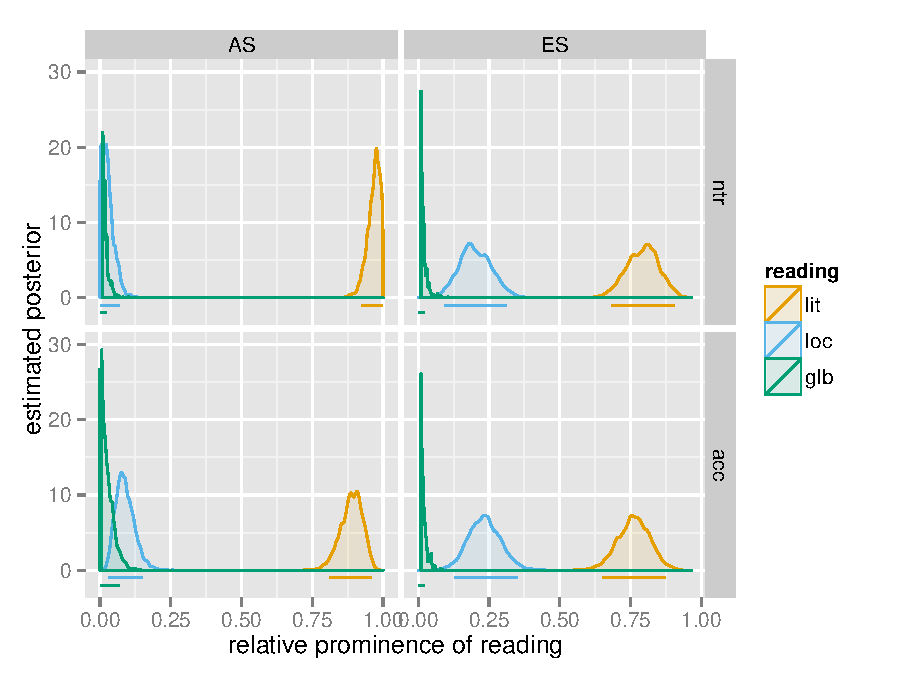
\includegraphics[width=0.8\textwidth]{pics/post_salience.pdf}
  \caption{Posteriors over relative salience of target readings in
    critical conditions.}
  \label{fig:Posterior_T}
\end{figure}

Estimates of posteriors over salience of readings in the critical
conditions are given in Figure~\ref{fig:Posterior_T}. In the
\es-conditions, literal readings are by far the most salient, followed
by local, followed by global readings. There does not appear to be a
significant effect of intonation (by visual comparison of 95\%
HDIs). For \as-sentences, the same preference order holds in tendency,
but we cannot assert with full confidence that local readings are
attested or that they are preferred over global readings (see below).
 
Posteriors over error rates are conceptually less interesting, and we
will skip them here. The posterior over the sequential bias parameter
is shown in Figure~\ref{fig:post_q}. Since the 95\% is clearly
entirely below .5, we have reason for believing, given the model and
our data, in a bias for late responses.

\begin{figure}
  \centering
  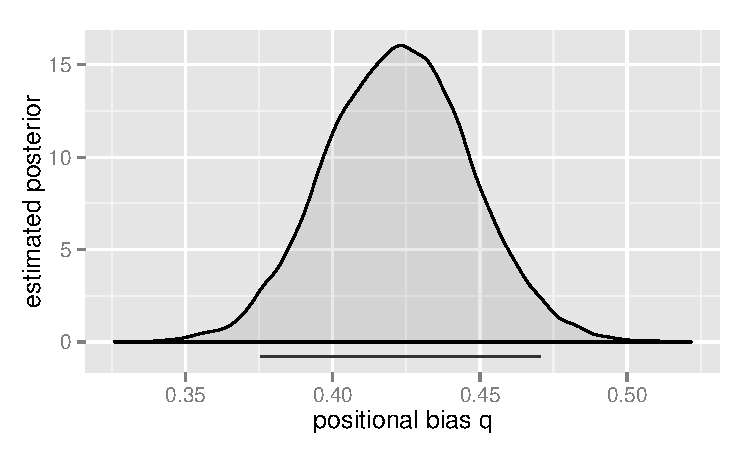
\includegraphics[width=0.5\textwidth]{pics/post_q.pdf}
  \caption{Estimated Posteriors over global sequential bias parameter
    $q$.}
  \label{fig:post_q}
\end{figure}

\paragraph{Model validation.} As a crude sanity check that our model
is able to predict the observed data, we gathered 10.000 random values
from the posterior predictive distribution and found a highly
significant correlation between these and the observed data ($R^2 =
0.987$, $p < 0.001$).

\paragraph{Hypothesis testing.} We are chiefly interested in two
questions: (i) which readings are available? and (ii) what is the
preference order over readings?

The first question can be answered by looking at the HDIs of the
posteriors of the candidate readings. We would like to check the
hypothesis that a given reading is unavailable, i.e., its activation
value in the probabilistic model is equal to 0, or close to zero for
practical purposes (Region of Practical Equivalence, ROPE). We reject
the ``null-hypothesis'' that the true value is 0 if its ROPE lies
entirely outside the 95\% HDI; we accept the ``null-hypothesis'' if
the ROPE lies entirely within the 95\% HDI
\citep[][Ch.~12]{Kruschke2011:Doing-Bayesian-}. The following table
lists approximations of the 95\% HDIs for each condition and reading:

\begin{center}
  \begin{tabular}{lllllll}
    & lit & loc & glb & \\ \midrule
    \as-ntr & $(0.924 , 1)$ & $(0 , 0.068)$
    & $(0 , 0.022)$ \\
    \as-acc 
    & $(0.816 , 0.964)$
    & $(0.028 , 0.152)$
    & $(0 , 0.066)$ \\
    \es-ntr 
    & $(0.665 , 0.873)$
    & $(0.117 , 0.323)$
    & $(0 , 0.024)$ \\
    \es-acc 
    & $(0.634 , 0.851)$
    & $(0.139 , 0.356)$
    & $(0 , 0.022)$ 
  \end{tabular}
\end{center}

\noindent We should thus accept the hypothesis that there are no
global readings at all, and no local readings for \as-sentence under
neutral intonation. There is support for a belief in local readings in
the \as-acc condition up to a ROPE of $[0;0.028)$.

The preference relations between readings can be checked in a similar
way. We look at the posterior beliefs about the \emph{differences} of
activation strengths and ask whether these posterior beliefs allow us
to safely conclude that differences are bigger than zero or not. It is
obvious enough that literal readings are always the most preferred,
and that local readings are preferred over global readings for
\es-sentences. Figure~\ref{fig:PostDiffTAS} shows the posteriors over
differences for the only non-trivial cases, namely those between local
and global readings for \as-sentences. Since the 95\% HDIs include 0,
the data provides no ground for confidence that, given the model,
local readings of \as-sentences are preferred over global ones,
despite the obvious tendency. In sum, with the exception of remaining
uncertainty about local readings of \as-sentences, the model and the
data suggest that global readings are absent entirely, while literal
readings are preferred over local readings.

\begin{figure}
  \centering
  \subfloat[neutral][]{
      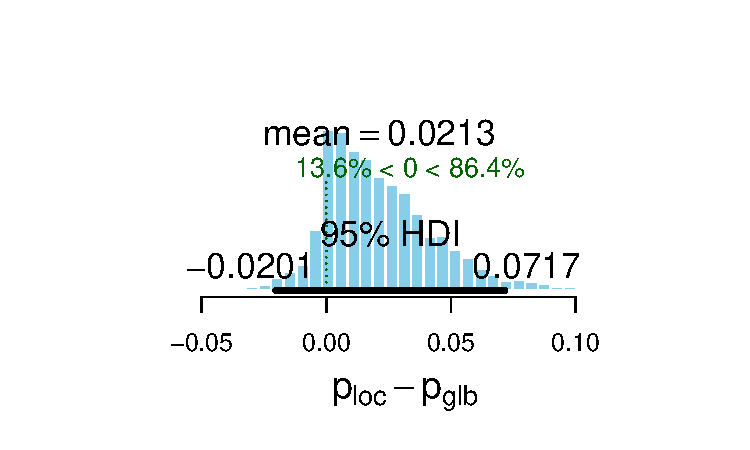
\includegraphics[width=0.45\textwidth]{PostDiffT_ASntr.pdf}
  }
  \hfill
  \subfloat[accented][]{
      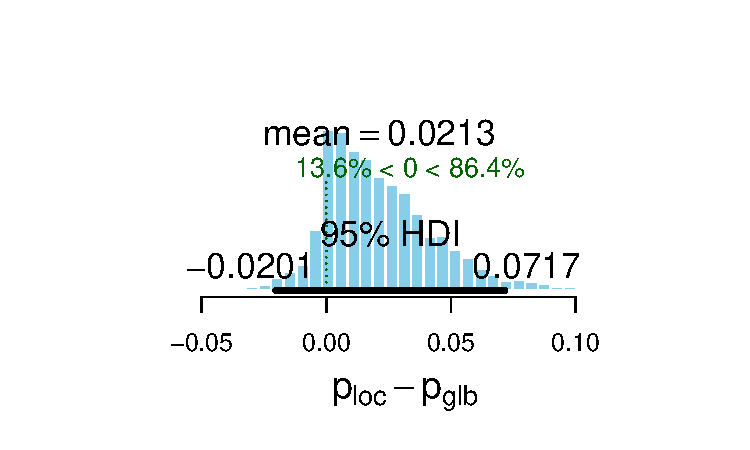
\includegraphics[width=0.45\textwidth]{PostDiffT_ASntr.pdf}
  }
  \caption{Posteriors over differences between salience levels for
    local and global readings of \as-sentences.}
  \label{fig:PostDiffTAS}
\end{figure}

\subsection{Discussion}
\label{sec:discussion-1}

\paragraph{Summary \& Interpretation.} High scores of success clearly
indicate that participants understood the incremental verification
task and were in general able to give judgements at the earliest
possible point in a picture sequence.  Moreover, results obtained for
the preference-related controls show that our design is able to detect
multiple readings and preferences among these. Crucially, the amount
of response types for \lc- and \ec-readings reflected the known
preference for the former, \emph{irrespective} of the order in which
each reading could first be judged in a given sequence.  Finally, the
incremental verification task was generally sensitive to
prosody. However, prosodic effects were restricted to the
preference-related controls. As expected, in these conditions, the
dispreferred \ec-reading was chosen significantly more often when
supported by prosodic phrasing. Interestingly, contrastively accenting
scalar \emph{some} had no effect on the observed decisions in the
target conditions. Crucially, local readings occurred in both \as- and
\es-sentences, independently of prosody. Finally, closer examination
of the participants' decisions revealed two groups: participants in
the first group consistently gave answers corresponding to local
readings, whereas participants in the second group consistently showed
a literal interpretation.

Given the overall pattern of results, the most straightforward 
explanation of the observed data is the hypothesis that the actual 
preferences among readings for both \as- and \es-sentences alike are:

\begin{exe}
  \ex \label{bsp:observed-preferences} \lit \ > \ \loc \ \ ( > \glb)
\end{exe}

\noindent where it is unclear whether the global readings are entirely
unavailable or simply severely dispreferred. Crucially, our data
attests local readings independently of prosody, albeit that local
readings are not preferred to literal readings and given, as it seems,
only by a small, but substantial number of consistent localists.

These findings are hard to for traditionalism and grammaticalism
alike, as no version of either would predict the pattern in
(\ref{bsp:observed-preferences}).  Traditionalism, if left on its own,
fails to predict local readings, while grammaticalism, when it relies
on the strongest meaning hypothesis, fails to predict the right
preference order and, more importantly, cannot explain the absence of
answers indicative of a global reading. Let's look more closely at
each position in turn.

For traditionalism, the absence of global readings \textit{per se} can
be explained, for instance, by proposing that the extra assumptions
needed to derive global readings are not standardly available (as in
the weak variety of traditionalism).  Alternatively, traditionalists
could argue that the task's rather high processing demands lead to a
suppression of global readings, in line with the findings of
\citet{NeysDe-NeysSchaeken2007:When-People-Are} that working memory
load negatively affects the number of scalar implicature responses in
sentence verification tasks. However, it then remains unclear why
memory effects should be restricted to global readings.  As a result,
approaches like the unrestricted variety of traditionalism thereby
loose the possibility of accounting for local readings of
\as-sentences.\fn{Remember that unrestricted traditionalism, as we
  called it, can account for local readings of \as-sentences by
  assuming that a sentence of the form \emph{Some of the $X$ are
    related to some of the $Y$} is a feasible alternative.} This is
because unrestricted traditionalism explains local and global readings
of \as-sentences in essentially the same manner. On top of that,
traditionalism cannot explain local readings for
\es-sentences. Resorting to the intonational markedness hypothesis
does not help improve predictions of traditionalism. The latter would
predict an increase in local readings in the accented conditions, and
presumably an absence of local readings in the unaccented
conditions. Neither was observed. Local readings were observed in the
accented as well as in the unaccented condition, thus countering
previous traditionalist suggestions that local readings are to be
attributed to specific pragmatic mechanisms. Other mechanisms might be
hypothesized as the source of local readings (and we will look at some
obvious candidates below), but that does not as such save
traditionalism. Traditionalism, even if supplemented with the
intonational markedness hypothesis, cannot explain
(\ref{bsp:observed-preferences}), but needs an additional explanation
of local readings for \emph{both} \as- \emph{and} \es-sentences.

Grammaticalism, on the other hand, fails to predict the preference
relation in (\ref{bsp:observed-preferences}), in particular the
absence of answers indicative of global readings. This is because
(\ref{bsp:observed-preferences}) strictly contradicts the strongest
meaning hypothesis in either of the two varieties suggested by
\citet{ChierchiaFox2008:The-Grammatical}. This shows most clearly in
the fact that both versions of the strongest meaning hypothesis
predict that local readings of \as-sentences are preferred over
literal ones. The problem, therefore, seems to be the selection of
readings by the strongest meaning hypothesis. In fact, if
(\ref{bsp:observed-preferences}) is the actual preference over
readings, then the strongest meaning hypothesis is also conceptually
on the wrong track, because no account that merely looks at the
logical strengths of readings can plausibly predict the preference
pattern in (\ref{bsp:observed-preferences}) for both \as- and
\es-sentences at the same time. 

Summing up so far, the existing versions of traditionalism, even if
aided by the intonational markedness hypothesis, and grammaticalism
cannot explain the present results. What would it take to amend either
framework to make it fit the data we observed? Traditionalism would
need to explain the possibility of local readings of intonationally
unmarked sentences. To do so within a traditionalist framework seems
impossible, so the most common approach is to explain putative
evidence for local readings away as the result of some other
phenomenon, such as typicality or contrast
\citep{Tielvan-Tiel2012:Embedded-Scalar,GeurtsTielvan-Tiel2013:Scalar-expressi}. We
argue below that neither explanation plausibly applies in the
incremental verification task. On the other hand, what grammaticalism
would have to change is the selection criterion over preferred
readings, i.e., to reconsider the strongest meaning
hypothesis. Turning away from comparisons of logical strength, a
\emph{prima facie} plausible selection criterion that produces
(\ref{bsp:observed-preferences}) is ready at hand: if we assume that
each insertion of the $\exh(\cdot)$ operator is \emph{costly}
anti-proportional to the depth of its embedding under other logical
operators, then we derive a preference of literal readings over local
ones over global ones. Whether such an \emph{economy principle} is
sound and in line with further empirical data would then be an
interesting matter of further investigation.

It is worth noting that an alternative theory of scalar implicature
explains the observed preference ordering
(\ref{bsp:observed-preferences}) in a completely straightforward
manner.  \emph{Conventionalism} (also sometimes called
\emph{lexicalism}) proposes that if the upper-bound inference from
\emph{some} to \emph{some but not all} occurs frequently, it would be
inefficient to execute over and over again the Gricean reasoning that
traditionalists propose
\citep[e.g.][]{LevinsonPresumptiveMeanings2000,Chierchia:2004_ScalarImplicatures}. Conventionalism
therefore assumes that scalar inferences have become routinized,
hard-wired, so much so that there are two lexical entries for a scalar
item like \emph{some}, one with logical meaning \emph{some and maybe
  all} and one with the upper-bounded meaning \emph{some but not
  all}. \citet{LevinsonPresumptiveMeanings2000} proposed that the
latter is the preferred default meaning, a position which has
therefore ofttimes be addressed as \mymark{defaultism}. Unfortunately,
defaultism has strong empirical evidence against it, because several
processing studies show that the computation of scalar inferences
appears to be time- and effort-consuming, when they do arise, not when
they do not
\citep[see][]{BrehenyKatsos2006:Are-Generalised,BrehenyKatsos2008:Experimental-In,NeysDe-NeysSchaeken2007:When-People-Are}. But
there is also competing evidence that scalar inferences are available
in immediate, low-level processes, such as the resolution of
referential expressions in a visual-world paradigm
\citep{GrodnerKlein2010:Some-and-Possib}. For our purposes, it is
interesting to note that the preference relation in
(\ref{bsp:observed-preferences}) is predicted by the dual of
defaultism, which has not been defended in the literature as far as we
know, which posits a lexical ambiguity but predicts that the logical
meanings are \emph{ceteris paribus} preferred over the upper-bounded
meanings.

Unfortunately, there are problems with conventionalism, no matter
which lexical reading is assumed to be preferred, that seem to require
that it be backed up by traditionalism
\citep[e.g.][]{Sauerland2012:The-Computation}.\fn{\citet{Sauerland2012:The-Computation}
  eventually dismisses even conventionalism backed up by
  traditionalism in favor of grammaticalism based on cases of
  so-called \emph{intermediate implicatures}, where what seems to be
  necessary is the insertion of an exhaustivity operator in
  intermediate scope position \citep[see][for
  details]{Sauerland2012:The-Computation}. Appreciation of such
  intermediate implicatures requires more argumentation, involving a
  discussion of \emph{Hurford's constraint}
  \citep[see][]{FoxSpector:Economy-and-Emb,ChierchiaFox2009:Hurfords-Constr,ChierchiaFox2008:The-Grammatical},
so we skip this here.}
For instance, conventionalism cannot account for \emph{indirect
  implicatures}, such as the inference from
(\ref{bsp:indirect-SI-Target}) to (\ref{bsp:indirect-SI-Inference})
which cannot be explained by positing a lexical ambiguity for
\emph{all}.

\begin{exe}
  \ex \label{bsp:indirect-SI}
    \begin{xlist}
      \ex \label{bsp:indirect-SI-Target} Hans did not solve all of the problems.
      \ex \label{bsp:indirect-SI-Inference} Hans solved some of the problems.
    \end{xlist}
\end{exe}

\noindent In the context of the present study, this would then be good
news for traditionalism, because a combined
traditionalism+conventionalism would predict the observed data
well. The combined position would even be able to explain something
that grammaticalism cannot make sense of as easily, namely the
observation that there were rather consistent localists among the
participants of our study. The combined tradionalism+conventionalism
could explain this by the assumption that some (lazy?, smart?)
speakers have made a conventionalized upper-bound meaning entry for
scalar \emph{some} while others keep computing things on the fly. It
is not clear how grammaticalism can account for the intra-subjective
consistency. Still, this is not an argument \emph{for} traditionalism,
because the point remains that traditionalism as such fails to predict
the observed data.
  

In sum, if the interpretation of our data as suggested here is
correct, then both traditionalism and grammaticalism are in need of
revision. Traditionalism must explain the availability of local
readings, grammaticalism must revise its selection criterion among
readings.

\paragraph{Some Potential Objections.} There are a number of
conceivable objections to our interpretation of the presented
results. We will consider the most pressing ones in the following.

To begin with, it could be questioned whether our design reliably
indicates the preference relation in (\ref{bsp:observed-preferences})
among readings of our target sentences. After all, our incremental
verification task might simply select for the weakest possible
reading. This idea can be grounded in the observation that the
preferred \lc-readings of our target-related controls entail the
dispreferred \ec-readings. It could thus be argued that the difference
in responses for preference-related controls are due to the entailment
properties, not the known preference relation over \lc- and
\ec-readings. However, this does not explain why the distribution of
responses in the target conditions are obviously not governed by
logical strength. In fact, it is a very noteworthy point that although
entailment relations among readings differ between \as- and
\es-sentences, the observed response pattern does not. (This is what
is at the heart of the problem for a grammaticalism that relies on the
strongest meaning hypothesis.)

A related objection would be that maybe it is not feasible to actually
compare results from the preference-related controls to results from
our target conditions, because the source of different readings is
fundamentally different. In the former we have a syntactic ambiguity,
in the latter a small number of competing putative pragmatic
enrichments. The former is a case of perceived ambiguity (some of our
subjects reported this), the latter arguably is not
\citep[see][]{GeurtsPouscoulous2009:Embedded-Implic}. So perhaps even
if the distribution of responses is indicative of the known preference
patterns in preference-related controls, this would not necessarily
mean that the distribution of responses in target conditions is
indicative of preference relations.

Although we cannot rule out that the incremental verification task
detects preferences among multiple readings only for some sources of
variability in readings and not others, it is by no means clear why
this should be so. The burden of argument is on the sceptic. But even
if we assume that the incremental verification task is incapable of
reliably indicating preferences among candidate pragmatic enrichments
of the relevant kind, then it should at least be able to indicate
availability of readings. So if we deny the observed response patterns
the power to indicate preference, what should the information about
availability of readings be that we may safely infer from it? It
should be that local readings are available and that global readings
are not. But that is not predicted by either traditionalism or
grammaticalism. The former cannot explain the substantial number of
local responses, the latter doesn't explain the absence of global
responses.

A third objection could be that pictures in our tasks may unduly
overemphasize the contrast between cases where items are connected
with all or merely some but not all of their surrounding shapes. This
is essentially the line of argument pursued by
\citet{GeurtsTielvan-Tiel2013:Scalar-expressi} against the data
reported by \citet{ChemlaSpector2010:Experimental-Ev} in support of
local readings of
\es-sentences. \citeauthor{GeurtsTielvan-Tiel2013:Scalar-expressi}
show that the strength of agreement to an \es-sentence on a 7-point
Likert-scale depends on a visual contrast between, on the one hand,
one element connected to some but not all of its surrounding shapes,
and, on the other hand, a variable number of elements connected to all
of their surrounding shapes. When two universally connected elements
are present, the mean rate of agreement with a suitable \es-sentence
is higher than when only one is present. So, maybe our displays
similarly provoked local readings because of an overemphasized visual
contrast.

This cannot be a plausible explanation for the number of local
responses we found in our study. Although it is true that the critical
position for judging the local reading is a picture with a high visual
contrast in the above sense (see Figure~\ref{fig:exseqES}), a purely
contrast-based explanation of the local responses in our data is not
feasible for two reasons. The first is that visual contrast does not
explain how subjects ever even got past the second critical position
where the sentence can be judged false under its literal reading. At
this position there is a visual contrast of the alleged kind but it is
as small as possible. So something must have motivated subjects
already at this position to continue unraveling, given that they were
generally able of exiting at the earliest possible location, as
evidenced by ceiling success rates in our positional controls. A second
argument that casts doubt on a contrast-based explanation is that our
study elicited categorical truth-value judgements. Unlike in
\citeauthor{ChemlaSpector2010:Experimental-Ev}'s
(\citeyear{ChemlaSpector2010:Experimental-Ev}) and
\citeauthor{GeurtsTielvan-Tiel2013:Scalar-expressi}'s
(\citeyear{GeurtsTielvan-Tiel2013:Scalar-expressi}) experiments, we
did not record degrees of agreement with a statement. But it is hardly
plausible that the visual contrast in a picture like in
Figure~\ref{fig:subfig1} alone is enough to overrule a truth-value
judgment so as to contradict the semantic meaning (even when there is
no intonational markedness to support such a
reinterpretation). Ultimately, however, even if the local answers in
our study are contrast effects, the verdict remains that
traditionalism can not account for that piece of the data unless aided
by yet another auxiliary and grammaticalism cannot explain why it is
relatively dispreferred.

% A fourth major conceivable objection maintains that we cannot rule out
% that the way we realized the intonational markedness in the accented
% conditions was not the right kind of intonational
% markedness. Therefore the intonational markedness hypothesis that
% links an increase in local readings to intonation might not be
% falsified by our results. Although true, this still does not help
% vindicate traditionalism, for even without marked intonation local
% readings were available.

Also, we should address the obvious worry that maybe our results
could have been the product of typicality after all. Remember that
\citet{Tielvan-Tiel2012:Embedded-Scalar} and
\citet{GeurtsTielvan-Tiel2013:Scalar-expressi} argue that the
distribution of responses to \as-sentences found by
\citet{CliftonDube2010:Embedded-Implic}, as well as
\citet{ChemlaSpector2010:Experimental-Ev} could be explained by
differences in how typical representations for an \as-sentence the
presented pictures were. To apply typicality-explanations to the
incremental verification task, one would have to reason about the
typicality of parts of pictures or to figure in subjects' expectations
of pictorial typicality given their uncertainty about parts of the
picture that they have not yet seen. On intuitive grounds, we take
either extension to be far-fetched and implausible. But even if this
line of explanation can be plausibly extended to incrementally
revealed picture verification, this does not as such save the day for
traditionalism or grammaticalism, because, as argued above, typicality
effects are arguably insufficient to explain the change in categorical
truth-value judgement that we found in our experiment.

% Still, graphical properties might affect judgments in the worst
% case. In the first step of the \as-condition local and global readings
% cannot be judged, yet. Therefore, graphical properties should not
% affect judgments if participants have one of these readings in
% mind. If participants have a literal reading in mind, the worst case
% scenario is that they refrain from judging the sentence as true at
% this point due to some, say, atypical, graphical property of the
% picture. The situation is similar at the second step. The local
% reading is still not decidable. Therefore, graphical properties should
% not play a role if participants have a local reading in mind. A
% positive judgment might, however, be a delayed judgment of a literal
% reading. Again, the worst case scenario for our purpose is that
% participants refrain from answering because of graphical
% properties. At the last step the local reading requires a negative
% judgment. Now, we could obtain delayed negative responses from literal
% or global readings because the graph as a whole is, e.g., logically
% true but atypical with respect to these readings. These kinds of
% judgments would be indistinguishable from local responses. Note,
% however, that we have no reason to believe that typicality has large
% effects, because, given the results from van Tiel, the picture as a
% whole is expected to be one of the more typical situations for
% \as-sentences. Still, we cannot exclude the possibility that graphical
% properties of the pictures might have the described effect. In the
% \es-conditions this type of effect is, however, entirely impossible
% since the literal and global reading is plainly false given the
% initial parts as well as the whole graph. Summing up, in the worst
% case, which we consider implausible, graphical effects might lead to
% an enhanced number of local responses in the \as- as compared to the
% \es-condition. We have to keep this possibility in mind. We want to
% stress, however, that the design presented here improves on previous
% studies with respect to possible graphical effects.

\paragraph{Future Directions.} The data obtained from our experiment
also raises a number of issues for future research. Firstly, we found
a tendency of subjects to give literal or local answers rather
consistently. This seems to be related to what has been reported in a
number of previous studies on unembedded \emph{some}, where a tendency
was found as well in subjects to either consistently interpret
\emph{some} `semantically' as \emph{some and possibly all} or to
consistently interpret it `pragmatically' as \emph{some and not all}
\citep[e.g.][]{NoveckPosada2003:Characterizing-,BottNoveck2004:Some-Utterances,DegenTanenhaus2012:Processing-Scal}. This
inter-subjective consistency has not been paid any attention to in
previous studies on embedded scalar items. It would be interesting to
test whether there is any indication of a correlation between, on the
one hand, subjects' tendencies to give literal vs.~local answers for
embedded occurrences of \emph{some} and, on the other hand, subjects'
tendencies to interpret unembedded \emph{some} semantically or
pragmatically. If such a correlation exists, it would point towards
the possibility that different subjects may even have different
lexical representations of \emph{some} or possibly employ different
processes of interpreting it. If so, this would severely mix up the
theoretical landscape and should also be taken into account in any
further study on the processing of scalar items.

Secondly, given the scarce literature on the topic, more research into
the role of intonational markedness on pragmatic interpretation is
clearly needed. Claims about the correlation of certain
interpretations with certain patterns of intonation are frequently
made in the theoretical literature, but often only backed up by
introspection and not made precise in their commitment to the exact
kind of intonational pattern that is hypothesized to be relevant. The
intonational markedness hypothesis, for instance, seems \emph{prima
  facie} plausible, but we did not find any evidence for it in our
experiment. This much is not yet any direct evidence against it
either, because it is certainly possible that the contrastive accents
we realized in our experiments, although the most plausible and in
line with current theorizing about German contrast marking, was not
the right kind of intonational markedness. This shows for one that
claims about the putative effects of intonation and prosody must be
more carefully phrased and filled with detail, but also points to
further empirical research. The combination of production experiments
the output of which is fed into a subsequent interpretation experiment
comes to mind as a first natural continuation.


\section{Conclusions}
\label{sec:conclusions}

We tested experimentally the predictions of traditionalism and
grammaticalism with respect to the availability of and preferences
over three types of conceivable pragmatic readings of two types of
sentences, in which scalar \emph{some} occurred in the scope of either
a monotonic quantifier \emph{all} or the non-monotonic quantifier
\emph{exactly one}. To avoid potential confounds of the pictorial
material, such as through typicality or contrast
\citep{Tielvan-Tiel2012:Embedded-Scalar,GeurtsTielvan-Tiel2013:Scalar-expressi},
we employed an incremental verification task \citep{Conroy2008}, in
which subjects were presented with partially covered pictures and
asked to uncover the picture sequentially until they felt able to give
a categorical truth-value judgements. Sentence material was presented
auditorily and contrastive stress on embedded \emph{some} was
manipulated so as to test the intonational markedness hypothesis,
which is often used to supplement traditionalism. Both traditionalism
and grammaticalism do not predict our data well.  Traditionalism fails
to account for the non-negligible number of responses indicating local
readings even for intonationally unmarked sentences. Grammaticalism
fails to predict the absence of answers indicative of global readings
and the relative abundance of answers indicative of literal readings.



\newpage

\appendix

\section{The auditory sentence material}
\label{sec:audit-sent-mater}


\begin{table}[!hp]
  \centering
  
  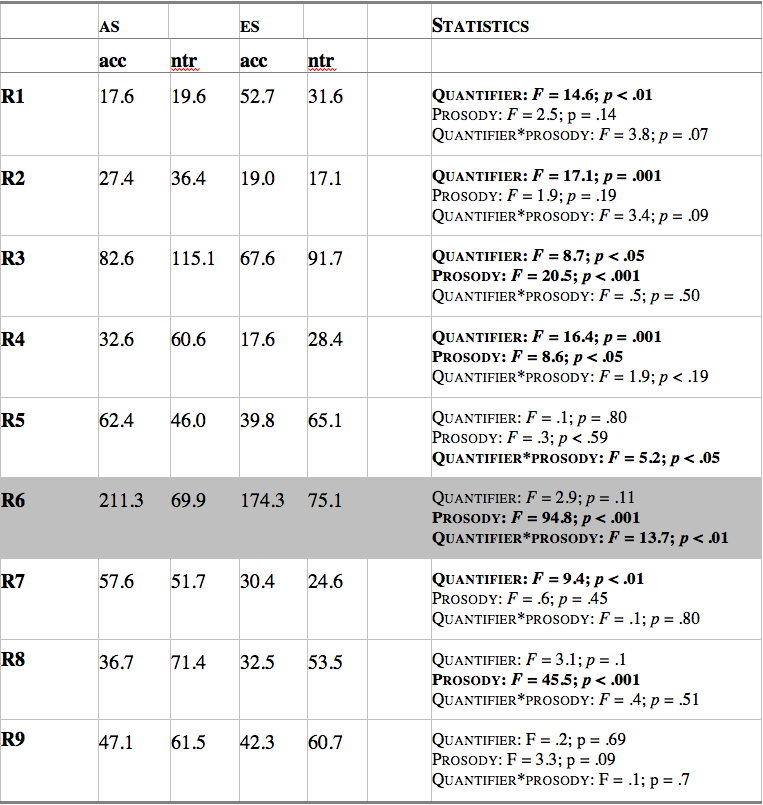
\includegraphics[width=\textwidth]{../pictures/Acoustics/Table-B.png}

  \caption{Difference between minimal and maximal F0 values in Hz for
    each of the single words in the target sentences. Region 6
    corresponds to the determiner \emph{einigen}.} 
  \label{tab:table-B}
\end{table}


\begin{table}[!hp]
  \centering
  
  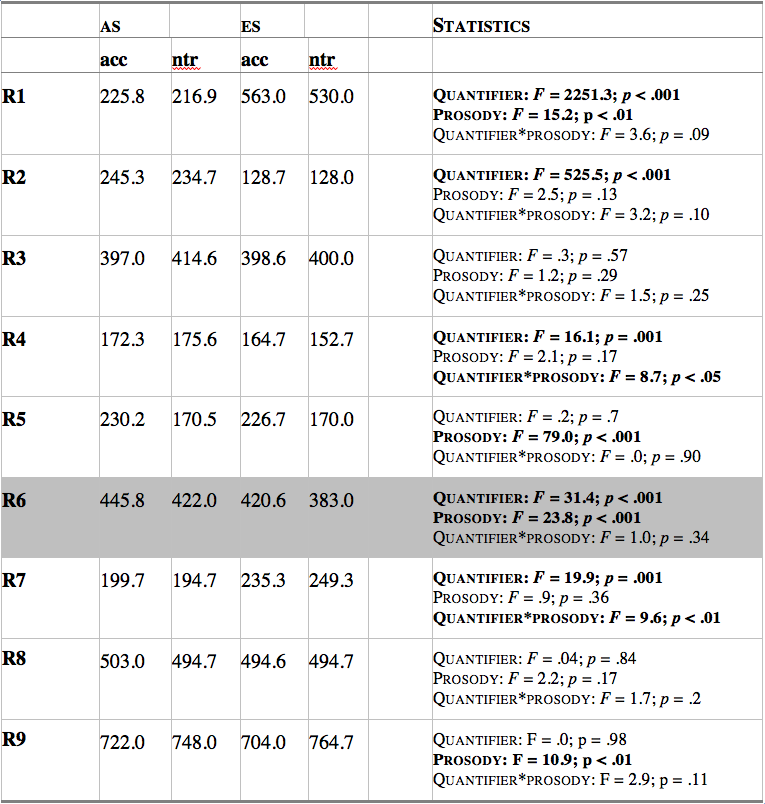
\includegraphics[width=\textwidth]{../pictures/Acoustics/Table-A.png}

  \caption{Durational values in ms for each of the single regions in the target sentences. 
  Region 6 corresponds to the determiner \emph{einigen}.}
  \label{tab:table-A}
\end{table}


\begin{table}[hp]
  \centering
  
  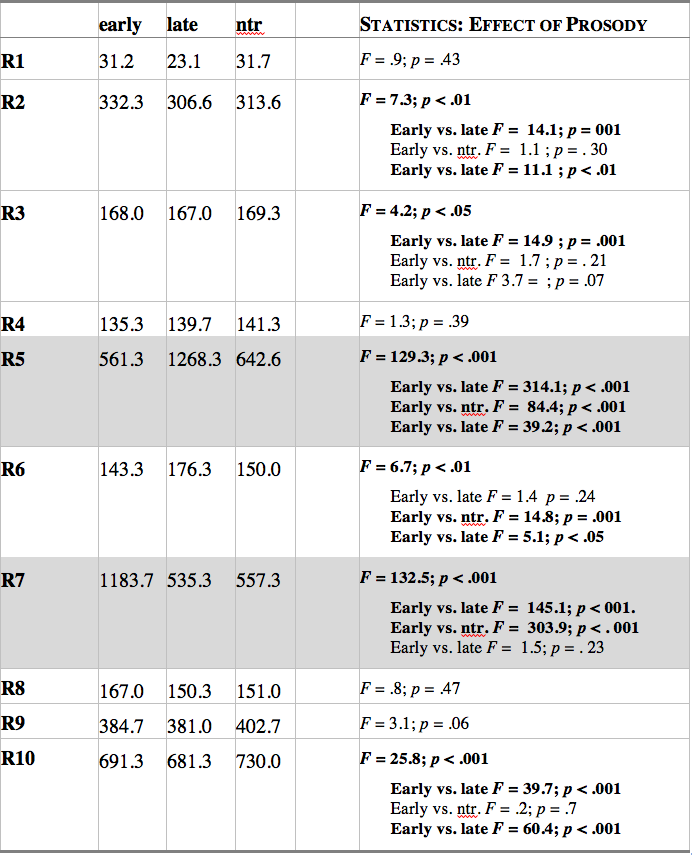
\includegraphics[width=\textwidth]{../pictures/Acoustics/Table-D.png}

  \caption{Difference between minimal and maximal F0 values in Hz  
  for each of the single regions in
    the preference-related fillers. Regions 5 and 7 correspond to the
    nouns preceding the boundaries.}  
  \label{tab:table-D}
\end{table}


\begin{table}[hp]
  \centering
  
  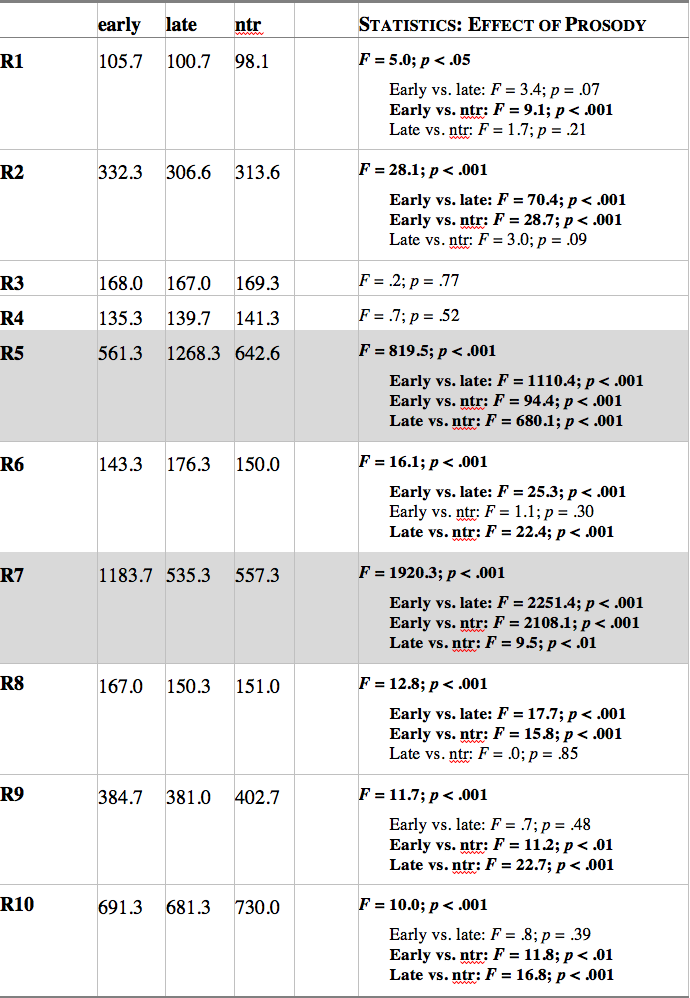
\includegraphics[width=\textwidth]{../pictures/Acoustics/Table-C.png}

  \caption{Durational values in ms for each of the single regions in
    the preference-related fillers. Regions 5 and 7 correspond to the
    nouns preceding the boundaries.}  
  \label{tab:table-C}
\end{table}


%\paragraph{Targets.} Table~\ref{tab:table-A} shows the durational values for each of
%the single regions in the sentence. Crucially, durational values of
%accented determiners were significantly increased as opposed to their
%non-accented counterparts. Overall, \acro{Quantifier} effects were
%observed, which might be attributed to the above-mentioned lexical
%differences, as well as to the fact that \es-structures generally
%contained fewer words, thus leading to a tendency of a durational
%decrease for each of the single words.
%
%Differences between maximal and minimal F0 values for each of the
%single words in the sentence are depicted in
%Table~\ref{tab:table-B}. As is descriptively evident, accented
%determiners showed a larger F0 range compared to unaccented versions,
%an effect which is confirmed by statistical analyses. An additional
%\acro{Quantifier}*\acro{Prosody} interaction indicates that these
%differences are even more pronounced in the \as-condition. Finally,
%comparable to the durational analyses, \acro{Quantifier} effects were
%observed when conditions exhibited lexical differences.
%
%Finally, differences between maximal and minimal F0 values for each of
%the single words in the sentence are given in
%Table~\ref{tab:table-D}. Again, the most reliable differences occur at
%the boundary regions.

%\paragraph{Preference-related fillers.} Table~\ref{tab:table-C} shows the
%durational values of each of the single words in the sentence. As is
%descriptively evident, the largest durational differences were
%realized at the boundary regions (i.e. Region 5 and Region
%7). Interestingly, small differences between conditions also yielded
%significance at other positions, suggesting that our speaker produced
%the different conditions very consistently (i.e., with little
%variance).

\newpage

\printbibliography[heading=bibintoc]

\end{document}
